\documentclass[onecolumn,,10pt]{IEEEtran}
\let\labelindent\relax
%\documentclass[3p,10pt]{elsarticle}
%\let\labelindent\relax
\usepackage{enumitem}
\usepackage{etex}
\usepackage{amssymb,amsfonts,amsmath,amsthm}
\usepackage{graphicx}
\usepackage[usenames,x11names, dvipsnames, svgnames]{xcolor}
\usepackage{amsmath,amssymb}
\usepackage{dsfont}
\usepackage{amsfonts}
\usepackage{mathrsfs}
\usepackage{texshade}
\usepackage{hyperref}
\hypersetup{
  colorlinks=true,
  linkcolor=black,
  citecolor=black,
  filecolor=black,
  urlcolor=DodgerBlue4,
  breaklinks=false,
  % linkbordercolor=red,% hyperlink borders will be red
  % pdfborderstyle={/S/U/W 1}% border style will be underline of width 1pt
}
\usepackage{array}
\usepackage{xr}
\usepackage{verbatim}
% \usepackage{multirow}    
% \usepackage[T1,euler-digits]{eulervm}
% \usepackage{times}
% \usepackage{pxfonts}
\usepackage{tikz}
\usepackage{pgfplots}
\usetikzlibrary{shapes,calc,shadows,fadings,arrows,decorations.pathreplacing,automata,positioning}
\usetikzlibrary{external}
\usetikzlibrary{decorations.text}
\usepgfplotslibrary{colorbrewer} 

\tikzexternalize[prefix=./Figures/External/]% activate externalization!
\tikzexternaldisable
% \addtolength{\voffset}{.1in}  
\usepackage{geometry}
\geometry{a4paper, left=.65in,right=.65in,top=.8in,bottom=0.7in}

\addtolength{\textwidth}{-.1in}    
\addtolength{\hoffset}{.05in}    
\addtolength{\textheight}{.1in}    
\addtolength{\footskip}{0in}    
\usepackage{rotating}
\definecolor{nodecol}{RGB}{240,240,220}
\definecolor{nodeedge}{RGB}{240,240,225}
\definecolor{edgecol}{RGB}{130,130,130}
\tikzset{%
  fshadow/.style={      preaction={
      fill=black,opacity=.3,
      path fading=circle with fuzzy edge 20 percent,
      transform canvas={xshift=1mm,yshift=-1mm}
    }} 
}
\usetikzlibrary{pgfplots.dateplot}
\usetikzlibrary{patterns}
\usetikzlibrary{decorations.markings}
\usepackage{fancyhdr}
\usepackage{mathtools}
\usepackage{datetime}
\usepackage{comment}
%% ## Equation Space Control---------------------------
\def\EQSP{3pt}
\newcommand{\mltlne}[2][\EQSP]{\begingroup\setlength\abovedisplayskip{#1}\setlength\belowdisplayskip{#1}\begin{equation}\begin{multlined} #2 \end{multlined}\end{equation}\endgroup\noindent}
\newcommand{\cgather}[2][\EQSP]{\begingroup\setlength\abovedisplayskip{#1}\setlength\belowdisplayskip{#1}\begin{gather} #2 \end{gather}\endgroup\noindent}
\newcommand{\cgathers}[2][\EQSP]{\begingroup\setlength\abovedisplayskip{#1}\setlength\belowdisplayskip{#1}\begin{gather*} #2 \end{gather*}\endgroup\noindent}
\newcommand{\calign}[2][\EQSP]{\begingroup\setlength\abovedisplayskip{#1}\setlength\belowdisplayskip{#1}\begin{align} #2 \end{align}\endgroup\noindent}
\newcommand{\caligns}[2][\EQSP]{\begingroup\setlength\abovedisplayskip{#1}\setlength\belowdisplayskip{#1}\begin{align*} #2 \end{align*}\endgroup\noindent}
\newcommand{\mnp}[2]{\begin{minipage}{#1}#2\end{minipage}} 
%% COLOR DEFS------------------------------------------
\newtheorem{thm}{Theorem}
\newtheorem{cor}{Corollary}
\newtheorem{lem}{Lemma}
\newtheorem{prop}{Proposition}
\newtheorem{defn}{Definition}
\newtheorem{exmpl}{Example}
\newtheorem{rem}{Remark}
\newtheorem{notn}{Notation}
%% ------------PROOF INCLUSION -----------------
\def\NOPROOF{Proof omitted.}
\newif\ifproof
\prooffalse % or \draftfalse
\newcommand{\Proof}[1]{
  \ifproof
  \begin{IEEEproof}
    #1\end{IEEEproof}
  \else
  \NOPROOF
  \fi
}
%% ------------ -----------------
\newcommand{\DETAILS}[1]{#1}
%% ------------ -----------------
% color commands------------------------
\newcommand{\etal}{\textit{et} \mspace{3mu} \textit{al.}}
% \renewcommand{\algorithmiccomment}[1]{$/** $ #1 $ **/$}
\newcommand{\vect}[1]{\textbf{\textit{#1}}}
\newcommand{\figfont}{\fontsize{8}{8}\selectfont\strut}
\newcommand{\hlt}{ \bf \sffamily \itshape\color[rgb]{.1,.2,.45}}
\newcommand{\pitilde}{\widetilde{\pi}}
\newcommand{\Pitilde}{\widetilde{\Pi}}
\newcommand{\bvec}{\vartheta}
\newcommand{\algo}{\textrm{\bf\texttt{GenESeSS}}\xspace}
\newcommand{\xalgo}{\textrm{\bf\texttt{xGenESeSS}}\xspace}
\newcommand{\FNTST}{\bf }
\newcommand{\FNTED}{\color{darkgray} \scriptsize $\phantom{.}$}
\renewcommand{\baselinestretch}{.95}
\newcommand{\sync}{\otimes}
\newcommand{\psync}{\hspace{3pt}\overrightarrow{\hspace{-3pt}\sync}}
% \newcommand{\psync}{\raisebox{-4pt}{\begin{tikzpicture}\node[anchor=south] (A) {$\sync$};
%   \draw [->,>=stealth] ([yshift=-2pt, xshift=2pt]A.north west) -- ([yshift=-2pt]A.north east); %\end{tikzpicture}}}
\newcommand{\base}[1]{\llbracket #1 \rrbracket}
\newcommand{\nst}{\textrm{\sffamily\textsc{Numstates}}}
\newcommand{\HA}{\boldsymbol{\mathds{H}}}
\newcommand{\eqp}{ \vartheta }
\newcommand{\entropy}[1]{\boldsymbol{h}\left ( #1 \right )}
\newcommand{\norm}[1]{\left\lVert #1 \right\rVert}%
\newcommand{\abs}[1]{\left\lvert #1 \right\rvert}%
\newcommand{\absB}[1]{\big\lvert #1 \big\rvert}%
% #############################################################
% #############################################################
% PREAMBLE ####################################################
% #############################################################
% #############################################################
% \usepackage{pnastwoF}      
\DeclareMathOperator*{\argmax}{argmax}
\DeclareMathOperator*{\argmin}{arg\,min}
\DeclareMathOperator*{\expect}{\mathbf{E}}
\DeclareMathOperator*{\var}{\mathbf{Var}}

\newcommand{\ND}{ \mathcal{N}  }
\usepackage[linesnumbered,ruled,vlined,noend]{algorithm2e}
\newcommand{\captionN}[1]{\caption{\color{darkgray} \sffamily \fontsize{9}{11}\selectfont #1  }}
\newcommand{\btl}{\ \textbf{\small\sffamily bits/letter}}
\usepackage{txfonts}
% \usepackage{ccfonts}
%%% save defaults
\renewcommand{\rmdefault}{phv} % Arial
\renewcommand{\sfdefault}{phv} % Arial
\edef\keptrmdefault{\rmdefault}
\edef\keptsfdefault{\sfdefault}
\edef\keptttdefault{\ttdefault}

% \usepackage{kerkis}
\usepackage[OT1]{fontenc}
\usepackage{concmath}
% \usepackage[T1]{eulervm} 
% \usepackage[OT1]{fontenc}
%%% restore defaults
\edef\rmdefault{\keptrmdefault}
\edef\sfdefault{\keptsfdefault}
\edef\ttdefault{\keptttdefault}
\tikzexternalenable
% ##########################################################
\tikzfading[name=fade out,
inner color=transparent!0,
outer color=transparent!100]
% ###################################
\newcommand{\xtitaut}[2]{
  \noindent\mnp{\textwidth}{
    \mnp{\textwidth}{\raggedright\Huge \bf \sffamily #1}

    \vskip 1em

    {\bf \sffamily #2}
  }
  \vskip 2em
}
% ###################################
% ###################################
\tikzset{wiggle/.style={decorate, decoration={random steps, amplitude=10pt}}}
\usetikzlibrary{decorations.pathmorphing}
\pgfdeclaredecoration{Snake}{initial}
{
  \state{initial}[switch if less than=+.625\pgfdecorationsegmentlength to final,
  width=+.3125\pgfdecorationsegmentlength,
  next state=down]{
    \pgfpathmoveto{\pgfqpoint{0pt}{\pgfdecorationsegmentamplitude}}
  }
  \state{down}[switch if less than=+.8125\pgfdecorationsegmentlength to end down,
  width=+.5\pgfdecorationsegmentlength,
  next state=up]{
    \pgfpathcosine{\pgfqpoint{.25\pgfdecorationsegmentlength}{-1\pgfdecorationsegmentamplitude}}
    \pgfpathsine{\pgfqpoint{.25\pgfdecorationsegmentlength}{-1\pgfdecorationsegmentamplitude}}
  }
  \state{up}[switch if less than=+.8125\pgfdecorationsegmentlength to end up,
  width=+.5\pgfdecorationsegmentlength,
  next state=down]{
    \pgfpathcosine{\pgfqpoint{.25\pgfdecorationsegmentlength}{\pgfdecorationsegmentamplitude}}
    \pgfpathsine{\pgfqpoint{.25\pgfdecorationsegmentlength}{\pgfdecorationsegmentamplitude}}
  }
  \state{end down}[width=+.3125\pgfdecorationsegmentlength,
  next state=final]{
    \pgfpathcosine{\pgfqpoint{.15625\pgfdecorationsegmentlength}{-.5\pgfdecorationsegmentamplitude}}
    \pgfpathsine{\pgfqpoint{.15625\pgfdecorationsegmentlength}{-.5\pgfdecorationsegmentamplitude}}
  }
  \state{end up}[width=+.3125\pgfdecorationsegmentlength,
  next state=final]{
    \pgfpathcosine{\pgfqpoint{.15625\pgfdecorationsegmentlength}{.5\pgfdecorationsegmentamplitude}}
    \pgfpathsine{\pgfqpoint{.15625\pgfdecorationsegmentlength}{.5\pgfdecorationsegmentamplitude}}
  }
  \state{final}{\pgfpathlineto{\pgfpointdecoratedpathlast}}
}
% ###################################
% ###################################
\newcolumntype{L}[1]{>{\rule{0pt}{2ex}\raggedright\let\newline\\\arraybackslash\hspace{0pt}}m{#1}}
\newcolumntype{C}[1]{>{\rule{0pt}{2ex}\centering\let\newline\\\arraybackslash\hspace{0pt}}m{#1}}
\newcolumntype{R}[1]{>{\rule{0pt}{2ex}\raggedleft\let\newline\\\arraybackslash\hspace{0pt}}m{#1}}




\newcommand{\drhh}[8]{
  \begin{axis}[semithick,
    font=\bf \sffamily \fontsize{7}{7}\selectfont,
    name=H2,
    at=(#4), anchor=#5,
    xshift=.3in,
    yshift=-.3in,
    width=\WDT, 
    height=\HGT, 
    title={{\LARGE G } ROC area distribution (Out-of-sample)}, 
    title style={align=right, },legend cell align=left,
    legend style={ xshift=3.5in, yshift=-.6in, draw=white, fill= gray, fill opacity=0.2, 
      text opacity=1,},
    axis line style={black!80, opacity=0,   thick,,ultra thin, rounded corners=0pt},
    axis on top=false, 
    xlabel={ROC area},
    ylabel={probability},
    ylabel style={yshift=-.25in},
    xlabel style={yshift=.1in},
    grid style={dashed, gray!50},
    % grid,
    axis background/.style={top color=gray!1,bottom color=gray!2},
    enlargelimits=false, 
    scale only axis=true,
    ymin=0,
    % xmin=.7,xmax=1.0,
    ylabel style={yshift=.05in},
    major tick length=0pt,yticklabel style={/pgf/number format/fixed,/pgf/number format/precision=2},xticklabel style={/pgf/number format/fixed,/pgf/number format/precision=2},
    #7,
    ]
    \addplot [
    fill=#8,
    thick,
    draw=white,
    opacity=1,
    hist={density,bins=10},
    ] table [y index=#3] {#1};
    % \addlegendentry{$\Delta$ ROC};
    \addplot [very thick, Red2,, opacity=.95] gnuplot [raw gnuplot] {plot '#1' u #2:(1./#6.) smooth kdensity};
    % 
    % \draw[thin,black ] (axis cs:.89291,\pgfkeysvalueof{/pgfplots/ymin}) -- (axis cs:.89291,\pgfkeysvalueof{/pgfplots/ymax}) node [midway,right, pos=0.2] {89.3\%};
    % \addlegendentry{kde};
  \end{axis}
}


\newcommand{\erhh}[6]{
  \begin{axis}[semithick,
    font=\bf \sffamily \fontsize{7}{7}\selectfont,
    name=H2,
    at=(#3), anchor=#4,
    xshift=.3in,
    yshift=-.3in,
    width=\WDT, 
    height=\HGT, 
    title style={align=center, },legend cell align=left,
    legend style={ xshift=3.5in, yshift=-.6in, draw=white, fill= gray, fill opacity=0.2, 
      text opacity=1,},
    axis line style={black!80, opacity=0,   thick,,ultra thin, rounded corners=0pt},
    axis on top=false, 
    xlabel={ROC area},
    ylabel={probability},
    ylabel style={yshift=-.25in},
    xlabel style={yshift=.1in},
    grid style={dashed, gray!50},
    % grid,
    axis background/.style={top color=gray!1,bottom color=gray!2},
    enlargelimits=false, 
    scale only axis=true,
    % ymin=0, 
    % xmin=.7,xmax=1.0,
    ylabel style={yshift=.05in},
    major tick length=0pt,yticklabel style={/pgf/number format/fixed,/pgf/number format/precision=2},xticklabel style={/pgf/number format/fixed,/pgf/number format/precision=2},
    #5,
    ]
    \addplot[semithick, #6]
    table[x expr=(\coordindex+1),y expr=(\thisrowno{#2})] {#1};
    % \addlegendentry{Cullman, Alabama};
  \end{axis}
}
% ################################################
% ################################################
% ################################################
% ################################################
\def\DISCLOSURE#1{\def\disclosure{#1}}
\DISCLOSURE{\raisebox{15pt}{$\phantom{XxxX}$This sheet contains proprietary information 
    not to be released to third parties except for the explicit purpose of evaluation.}
}
% ####################################
\newcommand{\set}[1]{\left\{ #1 \right\}}
\newcommand{\paren}[1]{\left( #1 \right)}
\newcommand{\bracket}[1]{\left[ #1 \right]}
% \newcommand{\norm}[1]{\left\Vert #1 \right\Vert}
\newcommand{\nrm}[1]{\left\llbracket{#1}\right\rrbracket}
\newcommand{\parenBar}[2]{\paren{#1\,{\left\Vert\,#2\right.}}}
\newcommand{\parenBarl}[2]{\paren{\left.#1\,\right\Vert\,#2}}
\newcommand{\ie}{$i.e.$\xspace}
\newcommand{\addcitation}{\textcolor{black!50!red}{\textbf{ADD CITATION}}}
\newcommand{\subtochange}[1]{{\color{black!50!green}{#1}}}
\newcommand{\tobecompleted}{{\color{black!50!red}TO BE COMPLETED.}}


\newcommand{\pIn}{\mathscr{P}_{\textrm{in}}}
\newcommand{\pOut}{\mathscr{P}_{\textrm{out}}}
\newcommand{\aIn}[1][\Sigma]{#1_{\textrm{in}}}
\newcommand{\aOut}[1][\Sigma]{#1_{\textrm{out}}}
\newcommand{\xin}[1]{#1_{\textrm{in}}}
\newcommand{\xout}[1]{#1_{\textrm{out}}}

\newcommand{\R}{\mathbb{R}} % Set of real numbers
\newcommand{\F}[1][]{\mathcal{F}_{#1}}
\newcommand{\SR}{\mathcal{S}} % Semiring of sets
\newcommand{\RR}{\mathcal{R}} % Ring of sets
\newcommand{\N}{\mathbb{N}} % Set of natural numbers (0 included)


\newcommand{\Pp}[1][n]{\mathscr{P}^+_{#1}}
\renewcommand{\entropy}[1]{\boldsymbol{h}\left ( #1 \right )}



\makeatletter
\pgfdeclarepatternformonly[\hatchdistance,\hatchthickness]{flexible hatch}
{\pgfqpoint{0pt}{0pt}}
{\pgfqpoint{\hatchdistance}{\hatchdistance}}
{\pgfpoint{\hatchdistance-1pt}{\hatchdistance-1pt}}%
{
  \pgfsetcolor{\tikz@pattern@color}
  \pgfsetlinewidth{\hatchthickness}
  \pgfpathmoveto{\pgfqpoint{0pt}{0pt}}
  \pgfpathlineto{\pgfqpoint{\hatchdistance}{\hatchdistance}}
  \pgfusepath{stroke}
}
\makeatother

\pgfdeclarepatternformonly{north east lines wide}%
{\pgfqpoint{-1pt}{-1pt}}%
{\pgfqpoint{10pt}{10pt}}%
{\pgfqpoint{9pt}{9pt}}%
{
  \pgfsetlinewidth{0.7pt}
  \pgfpathmoveto{\pgfqpoint{0pt}{0pt}}
  \pgfpathlineto{\pgfqpoint{9.1pt}{9.1pt}}
  \pgfusepath{stroke}
}

\pgfdeclarepatternformonly{north west lines wide}%
{\pgfqpoint{-1pt}{-1pt}}%
{\pgfqpoint{10pt}{10pt}}%
{\pgfqpoint{9pt}{9pt}}%
{
  \pgfsetlinewidth{0.7pt}
  \pgfpathmoveto{\pgfqpoint{0pt}{9pt}}
  \pgfpathlineto{\pgfqpoint{9.1pt}{-0.1pt}}
  \pgfusepath{stroke}
}
\makeatletter

\pgfdeclarepatternformonly[\hatchdistance,\hatchthickness]{flexible hatchB}
{\pgfqpoint{0pt}{\hatchdistance}}
{\pgfqpoint{\hatchdistance}{0pt}}
{\pgfpoint{1pt}{\hatchdistance-1pt}}%
{
  \pgfsetcolor{\tikz@pattern@color}
  \pgfsetlinewidth{\hatchthickness}
  \pgfpathmoveto{\pgfqpoint{0pt}{\hatchdistance}}
  \pgfpathlineto{\pgfqpoint{\hatchdistance}{0pt}}
  \pgfusepath{stroke}
}    \makeatother


\def\TPR{\textrm{TPR}\xspace}
\def\TNR{\textrm{TNR}\xspace}
\def\FPR{\textrm{FPR}\xspace}
\def\PPV{\textrm{PPV}\xspace}

\usetikzlibrary{arrows.meta}
\usetikzlibrary{decorations.pathreplacing,shapes.misc}
\usepgfplotslibrary{fillbetween}
\usepackage{tikz-network}
\usetikzlibrary{shapes.geometric}
\usetikzlibrary{math}
\usepgfplotslibrary{colorbrewer} 

\usepackage{textcomp}
\usepackage{colortbl}
\usepackage{array}
\usepackage{courier} 
\usepackage{wrapfig}
\usepackage{pifont}
\usetikzlibrary{chains,backgrounds}
\usetikzlibrary{intersections}
\usetikzlibrary{pgfplots.groupplots}
\usepgfplotslibrary{fillbetween} 
\usetikzlibrary{arrows.meta}
\usepackage{pgfplotstable}
\usepackage[compress,round,sort,numbers]{natbib}
%\usepackage[round]{cite}
\usepackage{setspace}
\usetikzlibrary{math}
\usetikzlibrary{matrix}
\usepackage{xstring}
\usepackage{xspace}
\usepackage{flushend}
\makeatletter
\renewcommand\section{\@startsection {section}{1}{\z@}%
  {-2ex \@plus -1ex \@minus -.2ex}%
  {1ex \@plus.1ex}%
  {\Large\bfseries\scshape}}
\renewcommand\subsection{\@startsection {section}{1}{\z@}%
  {-2ex \@plus -.25ex \@minus -.2ex}%
  {0.1ex \@plus.0ex}%
  {\fontsize{11}{10}\selectfont\bfseries\sffamily\color{black}}}
\renewcommand\subsubsection{\@startsection {section}{1}{\z@}%
  {0ex \@plus -.5ex \@minus -.2ex}%
  {0.0ex \@plus.5ex}%
  {\fontsize{9}{9}\selectfont\bfseries\itshape\sffamily\color{darkgray}}}
\renewcommand\paragraph{\@startsection {section}{1}{\z@}%
  {-.2ex \@plus -.5ex \@minus -.2ex}%
  {0.0ex \@plus.5ex}%
  {\fontsize{9}{9}\selectfont\itshape\sffamily\color{darkgray}}}
   
 
\makeatother
\makeatletter
\pgfdeclareradialshading[tikz@ball]{ball}{\pgfqpoint{-10bp}{10bp}}{%
  color(0bp)=(tikz@ball!30!white);
  color(9bp)=(tikz@ball!75!white);
  color(18bp)=(tikz@ball!90!black);
  color(25bp)=(tikz@ball!70!black);
  color(50bp)=(black)}
\makeatother
\newcommand{\tball}[1][CadetBlue4]{${\color{#1}\Large\boldsymbol{\blacksquare}}$}
\renewcommand{\baselinestretch}{1}
\renewcommand{\captionN}[1]{\caption{\color{CadetBlue4!50!black} \sffamily \fontsize{9}{10}\selectfont #1  }}
\tikzexternaldisable 
\parskip=6pt
\parindent=0pt
\newcommand{\Mark}[1]{\textsuperscript{#1}}
\pagestyle{fancy}

\newcounter{Dcounter}
\setcounter{Dcounter}{1}
\newcommand{\DQS}[1]{\ifdraftQ
{\marginpar{\tikzexternaldisable \tikz{\node[rounded corners=5pt,draw=none,thick,fill=black!10,font=\sffamily\fontsize{7}{8}\selectfont] {\mnp{.45in} {\color{Red3}\raggedright  \#\theDcounter.~#1}}; }}}\stepcounter{Dcounter}\xspace
\fi}

\newcommand{\qn}[1][i]{\Phi_{#1}}
\newcommand{\D}[1][i]{\mathscr{D}\left ( {\Sigma_#1} \right ) }
\newcommand{\Dx}{\mathscr{D}}
\def\J{\mathds{J}}
\def\M{\omega}
\def\N{\mathds{N}}
\newcommand{\cp}[1][P]{\langle #1 \rangle}
\newcommand{\mem}[1]{\M_{#1}} 
\usepackage{multirow}
%\usepackage[size=normal]{subcaption}
\renewcommand{\baselinestretch}{1.05}
%\usepackage{etex}
\usepackage{amssymb,amsfonts,amsmath,amsthm}
\usepackage{graphicx}
 \usepackage[usenames,x11names, dvipsnames, svgnames]{xcolor}
\usepackage{amsmath,amssymb}
\usepackage{dsfont}
\usepackage{amsfonts}
\usepackage{mathrsfs}
\usepackage{hyperref}
\hypersetup{
    colorlinks=true,
    linkcolor=black,
    citecolor=black,
    filecolor=black,
    urlcolor=DodgerBlue4,
    breaklinks=false,
%linkbordercolor=red,% hyperlink borders will be red
  %pdfborderstyle={/S/U/W 1}% border style will be underline of width 1pt
}
\usepackage{array}
\usepackage{xr}
%\usepackage{multirow}    
%\usepackage[T1,euler-digits]{eulervm}
%\usepackage{times}
%\usepackage{pxfonts}
\usepackage{tikz}
\usepackage{pgfplots}
\usetikzlibrary{shapes,calc,shadows,fadings,arrows,decorations.pathreplacing,automata,positioning}
\usetikzlibrary{external}
\usetikzlibrary{decorations.text}
\usepgfplotslibrary{colorbrewer} 

\tikzexternalize[prefix=./Figures/External/]% activate externalization!
\tikzexternaldisable
%\addtolength{\voffset}{.1in}  
\usepackage{geometry}
\geometry{a4paper, left=.65in,right=.65in,top=.8in,bottom=0.8in}

\addtolength{\textwidth}{-.1in}    
\addtolength{\hoffset}{.05in}    
\addtolength{\textheight}{.1in}    
\addtolength{\footskip}{0in}    
\usepackage{rotating}
 \definecolor{nodecol}{RGB}{240,240,220}
 \definecolor{nodeedge}{RGB}{240,240,225}
  \definecolor{edgecol}{RGB}{130,130,130}
    \tikzset{%
fshadow/.style={      preaction={
         fill=black,opacity=.3,
         path fading=circle with fuzzy edge 20 percent,
         transform canvas={xshift=1mm,yshift=-1mm}
       }} 
}
\usetikzlibrary{pgfplots.dateplot}
 \usetikzlibrary{patterns}
\usetikzlibrary{decorations.markings}
\usepackage{fancyhdr}
\usepackage{mathtools}
\usepackage{datetime}
\usepackage{comment}
%% ## Equation Space Control---------------------------
\def\EQSP{5pt}
\newcommand{\mltlne}[2][\EQSP]{\begingroup\setlength\abovedisplayskip{#1}\setlength\belowdisplayskip{#1}\begin{equation}\begin{multlined} #2 \end{multlined}\end{equation}\endgroup\noindent}
\newcommand{\cgather}[2][\EQSP]{\begingroup\setlength\abovedisplayskip{#1}\setlength\belowdisplayskip{#1}\begin{gather} #2 \end{gather}\endgroup\noindent}
\newcommand{\cgathers}[2][\EQSP]{\begingroup\setlength\abovedisplayskip{#1}\setlength\belowdisplayskip{#1}\begin{gather*} #2 \end{gather*}\endgroup\noindent}
\newcommand{\calign}[2][\EQSP]{\begingroup\setlength\abovedisplayskip{#1}\setlength\belowdisplayskip{#1}\begin{align} #2 \end{align}\endgroup\noindent}
\newcommand{\caligns}[2][\EQSP]{\begingroup\setlength\abovedisplayskip{#1}\setlength\belowdisplayskip{#1}\begin{align*} #2 \end{align*}\endgroup\noindent}
\newcommand{\mnp}[2]{\begin{minipage}{#1}#2\end{minipage}} 
%% COLOR DEFS------------------------------------------
\newtheorem{thm}{Theorem}
\newtheorem{cor}{Corollary}
\newtheorem{lem}{Lemma}
\newtheorem{prop}{Proposition}
\newtheorem{defn}{Definition}
\newtheorem{exmpl}{Example}
\newtheorem{rem}{Remark}
\newtheorem{notn}{Notation}
%%------------PROOF INCLUSION -----------------
\def\NOPROOF{Proof omitted.}
\newif\ifproof
\prooffalse % or \draftfalse
\newcommand{\Proof}[1]{
\ifproof
\begin{IEEEproof}
#1\end{IEEEproof}
\else
\NOPROOF
\fi
 }
%%------------ -----------------
\newcommand{\DETAILS}[1]{#1}
%%------------ -----------------
% color commands------------------------
\newcommand{\etal}{\textit{et} \mspace{3mu} \textit{al.}}
% \renewcommand{\algorithmiccomment}[1]{$/** $ #1 $ **/$}
\newcommand{\vect}[1]{\textbf{\textit{#1}}}
\newcommand{\figfont}{\fontsize{8}{8}\selectfont\strut}
\newcommand{\hlt}{ \bf \sffamily \itshape\color[rgb]{.1,.2,.45}}
\newcommand{\pitilde}{\widetilde{\pi}}
\newcommand{\Pitilde}{\widetilde{\Pi}}
\newcommand{\bvec}{\vartheta}
\newcommand{\algo}{\textrm{\bf\texttt{GenESeSS}}\xspace}
\newcommand{\xalgo}{\textrm{\bf\texttt{xGenESeSS}}\xspace}
\newcommand{\FNTST}{\bf }
\newcommand{\FNTED}{\color{darkgray} \scriptsize $\phantom{.}$}
\renewcommand{\baselinestretch}{.95}
\newcommand{\sync}{\otimes}
\newcommand{\psync}{\hspace{3pt}\overrightarrow{\hspace{-3pt}\sync}}
%\newcommand{\psync}{\raisebox{-4pt}{\begin{tikzpicture}\node[anchor=south] (A) {$\sync$};
%\draw [->,>=stealth] ([yshift=-2pt, xshift=2pt]A.north west) -- ([yshift=-2pt]A.north east); %\end{tikzpicture}}}
\newcommand{\base}[1]{\llbracket #1 \rrbracket}
\newcommand{\nst}{\textrm{\sffamily\textsc{Numstates}}}
\newcommand{\HA}{\boldsymbol{\mathds{H}}}
\newcommand{\eqp}{ \vartheta }
\newcommand{\entropy}[1]{\boldsymbol{h}\left ( #1 \right )}
\newcommand{\norm}[1]{\left\lVert #1 \right\rVert}%
\newcommand{\abs}[1]{\left\lvert #1 \right\rvert}%
\newcommand{\absB}[1]{\big\lvert #1 \big\rvert}%
% #############################################################
% #############################################################
% PREAMBLE ####################################################
% #############################################################
% #############################################################
% \usepackage{pnastwoF}
\DeclareMathOperator*{\argmax}{argmax}
\newcommand{\ND}{ \mathcal{N}  }
\usepackage[linesnumbered,ruled,vlined,noend]{algorithm2e}
\newcommand{\captionN}[1]{\caption{\color{darkgray} \sffamily \fontsize{9}{11}\selectfont #1  }}
\newcommand{\btl}{\ \textbf{\small\sffamily bits/letter}}
\usepackage{txfonts}
\usepackage{ccfonts}
%%% save defaults
\renewcommand{\rmdefault}{phv} % Arial
\renewcommand{\sfdefault}{phv} % Arial
\edef\keptrmdefault{\rmdefault}
\edef\keptsfdefault{\sfdefault}
\edef\keptttdefault{\ttdefault}

%\usepackage{kerkis}
\usepackage[OT1]{fontenc}
\usepackage{concmath}
%\usepackage[T1]{eulervm} 
%\usepackage[OT1]{fontenc}
%%% restore defaults
\edef\rmdefault{\keptrmdefault}
\edef\sfdefault{\keptsfdefault}
\edef\ttdefault{\keptttdefault}
\tikzexternalenable
% ##########################################################
\tikzfading[name=fade out,
            inner color=transparent!0,
            outer color=transparent!100]
%###################################
\newcommand{\xtitaut}[2]{
\noindent\mnp{\textwidth}{
\mnp{\textwidth}{\raggedright\Huge \bf \sffamily #1}

\vskip 1em

{\bf \sffamily #2}
}
\vskip 2em
}
%###################################
%###################################
\tikzset{wiggle/.style={decorate, decoration={random steps, amplitude=10pt}}}
\usetikzlibrary{decorations.pathmorphing}
\pgfdeclaredecoration{Snake}{initial}
{
  \state{initial}[switch if less than=+.625\pgfdecorationsegmentlength to final,
                  width=+.3125\pgfdecorationsegmentlength,
                  next state=down]{
    \pgfpathmoveto{\pgfqpoint{0pt}{\pgfdecorationsegmentamplitude}}
  }
  \state{down}[switch if less than=+.8125\pgfdecorationsegmentlength to end down,
               width=+.5\pgfdecorationsegmentlength,
               next state=up]{
    \pgfpathcosine{\pgfqpoint{.25\pgfdecorationsegmentlength}{-1\pgfdecorationsegmentamplitude}}
    \pgfpathsine{\pgfqpoint{.25\pgfdecorationsegmentlength}{-1\pgfdecorationsegmentamplitude}}
  }
  \state{up}[switch if less than=+.8125\pgfdecorationsegmentlength to end up,
             width=+.5\pgfdecorationsegmentlength,
             next state=down]{
    \pgfpathcosine{\pgfqpoint{.25\pgfdecorationsegmentlength}{\pgfdecorationsegmentamplitude}}
    \pgfpathsine{\pgfqpoint{.25\pgfdecorationsegmentlength}{\pgfdecorationsegmentamplitude}}
  }
  \state{end down}[width=+.3125\pgfdecorationsegmentlength,
                   next state=final]{
     \pgfpathcosine{\pgfqpoint{.15625\pgfdecorationsegmentlength}{-.5\pgfdecorationsegmentamplitude}}
     \pgfpathsine{\pgfqpoint{.15625\pgfdecorationsegmentlength}{-.5\pgfdecorationsegmentamplitude}}
  }
  \state{end up}[width=+.3125\pgfdecorationsegmentlength,
                 next state=final]{
     \pgfpathcosine{\pgfqpoint{.15625\pgfdecorationsegmentlength}{.5\pgfdecorationsegmentamplitude}}
     \pgfpathsine{\pgfqpoint{.15625\pgfdecorationsegmentlength}{.5\pgfdecorationsegmentamplitude}}
  }
  \state{final}{\pgfpathlineto{\pgfpointdecoratedpathlast}}
}
%###################################
%###################################
\newcolumntype{L}[1]{>{\rule{0pt}{2ex}\raggedright\let\newline\\\arraybackslash\hspace{0pt}}m{#1}}
\newcolumntype{C}[1]{>{\rule{0pt}{2ex}\centering\let\newline\\\arraybackslash\hspace{0pt}}m{#1}}
\newcolumntype{R}[1]{>{\rule{0pt}{2ex}\raggedleft\let\newline\\\arraybackslash\hspace{0pt}}m{#1}}




\newcommand{\drhh}[8]{
\begin{axis}[semithick,
font=\bf \sffamily \fontsize{7}{7}\selectfont,
name=H2,
at=(#4), anchor=#5,
xshift=.3in,
yshift=-.3in,
width=\WDT, 
height=\HGT, 
title={{\LARGE G } ROC area distribution (Out-of-sample)}, 
title style={align=right, },legend cell align=left,
legend style={ xshift=3.5in, yshift=-.6in, draw=white, fill= gray, fill opacity=0.2, 
text opacity=1,},
axis line style={black!80, opacity=0,   thick,,ultra thin, rounded corners=0pt},
axis on top=false, 
xlabel={ROC area},
ylabel={probability},
ylabel style={yshift=-.25in},
xlabel style={yshift=.1in},
grid style={dashed, gray!50},
%grid,
axis background/.style={top color=gray!1,bottom color=gray!2},
enlargelimits=false, 
scale only axis=true,
ymin=0,
%xmin=.7,xmax=1.0,
ylabel style={yshift=.05in},
major tick length=0pt,yticklabel style={/pgf/number format/fixed,/pgf/number format/precision=2},xticklabel style={/pgf/number format/fixed,/pgf/number format/precision=2},
#7,
 ]
\addplot [
    fill=#8,
    thick,
    draw=white,
    opacity=1,
    hist={density,bins=10},
] table [y index=#3] {#1};
% \addlegendentry{$\Delta$ ROC};
\addplot [very thick, Red2,, opacity=.95] gnuplot [raw gnuplot] {plot '#1' u #2:(1./#6.) smooth kdensity};
%
%\draw[thin,black ] (axis cs:.89291,\pgfkeysvalueof{/pgfplots/ymin}) -- (axis cs:.89291,\pgfkeysvalueof{/pgfplots/ymax}) node [midway,right, pos=0.2] {89.3\%};
% \addlegendentry{kde};
\end{axis}
}


\newcommand{\erhh}[6]{
  \begin{axis}[semithick,
font=\bf \sffamily \fontsize{7}{7}\selectfont,
name=H2,
at=(#3), anchor=#4,
xshift=.3in,
yshift=-.3in,
width=\WDT, 
height=\HGT, 
title style={align=center, },legend cell align=left,
legend style={ xshift=3.5in, yshift=-.6in, draw=white, fill= gray, fill opacity=0.2, 
text opacity=1,},
axis line style={black!80, opacity=0,   thick,,ultra thin, rounded corners=0pt},
axis on top=false, 
xlabel={ROC area},
ylabel={probability},
ylabel style={yshift=-.25in},
xlabel style={yshift=.1in},
grid style={dashed, gray!50},
%grid,
axis background/.style={top color=gray!1,bottom color=gray!2},
enlargelimits=false, 
scale only axis=true,
%ymin=0, 
%xmin=.7,xmax=1.0,
ylabel style={yshift=.05in},
major tick length=0pt,yticklabel style={/pgf/number format/fixed,/pgf/number format/precision=2},xticklabel style={/pgf/number format/fixed,/pgf/number format/precision=2},
#5,
 ]
    \addplot[semithick, #6]
    table[x expr=(\coordindex+1),y expr=(\thisrowno{#2})] {#1};
    % \addlegendentry{Cullman, Alabama};
  \end{axis}
}
%################################################
%################################################
%################################################
%################################################
\def\DISCLOSURE#1{\def\disclosure{#1}}
\DISCLOSURE{\raisebox{15pt}{$\phantom{XxxX}$This sheet contains proprietary information 
 not to be released to third parties except for the explicit purpose of evaluation.}
}
% ####################################
\newcommand{\set}[1]{\left\{ #1 \right\}}
\newcommand{\paren}[1]{\left( #1 \right)}
\newcommand{\bracket}[1]{\left[ #1 \right]}
%\newcommand{\norm}[1]{\left\Vert #1 \right\Vert}
\newcommand{\nrm}[1]{\left\llbracket{#1}\right\rrbracket}
\newcommand{\parenBar}[2]{\paren{#1\,{\left\Vert\,#2\right.}}}
\newcommand{\parenBarl}[2]{\paren{\left.#1\,\right\Vert\,#2}}
\newcommand{\ie}{$i.e.$\xspace}
\newcommand{\addcitation}{\textcolor{black!50!red}{\textbf{ADD CITATION}}}
\newcommand{\subtochange}[1]{{\color{black!50!green}{#1}}}
\newcommand{\tobecompleted}{{\color{black!50!red}TO BE COMPLETED.}}


\newcommand{\pIn}{\mathscr{P}_{\textrm{in}}}
\newcommand{\pOut}{\mathscr{P}_{\textrm{out}}}
\newcommand{\aIn}[1][\Sigma]{#1_{\textrm{in}}}
\newcommand{\aOut}[1][\Sigma]{#1_{\textrm{out}}}
\newcommand{\xin}[1]{#1_{\textrm{in}}}
\newcommand{\xout}[1]{#1_{\textrm{out}}}

\newcommand{\R}{\mathbb{R}} % Set of real numbers
\newcommand{\F}[1][]{\mathcal{F}_{#1}}
\newcommand{\SR}{\mathcal{S}} % Semiring of sets
\newcommand{\RR}{\mathcal{R}} % Ring of sets
\newcommand{\N}{\mathbb{N}} % Set of natural numbers (0 included)


\newcommand{\Pp}[1][n]{\mathscr{P}^+_{#1}}
\renewcommand{\entropy}[1]{\boldsymbol{h}\left ( #1 \right )}



    \makeatletter
    \pgfdeclarepatternformonly[\hatchdistance,\hatchthickness]{flexible hatch}
    {\pgfqpoint{0pt}{0pt}}
    {\pgfqpoint{\hatchdistance}{\hatchdistance}}
    {\pgfpoint{\hatchdistance-1pt}{\hatchdistance-1pt}}%
    {
        \pgfsetcolor{\tikz@pattern@color}
        \pgfsetlinewidth{\hatchthickness}
        \pgfpathmoveto{\pgfqpoint{0pt}{0pt}}
        \pgfpathlineto{\pgfqpoint{\hatchdistance}{\hatchdistance}}
        \pgfusepath{stroke}
    }
    \makeatother
\pgfdeclarepatternformonly{north east lines wide}%
   {\pgfqpoint{-1pt}{-1pt}}%
   {\pgfqpoint{10pt}{10pt}}%
   {\pgfqpoint{9pt}{9pt}}%
   {
     \pgfsetlinewidth{0.4pt}
     \pgfpathmoveto{\pgfqpoint{0pt}{0pt}}
     \pgfpathlineto{\pgfqpoint{9.1pt}{9.1pt}}
     \pgfusepath{stroke}
    }
    \makeatletter

\pgfdeclarepatternformonly[\hatchdistance,\hatchthickness]{flexible hatchB}
    {\pgfqpoint{0pt}{\hatchdistance}}
    {\pgfqpoint{\hatchdistance}{0pt}}
    {\pgfpoint{1pt}{\hatchdistance-1pt}}%
    {
        \pgfsetcolor{\tikz@pattern@color}
        \pgfsetlinewidth{\hatchthickness}
        \pgfpathmoveto{\pgfqpoint{0pt}{\hatchdistance}}
        \pgfpathlineto{\pgfqpoint{\hatchdistance}{0pt}}
        \pgfusepath{stroke}
    }    \makeatother


    \def\TPR{\textrm{TPR}\xspace}
    \def\TNR{\textrm{TNR}\xspace}
    \def\FPR{\textrm{FPR}\xspace}
    \def\PPV{\textrm{PPV}\xspace}

     
 
\usepackage{textcomp}
\usepackage{colortbl}
\usepackage{subfigure}
\usepackage{array}
\usepackage{courier}
\usepackage{wrapfig}
\usepackage{pifont}
\usetikzlibrary{chains,backgrounds} 
\usetikzlibrary{intersections}
\usetikzlibrary{pgfplots.groupplots}
\usepgfplotslibrary{fillbetween}
\usetikzlibrary{arrows.meta}
\usepackage{pgfplotstable}
\usepackage{setspace}
\usetikzlibrary{math}
\usetikzlibrary{matrix}
\usepackage{xstring}
\usepackage{xspace}
\usepackage{xcite}
\usepackage{flushend}
\usepackage{longtable}
%\makeatletter
\setlength{\parskip}{.5pc}
%\parskip=7pt
\parindent=0pt
\usepackage{fancyhdr}
\fancypagestyle{headings}{\renewcommand{\headrulewidth}{0pt}\fancyhf{}\fancyfoot[R]{\thepage}}\pagestyle{headings}

\fancypagestyle{pprintTitle}{\renewcommand{\headrulewidth}{0pt}\fancyhf{}\fancyfoot[R]{\thepage}}
\usepackage{ifluatex} 
\ifluatex
\usepackage{fontspec}
\defaultfontfeatures{Ligatures=TeX}
\usepackage[]{unicode-math}
\unimathsetup{math-style=TeX}
\else 
\usepackage[utf8]{inputenc}
\fi 
\ifluatex\else\usepackage{stmaryrd}\fi
 
\makeatother
\makeatletter
\renewcommand{\baselinestretch}{1}
\renewcommand{\captionN}[1]{\caption{\color{CadetBlue4!80!black} \sffamily \fontsize{9}{10}\selectfont #1  }}
\tikzexternaldisable 
\def\COLA{black}
% ###################################
% ############################################################
\externaldocument[SI-]{SI}
%\externaldocument[EXT-]{exfig}
\newif\iftikzX
\tikzXtrue
\tikzXfalse
\def\jobnameX{zero}
\newif\ifFIGS
\FIGSfalse  
\FIGStrue
% ############################################################
% ############################################################
%###################################
\pagestyle{fancy} 
\rhead{}
\cfoot{}
%###################################
\newcommand{\hil}[1]{{\color{Red1}\itshape #1}}
%###################################
%###################################
%###################################
\def\ROWCOL{lightgray!70}
\def\CELLCOL{teal!40}
\renewcommand{\figurename}{SI-Fig.}
\renewcommand{\tablename}{SI-Table}
%\externaldocument[main-]{main2}
\externaldocument[main-]{main_scienceA}
\externalcitedocument{main_scienceA}
\gdef\treatment{positive\xspace}

% ###################################
% ############################################################
% ###################################

\pagestyle{fancy}
\rhead{\footnotesize\bf\sffamily\thepage}
\cfoot{}
% ###################################
\begin{document}
  \def\MXCOL{black}
\def\FXCOL{Orchid3}
\def\MNCOL{SeaGreen4}
\def\FNCOL{SeaGreen4}
\def\NCOL{SeaGreen4}
\def\XCOL{Tomato}
\def\WCOL{Tomato}
\def\YCOL{DodgerBlue4} 
\def\XCOLA{\MXCOL}
\def\XCOLB{\FXCOL}
% ###########################################################
\def\treatment{positive\xspace}
\def\control{control\xspace}



\def\authora{Dmytro Onishchenko}
\def\authorb{Yi Huang}
\def\authorc{James van Horne}
\def\authord{Peter J. Smith}
\def\authore{Michael M. Msall}
\def\authorf{Ishanu Chattopadhyay}

\def\addressa{Department of Medicine, University of Chicago, Chicago, IL USA}
\def\addressb{Committee on Genetics, Genomics \& Systems Biology, University of Chicago, Chicago, IL USA}
\def\addressc{Committee on Quantitative Methods in Social, Behavioral, and Health Sciences, University of Chicago, Chicago, IL USA}
\def\addressd{Department of Pediatrics, Section of Developmental and Behavioral Pediatrics, University of Chicago, Chicago, IL USA}
\def\addresse{Department of Pediatrics, Section Chief of Developmental and Behavioral Pediatrics, University of Chicago, Chicago, IL USA}
\def\addressf{Joseph  P. Kennedy Research Center on Intellectual and Neurodevelopmental Disabilities, University of Chicago, Chicago, IL USA}
\def\addressg{Executive Committee Chair, American Academy of Pediatrics’ Section on Developmental and Behavioral Pediatrics}


\def\TITLE{Reduced False Positives in  Autism Screening Via  Digital  Bio-markers Inferred from Deep Co-morbidity Patterns}
\title{\TITLE}
\author{\sffamily  \fontsize{10}{12}\selectfont  \authora$^{1}$, \authorb$^{1}$, \authorc$^{1}$,  \authord$^{4,7}$, \authore$^{5,6}$ and \authorf$^{1,2,3\bigstar}$\\                                                                
\vspace{10pt}                                                                   
                                                                                
\sffamily  \fontsize{10}{12}\selectfont                                         
$^{1}$\addressa\\   
$^{2}$\addressb\\ 
$^{3}$\addressc\\                                                                    
$^{4}$\addressd\\                            
$^{5}$\addresse\\
$^{6}$\addressf\\
$^{7}$\addressg

\vskip 1em                                                                      
$^\bigstar$To whom correspondence should be addressed: e-mail: \texttt{ishanu@uchicago.edu}.}

\def\HCOL{\color{black}}
\title{{\Large\bf Supplementary Information:}\\\TITLE}
\maketitle

\tableofcontents
\listoftables

\clearpage

\tikzexternaldisable
\def\TFX{  \fontsize{7}{7.2}\selectfont\color{black!90}}
\newcommand{\ROT}[1]{\tikz{\node[rotate=90,align=center,text height=1pt]{#1};}}
\arrayrulecolor{black}
% ###########################################################
\begin{longtable}{|R{.05in}|L{.5in}||L{5.75in}|}
  \captionN{Disease Categories With Detailed Set of ICD9 Codes Used}\label{tab0}\\
  % \fontsize{5}{6}\selectfont\color{black!90}
  % \begin{tabular}{L{.65in}|L{1in} | |L{4.65in}}\hline
      %       \bf\sffamily   Category$^\dag$ & \bf\sffamily  Description  & \bf\sffamily  Examples of ICD9 Codes \\\hline\endfirsthead
  \hline
  \ROT{\bf\sffamily   Cat.}$^\dag$ & \bf\sffamily  Description  & \bf\sffamily  Constituent ICD9 Codes \\\hline\endfirsthead
  \hline \multicolumn{3}{|r|}{{\bf\sffamily \fontsize{8}{9}\selectfont  $^\dag$ Categories inferred to be   important for risk modulation are highlighted. {\color{IndianRed1}Continued on next page}}} \\ \hline
  \endfoot
  \hline \multicolumn{3}{|r|}{{\bf\sffamily \fontsize{8}{9}\selectfont  $^\dag$ Categories inferred to be   important for risk modulation are highlighted. }} \\ \hline \hline
  \endlastfoot
  
  % \endfoot
  % \endlastfoot
  \ROT{Hematologic} &  Diseases Of The Blood And Blood-Forming Organs & \TFX 286.9 286.7 286.6 283.19 283.10 283.11 283.9 283 283.1 284.9 284.8 284.81 284.0 284.89 284.09 284 284.01 282.2 287.49 287.41 287.39 287.4 287.5 287.32 287.3 287.30 287.31 286.3 286.2 286.1 286.0 286.4 282.1 282.6 282.5 282.41 282.42 282.68 282.69 282.62 282.63 282.60 282.61 282.64 282 282.8 287.33 281.2 281.3 280.0 282.9 285.8 285.9 280.9 284.2 285.1 285.2 285.3 280.1 285.22 285.21 282.3 776.5 285 283.0 285.29 280.8 282.7 282.40 282.49 284.1 284.19 284.12 284.11 281.8 281.9 281.4 281.0 281.1 286.5 287 287.8 287.9 287.2 287.0 287.1 285 289.52 289.50 289.51 289.59 289.4 289.5 289.81 289.83 289.82 289.89 289 289.7 289.8 289.9
  \\\hline
 \cellcolor{IndianRed1!50} \ROT{Psychiatric} & Mental Disorders (Except ASD) & \TFX 290 through 319 (except 299.x) \\\hline
  \ROT{Metabolic} & Metabolic Disorders (Distinct from respiratory, digestive and immunological conditions) & \TFX 273.4 270 270.2 270.3 712.11 712.10 712.13 712.12 712.15 712.14 712.17 712.16 712.19 712.18 712.31 712.30 712.37 712.36 712.35 712.34 712.38 712.33 712.32 712.28 712.29 712.24 712.25 712.26 712.27 712.20 712.21 712.22 712.23 712.39 712.1 712.3 712.2 277.6 275.1 277.85 277.87 270.7 270.6 276.6 276.7 276.4 276.2 276.3 276.0 275.41 276.1 276.8 276.9 276.69 275.5 275.42 271.1 330.2 272.7 271 274.89 712.85 274.81 274.82 712.99 712.98 274.01 274.00 274.03 274.02 712.91 712.90 712.93 712.92 712.95 712.94 712.97 712.96 712.88 712.89 274.10 274.11 712.82 712.83 712.80 712.81 712.86 712.87 712.84 274.19 712.9 712.8 274.0 274.1 274 274.8 274.9 271.2 275.01 270.5 270.4 278.8 272.3 275.03 275.09 271.3 272.6 272.5 278.1 271.8 277.5 263.0 263.2 262 260 261 263 263.1 269.8 269.9 263.8 263.9 269 277.7 272.2 330.3 271.9 275.40 272.8 277.8 275.49 275.2 277.88 275.4 269.3 275.9 275.8 277.9 277.89 251.2 251.1 251.0 278.01 278.00 278.03 270.8 270.9 278 278.0 278.02 277.86 270.1 275.3 277.1 277.81 277.82 272 272.1 277.2 272.4 272.9 273.9 273.8 268.1 265.2 268.0 268.2 268 265.0 265.1 266.1 266.0 266.2 266.9 264.3 264.2 264.1 264.0 264.7 264.6 264.5 264.4 264.9 264.8 268.9 267 266 265 264 269.2 269.0 269.1 278.2 278.3 278.4\\\hline
  \ROT{Cardiovascular} & Diseases Of Arteries, Arterioles, And Capillaries  & \TFX 442.89 441.6 442.84 442.82 442.83 442.8 441.03 441.02 441.01 441.00 441 414.19 414.12 442 414.10 414.11 447.70 447.71 447.72 447.73 414.1 442.81 441.9 442.1 442.0 442.3 442.2 441.2 441.3 441.0 441.1 442.9 441.7 441.4 441.5 437.3 447.7 443.29 443.23 443.22 443.21 443.24 443.2 444.9 444.8 444.81 444.2 444.1 444.0 444.89 444 444.22 444.21 445.81 440.31 440.30 440.32 414.01 414.00 414.03 414.02 414.05 414.04 414.07 414.06 445.89 411.81 445.02 445.01 440.24 440.22 440.23 440.20 440.21 440 445 440.29 414.0 414.2 440.4 440.3 440.2 440.1 440.0 440.9 440.8 445.8 445.0 414.3 414.4 426.54 426.53 426.52 426.51 426.50 426.13 426.12 426.11 426.10 426.89 426.9 426.8 426.81 426.3 426.2 426.1 426.0 426.7 426.6 426.5 426.4 427.61 427.60 427.5 427.89 427.69 427.32 427.41 427.9 427.81 427.8 427.42 427.6 427.4 427.31 427.2 427.3 427.0 427.1 425.8 425.9 425.4 425.7 425.0 425.1 425.2 425.3 346.6 438.51 438.52 438.53 438.50 290.4 431.0 438.42 438.41 438.40 432.9 290.43 290.42 290.41 290.40 432.0 432.1 433.00 433.01 434.9 346.61 346.60 346.63 346.62 433.80 433.81 433.11 433.10 438.32 438.30 438.31 434.0 433.91 433.90 430.0 434.10 434.11 434.1 438.21 438.20 438.22 433.20 433.21 438.6 438.7 438.4 438.5 438.2 438.3 438.0 438.1 438.8 438.9 438 436 434.90 434 435 432 433 430 434.91 434.01 434.00 438.10 438.11 438.12 438.13 438.14 438.19 433.31 433.30 438.85 438.84 438.83 438.82 438.81 438.89 433.9 433.8 433.1 433.0 433.3 433.2 437 435.3 435.2 435.1 435.0 435.9 435.8 437.5 437.4 437.7 437.6 437.1 437.0 431 437.9 437.8 459.3 459.33 459.32 459.31 459.30 459.39 452 453 453.7 453.6 453.5 453.4 453.3 453.2 453.1 453.0 453.9 453.8 453.52 453.51 453.50 453.79 453.71 453.73 453.72 453.75 453.74 453.77 453.76 453.84 453.89 453.40 453.41 453.42 453.81 453.82 453.83 415.11 453.85 453.86 453.87 405.0 405.1 404.9 403.11 402.00 402.01 404.1 404.0 402.1 402.0 403.0 405.99 402.9 405.91 402.91 402.90 405.11 401.0 401.1 404.00 404.01 404.02 404.03 405.19 401.9 405 404 403 402 401 405.9 403.01 403.00 402.11 402.10 403.10 404.13 404.12 404.11 404.10 405.01 403.9 405.09 403.90 437.2 403.1 403.91 404.93 404.92 404.91 404.90 448 458 458.0 458.2 458.1 458.8 458.9 458.29 458.21 426.82 429.71 410.01 410.00 410.02 410.41 410.40 410.42 410.22 410.21 410.20 429.7 410.70 410.71 410.72 429.79 410.92 410.90 410.91 410.30 410.31 410.32 410.12 410.10 410.11 410.52 410.50 410.51 410.4 410.5 410.6 410.7 410.0 410.1 410.2 410.3 410.8 410.9 411.0 410.62 410.61 410.60 410 412 410.81 410.80 410.82 424.1 424.0 424.3 424.2 429.89 429 429.1 429.5 429.6 429.8 429.9 459 276.5 429.2 429.3 428.9 428.4 428.1 428.0 428.3 428.2 429.81 429.83 429.82 428.33 428.32 428.31 428.30 428 459.9 459.8 459.0 276.50 276.51 428.42 428.43 428.40 428.41 276.52 428.20 428.21 428.22 428.23 428.00 459.89 448.1 454 455 455.9 455.8 454.8 454.9 455.1 455.0 455.3 455.2 455.5 455.4 455.7 455.6 454.2 447 454.0 454.1 757.32 447.8 447.9 448.9 447.4 447.5 447.0 447.2 447.3 414 413.1 413.0 413.9 411.89 411.1 411 414.9 413 414.8 411.8 443.89 443 459.2 443.8 443.9 443.81 459.81 443.0 416.2 415.19 415.1 415.13 415.12 416.\\\hline
  \cellcolor{IndianRed1!50} \ROT{Nutrition} & Nutrition, metabolism, and development
  & \TFX 7830,78321,7833,78340,78342,7837,7839\\\hline 
 \cellcolor{IndianRed1!50} \ROT{Reproductive} & Diseases Of The Genitourinary System   & \TFX 611.79 611.71 611.72 611.89 611.81 611.83 676.64 611 676.61 676.60 676.63 676.62 611.7 611.6 611.5 611.4 611.3 611.2 611.1 611.0 611.9 611.8 676.6 611.82 757.6 778.7 622 621 654.43 616.81 626.7 654.0 616.89 654.32 654.33 654.30 654.31 629 654.34 654.41 256.8 256.9 256.4 610.0 610.1 256.0 256.1 618.2 618.3 618.0 618.1 618.6 618.7 618.4 618.5 618.8 618.9 628.1 629.89 628.0 616.51 665.20 665.2 654.70 622.7 654.60 616.50 625.79 622.9 622.8 622.5 622.4 625.70 625.71 622.0 622.2 624.1 624.0 654.83 654.82 624.9 624.8 654.84 654.03 654.02 654.01 654.00 654.04 623 654.3 618.89 620 654.6 654.7 625 624 618.83 618.82 618.81 628 618.84 618.03 618.02 618.01 618.00 628.3 628.2 618.05 618.04 618.09 256 654.81 628.9 628.8 654.80 654.74 654.72 654.73 620.9 620.8 620.5 620.4 620.3 620.2 620.1 620.0 623.1 623.2 623.3 623.5 623.8 623.9 654.71 625.6 625.7 625.5 625.0 625.1 625.8 625.9 615.9 615.1 615.0 624.09 617.9 617.8 665.22 654.61 665.24 654.63 654.62 617.1 617.0 617.3 617.2 617.5 617.4 617.6 654.4 654.42 629.8 629.9 629.0 629.1 654.64 621.0 621.1 621.6 621.7 621.8 621.9 618 616 617 614 615 628.4 616.10 616.11 654.44 614.8 614.9 614.6 614.7 614.4 614.5 614.2 614.3 614.0 614.1 616.8 616.9 616.4 616.5 654.8 654.40 616.0 616.1 616.2 616.3 601.4 601.9 607 606 603 601.3 608.24 608.20 608.21 608.22 608.23 605 257 604 607.2 608.89 607.3 608.82 608.83 608.81 608.86 608.87 608.84 608.85 608.9 608.8 607.0 607.1 608 604.90 608.0 606.8 608.1 604.91 607.8 607.9 604.99 608.4 606.1 606.0 607.89 604.9 606.9 607.82 607.83 302.72 607.81 604.0 607.85 607.84 603.0 603.1 608.3 603.8 603.9 257.9 257.8 608.2 257.0 257.2 601.8 643.83 671.54 643.81 643.80 671.51 671.50 671.53 671.52 664.51 664.50 664.54 642.44 642.40 642.41 642.42 642.43 674.34 674.30 674.32 772.13 772.12 772.11 772.10 772.14 676.03 770.10 676.01 676.00 770.15 770.14 770.17 770.16 652.41 652.40 652.43 662.30 653.03 653.00 653.01 675.04 675.02 675.03 675.00 675.01 651.31 651.30 651.33 633.91 633.90 641.30 641.31 648.64 648.60 648.61 648.62 648.63 675.23 665.83 665.82 665.81 665.80 665.84 642.7 642.6 642.5 642.4 668.24 655.31 655.30 655.33 679.02 679.03 679.00 679.01 679.04 640.8 670.24 659.53 670.22 659.51 659.50 669.1 762.8 762.9 762.0 762.1 762.2 762.3 762.4 762.5 762.6 762.7 764.9 764.2 764.0 764.1 662.01 766.0 766.1 766.2 651.80 649.31 649.33 764.29 764.28 764.25 764.24 764.27 764.26 764.21 764.20 764.23 764.22 642.53 642.52 642.51 642.50 642.54 666.32 768.2 768.3 768.0 768.1 768.6 768.7 768.4 768.5 768.9 674.22 674.20 674.24 673.22 673.23 673.20 673.21 673.24 651.00 651.01 651.03 653.11 653.10 653.13 675.14 675.11 675.10 675.13 675.12 634.12 652.71 634.10 634.11 648.73 648.72 648.71 648.70 648.74 665.74 665.72 665.70 665.71 657.03 657.00 657.01 664.6 664.5 664.4 664.3 664.2 664.1 664.0 664.9 664.8 666.1 666.0 666.3 770.18 655.00 655.01 655.03 670.10 679.11 679.10 679.13 679.12 679.14 659.23 659.20 659.21 674.8 674.9 676.02 674.0 674.1 674.2 674.3 674.4 674.5 770.12 672.0 659.9 659.8 670.8 659.3 659.2 659.1 659.0 670.0 659.6 659.5 659.4 655.9 655.8 655.7 655.4 655.3 655.2 655.1 655.0 657.0 651.3 651.2 651.1 651.0 651.7 651.6 651.5 651.4 649.0 649.1 651.9 649.3 649.4 649.5 649.6 649.7 662.33 662.31 764.18 764.19 669.34 643.1 669.32 640.83 669.30 648.14 764.10 764.11 764.12 643.9 764.14 764.15 764.16 764.17 641.0 641.1 641.2 641.3 641.8 641.9 648.10 647.6 647.4 647.5 647.2 647.3 647.0 647.1 648.12 647.8 647.9 673.31 673.30 673.33 673.32 673.34 774.31 774.30 774.39 651.13 647.43 651.11 651.10 647.42 647.41 675.20 675.21 675.22 647.40 675.24 771.0 771.1 647.44 652.63 652.61 652.60 634.01 634.00 634.02 670 648.84 648.82 648.83 648.80 648.81 653.20 653.21 653.23 665.64 655.10 665.61 665.60 669.90 655.13 655.11 669.91 669.92 669.93 659.31 659.30 659.33 647.34 647.32 647.33 647.30 647.31 671.02 671.03 671.00 671.01 671.04 642.63 642.60 648.11 642.61 664.80 664.81 664.84 669.24 669.21 669.20 669.23 669.22 771.89 668.84 648.13 668.80 668.81 668.82 668.83 639.5 639.4 639.6 639.1 639.0 639.3 639.2 639.9 639.8 764.07 764.06 764.05 764.04 764.03 764.02 764.01 764.00 673.04 673.00 673.01 673.02 673.03 642.94 642.93 642.92 642.91 642.90 649.53 649.50 649.51 644.1 644.0 644.2 619.0 648.5 634.31 648.7 648.6 648.1 648.0 619.9 619.8 648.9 652.93 652.90 652.91 648.94 648.91 648.90 648.93 648.92 779.84 653.33 653.31 653.30 660.80 660.81 660.83 665.50 665.51 665.54 658.43 658.41 658.40 645.13 645.10 645.11 659.00 659.01 659.03 647.24 647.21 647.20 647.23 647.22 646.84 646.80 646.81 646.82 646.83 671.11 671.10 671.13 671.12 671.14 646.64 646.62 646.63 646.60 646.61 664.94 664.91 664.90 669.10 669.11 669.12 669.13 669.14 651.41 668.93 668.92 668.91 668.90 668.94 673.13 643.20 673.11 673.10 673.14 674.92 763.82 674.90 674.94 763.81 649.44 649.41 649.40 649.43 649.42 640.91 640.90 640.93 652.81 634.22 634.21 634.20 661.33 661.30 661.31 669.2 656.93 656.90 656.91 660.93 660.91 660.90 654.94 654.90 654.91 654.92 654.93 760.8 760.9 760.2 760.3 760.0 760.1 760.6 760.7 760.4 760.5 622.3 655.71 655.70 655.73 624.5 624.4 665.44 665.41 665.40 645.01 645.00 645.03 659.13 771.81 659.11 659.10 647.10 647.11 647.12 647.13 647.14 771.83 771.82 646.93 620.6 646.91 646.90 766.22 766.21 671.24 641.13 641.10 641.11 671.20 671.21 671.22 671.23 646.71 646.70 646.73 658.90 658.91 658.93 040.41 669.04 669.03 669.02 669.01 669.00 670.84 670.80 670.82 643.10 643.11 643.13 676.94 676.90 676.91 676.92 676.93 674.80 674.82 674.84 649.21 670.20 649.20 765.22 765.23 765.21 765.26 765.27 765.24 765.25 765.28 649.70 649.71 649.73 633.20 633.21 676.04 634.52 634.50 634.51 661.21 661.20 661.23 656.81 656.80 656.83 678.0 678.1 660.63 660.60 660.61 676.8 676.9 676.2 676.3 676.0 676.1 676.4 676.5 764.09 764.08 655.40 655.41 655.43 665.30 665.31 665.34 630 631 632 633 634 639 647.04 647.03 647.02 647.01 647.00 641.01 641.00 641.03 671.30 646.40 646.41 646.42 646.43 646.44 765.1 765.0 658.83 658.81 658.80 767.9 767.8 767.1 767.0 767.3 767.2 767.5 767.4 767.7 767.6 669.70 669.71 773.4 773.5 773.2 773.3 773.0 773.1 654.9 643.03 643.01 643.00 676.83 676.82 676.81 676.80 676.84 663.13 663.10 663.11 634.41 634.40 634.42 661.10 661.11 661.13 649.64 649.63 649.62 649.61 649.60 656.53 656.50 656.51 660.71 660.70 660.73 631.0* 667.12 667.10 667.14 645.23 645.21 645.20 634.30 648.4 643.2 634.32 654.50 654.51 654.52 654.53 654.54 648.2 649.23 646.54 646.53 646.52 646.51 646.50 673.8 673.3 673.2 673.1 673.0 648.8 671.9 671.8 619.1 671.1 671.0 671.3 671.2 671.5 671.4 664.24 664.20 664.21 669.61 669.60 667.0 667.1 661.9 661.4 661.2 661.3 661.0 661.1 663.8 663.9 641.33 663.4 663.5 663.6 663.0 663.1 663.2 663.3 642.9 668.22 668.23 668.20 668.21 642.3 642.2 642.1 642.0 669.6 669.7 669.4 669.5 770.86 669.3 669.0 770.85 770.88 640.0 669.8 669.9 646.3 646.2 646.1 646.0 646.7 646.6 646.5 646.4 646.9 646.8 652.4 652.5 652.6 652.7 652.0 652.1 652.2 652.3 652.8 652.9 765.08 765.09 765.04 765.05 765.06 765.07 765.00 765.01 765.02 765.03 633.00 633.01 663.01 663.00 663.03 634.70 634.71 634.72 649.12 649.13 649.10 649.11 649.14 671.31 656.41 656.40 656.43 660.40 660.41 660.43 661.03 661.01 661.00 667.00 667.02 667.04 659.70 665.14 665.10 665.11 665.12 619 647.61 647.60 647.63 647.62 647.64 646.22 646.23 646.20 646.21 646.24 655.80 655.81 655.83 767.11 664.34 664.31 664.30 767.19 675.1 641.23 641.21 641.20 669.50 669.51 764.90 764.91 764.92 764.93 764.94 764.95 764.96 764.97 764.98 764.99 642.24 642.22 642.23 642.20 642.21 765.19 765.18 765.13 765.12 765.11 765.10 765.17 765.16 765.15 765.14 633.11 633.10 675.84 675.82 675.83 675.80 675.81 663.30 663.31 663.33 634.62 634.61 634.60 643.90 674.54 674.52 674.53 674.50 674.51 653.83 653.80 653.81 649.01 649.00 649.03 649.02 649.04 656.70 656.71 656.73 774 771 772 648.04 648.02 648.03 648.00 648.01 619.2 632.0 660.53 660.51 660.50 665.03 665.01 665.00 647.54 647.50 647.51 647.52 647.53 667 666 665 664 663 662 661 660 768.72 768.73 768.70 768.71 644.03 644.00 666.04 666.02 666.00 646.31 646.30 646.33 655.93 655.91 655.90 664.00 664.01 664.04 652.70 652.73 671.82 671.83 671.80 671.81 671.84 669.43 669.42 669.41 669.40 669.44 673.84 630.0 673.80 673.81 673.82 673.83 676.50 676.51 676.52 676.53 676.54 642.34 642.31 642.30 642.33 642.32 668.04 668.00 668.01 668.02 668.03 663.23 663.21 663.20 675.94 675.91 675.90 675.93 675.92 640.80 634.92 634.90 634.91 674.44 674.40 674.42 652.13 652.10 652.11 653.91 653.90 653.93 649.34 649.30 651.81 649.32 651.83 658.8 658.9 656.63 656.61 656.60 651.63 651.60 651.61 768 769 762 763 761 766 767 764 765 761.7 761.6 761.5 761.4 761.3 761.2 761.1 761.0 761.9 761.8 763.5 763.4 763.7 763.6 763.1 763.0 763.3 763.2 763.9 763.8 660.23 660.20 660.21 771.4 771.5 771.6 771.7 678 679 771.2 771.3 674 675 676 677 771.8 671 672 673 659.93 656.2 656.3 678.13 678.10 678.11 654.21 654.20 654.23 646.00 646.01 646.03 644.10 644.13 666.14 666.10 666.12 664.14 664.11 664.10 659.80 659.81 659.83 671.91 671.90 671.93 671.92 671.94 640.03 640.00 640.01 642.00 642.01 642.02 642.03 642.04 668.13 668.12 668.11 668.10 668.14 663.53 663.50 663.51 634.81 634.80 634.82 676.44 676.43 676.42 676.41 676.40 652.01 652.00 652.03 651.93 649.22 651.91 651.90 649.24 653.43 653.40 653.41 656.13 656.10 656.11 651.71 651.70 651.73 669 668 679.1 679.0 648.20 648.21 648.22 648.23 648.24 675.0 675.2 675.9 675.8 660.31 660.30 660.33 654.14 665.8 665.9 654.10 654.11 654.12 654.13 665.3 665.0 665.1 665.6 665.7 665.4 665.5 678.01 678.00 678.03 646.13 646.12 646.11 646.10 646.14 666.20 666.22 666.24 658.33 658.30 658.31 666.2 641 640 643 642 645 644 647 646 649 648 658.4 658.2 658.3 658.0 658.1 654.2 654.1 654.5 664.60 664.61 664.64 656.0 659.91 659.90 656.4 656.5 656.6 656.7 656.8 656.9 650.0 644.20 644.21 774.6 642.14 642.12 642.11 774.5 774.4 642.10 774.1 774.0 774.3 774.2 772.3 772.2 772.1 772.0 642.13 772.6 772.5 772.4 772.9 772.8 663.41 663.40 663.43 760.78 760.79 760.76 760.77 760.74 760.70 676.32 676.33 676.30 676.31 676.34 652.30 662.03 662.00 652.33 653.51 653.50 653.53 656.01 656.00 656.03 651.40 643.21 651.43 673.12 643.23 661.43 661.41 661.40 660.00 660.01 660.03 659.7 670.1 670.2 670.3 666.34 658.21 658.20 658.23 666.30 656 657 654 655 652 653 650 651 658 659 670.14 670.12 659.63 659.60 659.61 623.4 660.9 660.8 623.6 660.3 660.2 660.1 660.0 660.7 660.6 660.5 660.4 662.1 662.0 662.3 662.2 669.94 634.4 634.5 634.6 634.7 634.0 634.1 634.2 634.3 634.8 634.9 642.62 668.2 668.1 668.0 642.64 668.9 668.8 620.7 649.2 651.8 652.31 760.64 760.61 760.63 760.62 653.1 653.0 653.3 653.2 653.5 653.4 653.7 653.6 653.9 653.8 674.12 674.10 674.14 676.21 676.20 676.23 676.22 676.24 662.11 662.10 662.13 763.89 763.84 652.23 763.83 652.21 652.20 645.0 645.1 645.2 653.60 653.61 653.63 643.0 651.53 651.51 651.50 663.93 663.90 663.91 640.81 643.8 764.13 661.90 661.91 661.93 648.42 648.43 648.40 648.41 648.44 656.30 656.31 656.33 660.13 660.11 660.10 647.90 647.91 647.92 647.93 647.94 658.10 658.11 658.13 652.80 652.83 670.04 770.11 659.71 670.00 659.73 670.02 641.93 641.90 641.91 770.13 671.44 671.42 643.91 671.40 643.93 669.84 669.83 669.82 669.81 669.80 664.44 664.40 664.41 642.71 642.70 642.73 642.72 642.74 672.04 672.02 672.00 663.63 663.61 663.60 674.01 674.00 674.03 674.02 674.04 676.14 676.10 676.11 676.12 676.13 652.53 652.50 652.51 662.20 662.21 662.23 653.73 653.71 653.70 651.23 651.20 651.21 633.80 633.81 663.81 663.80 663.83 670.30 648.51 648.50 648.53 648.52 648.54 656.23 656.21 656.20 665.94 665.90 665.91 665.92 665.93 640.9 671.33 621.5 633.9 633.8 633.2 633.1 633.0 658.03 658.01 658.00 655.23 655.20 655.21 647.84 647.83 647.82 647.81 647.80 659.40 659.41 670.32 659.43 670.34 641.81 641.80 641.83 627.4 627 627.1 627.2 627.3 627.8 627.9 626.1 626.0 626.3 626.2 627.0 626 346.4 256.39 626.9 626.8 626.6 2\\\hline
  \cellcolor{IndianRed1!50} \ROT{Infectious} & Diseases Caused By Pathogens & \TFX 487.8 488.12 488.1 488.0 488.01 488.02 487.0 487.1 488.19 488.09 488 487 488.11 464.4 466.19 466 466.11 466.1 466.0 490 464.5 465.8 464.3 465.9 032.0 032.1 032.2 032.3 460 463 465.0 465 464.31 464.51 464.50 034.0 464.30 085.5 085.2 084.6 085.0 086.4 085.1 088.89 088 086 085 084 088.82 088.81 084.9 084.8 085.9 084.3 084.2 085.4 084.0 084.7 085.3 084.5 084.4 086.9 088.9 088.8 086.1 086.0 086.3 086.2 086.5 084.1 088.0 730.86 730.87 730.84 730.85 730.82 730.83 730.80 730.81 730.88 730.89 730.9 730.8 730 730.95 730.94 730.97 730.96 730.91 730.90 730.93 730.92 730.99 730.98 048.0 324.9 326 324.0 324.1 424.9 398.0 036.42 429.0 423.0 423.1 112.81 036.41 115.13 422.0 115.03 115.04 422.9 074.2 036.40 036.43 423.9 420.0 421 423.3 423 422 420.9 423.8 115.93 115.94 420 421.0 423.2 391.1 420.99 421.1 420.91 420.90 391.2 421.9 391.0 032.82 074.21 074.20 074.23 074.22 130.3 115.14 424.99 036.4 422.93 422.92 422.91 422.90 424.90 393 422.99 031.1 039.0 035 681.01 681.00 681.02 020.1 682.9 682.8 021.0 682.3 682.2 682.1 682.0 032.85 682.6 682.5 682.4 022.0 681.9 681.0 681.1 682.7 681.10 681.11 686 681 682 472 472.0 472.2 472.1 567.31 728.86 728.0 710.5 383.0 382.02 382.01 382.00 382.9 383.31 383.30 383.33 381.20 383.3 383.1 055.2 381.06 381.04 381.05 381.02 381.03 381.00 381.01 382.2 382.3 382.0 382.1 382.4 383.8 380.12 380.13 380.10 380.11 380.16 383.2 380.14 380.15 380.1 380.2 381.4 381.1 381.0 381.3 381.2 383.00 383.01 383.02 383.22 383.20 383.21 380.23 380.22 382 383 381.19 383.89 381.10 383.9 383.81 381.29 323.01 323.63 072.2 323.81 323.82 323.61 066.2 341.2 323.9 055.0 323.5 323.4 139.0 323.6 323.1 323.0 064 323.51 323.52 058.29 323.72 056.01 058.21 323 323.2 341.22 063 062 323.8 058.2 054.3 049.8 049.9 323.41 323.71 046.2 323.7 063.8 052.0 323.42 063.9 323.02 036.1 323.62 130.0 063.2 063.0 063.1 341.20 341.21 062.9 062.8 062.5 062.4 062.3 062.2 062.1 062.0 041.43 041.42 041.4 041.49 041.41 076 076.0 053.29 372.06 077 376.04 376.00 376.01 376.02 376.03 375.41 372.01 077.2 375.42 379.60 372.05 372.20 372.21 139.1 053.22 053.20 053.21 054.49 054.44 115.02 054.41 054.40 054.43 054.42 376.13 055.71 372.30 021.3 032.81 372.22 379.63 376.0 077.99 077.98 115.92 076.1 077.9 077.8 372.02 364.03 076.9 054.4 077.0 077.3 379.62 360.19 379.61 379.6 053.2 372.15 360.13 372.39 077.4 372.00 372.3 372.2 372.0 375.30 375.31 375.32 375.33 130.2 130.1 115.12 372.03 077.1 372.04 373.6 373.4 373.5 112.3 112.2 112.1 112.0 112.5 112.9 112.8 115 114 117 116 111 110 112 112.84 112.85 116.0 118 112.82 115.09 110.1 111.3 115.1 115.00 111.0 110.5 111.1 115.90 115.99 115.19 115.9 518.6 117.2 117.3 117.0 117.1 117.6 117.7 117.4 117.5 111.8 117.8 117.9 116.2 116.1 111.9 115.0 110.0 110.3 110.2 114.9 110.4 111.2 110.6 110.9 110.8 114.1 115.10 114.3 112.89 005.81 005.89 001.0 001.1 001.9 003.0 003.2 003.8 003.9 008.6 008.5 008.4 008.3 008.2 008.1 008.0 008.8 003.20 003.24 003.29 008.44 008.45 008.46 008.47 008.41 008.42 008.43 008.49 006.0 006.3 006.2 006.5 006.4 006.6 006.9 006.8 009.2 009.3 009.0 009.1 007.5 007.2 007.3 007.9 004.3 004.2 004.1 004.0 004.9 004.8 008.00 008.01 008.02 008.03 008.04 008.09 002.9 021.1 002.1 002.0 002.3 002.2 022.2 005.4 005.2 005.3 005.0 005.1 005.8 005.9 003 002 001 007 006 005 004 009 008 008.69 008.62 008.63 008.61 008.66 008.67 008.64 008.65 041.5 041.7 041.9 037 040.3 039 033.1 033.0 041.8 040.2 032 033 040.1 040.0 033.9 033.8 041.2 040.4 027.2 027.0 027.1 041.89 026.9 036 027.8 027.9 041.6 026.0 032.89 020.0 020.9 020.8 021.8 021.9 032.8 032.9 041.84 023.2 023.3 023.0 023.1 022.9 022.8 041.83 041.82 023.8 023.9 025 024 027 026 021 020 023 022 036.89 041 040 036.8 036.9 039.9 039.8 041.3 039.4 039.3 039.2 036.3 041.81 040.8 040.81 040.82 041.85 036.81 040.42 040.89 072.7 072.0 072.3 072.8 072.9 078.3 056.8 056.9 056.0 056.7 056.09 056.00 074.3 074.0 074.1 074.8 050.9 050.0 050.1 050.2 079.52 079.51 056.79 079.59 066.9 066.8 055.79 079.81 079.82 079.83 079.50 079.88 079.89 078 059.09 059.00 059.01 051.02 079.3 051.01 079.2 059.12 060.9 079.99 079.98 060.1 060.0 066.3 066.1 066.0 059 066.4 055 056 057 050 051 059.19 079.9 079.8 059.11 059.10 079.1 071 079.6 079.5 073.8 061 060 065 066 059.20 059.21 059.22 079 066.40 066.41 074 075 072 073 073.7 057.0 073.9 066.49 057.9 057.8 055.7 078.89 078.88 055.9 055.8 078.81 072.71 072.72 078.6 078.7 078.4 078.5 078.2 072.79 078.0 078.82 075.0 065.4 065.0 065.1 065.2 065.3 065.8 065.9 079.0 051.9 078.8 051.1 051.0 051.2 059.1 059.0 059.2 059.9 059.8 066.42 042.9 043.9 044.0 042.1 042.0 042.2 043.0 043.1 044.9 043.3 079.53 043.2 044 043 042 41.86 058 054 058.81 058.82 054.8 054.9 054.0 054.1 054.2 054.6 054.7 054.12 054.13 054.10 054.11 054.19 054.79 058.12 058.10 058.11 054.71 054.73 054.74 058.1 058.89 058.8 053.19 053.13 053.7 053.11 053.10 053.14 053.9 053.8 053.79 053.12 053.1 053.71 053 133.0 134.1 134.0 134.9 134.8 133 132 132.9 134 133.8 133.9 132.1 132.0 132.3 132.2 590 590.9 590.8 590.11 590.2 590.1 590.10 590.00 590.0 590.3 590.80 590.81 590.01 047.8 047.9 320.0 320.1 072.1 320.3 047.0 047.1 320.8 320.9 321.3 321.2 321.1 321.0 322.0 322.1 322.2 321.4 322.9 112.83 115.01 321.8 322 320 321 115.91 049.0 049.1 003.21 047 320.82 320.81 053.0 320.7 054.72 115.11 036.0 320.89 100.81 320.2 114.2 030.1 031.2 031.9 031.8 030.8 030.9 030.2 030.3 030.0 031 134.2 139.8 082.49 136 082.40 082.41 139 083 082 081 080 083.8 083.9 136.21 083.1 083.2 136.29 082.4 081.9 082.1 082.0 082.3 082.2 081.2 081.0 081.1 082.9 082.8 136.0 136.2 136.5 136.4 136.9 136.8 070.6 070 573.2 070.43 070.42 070.4 070.5 070.52 070.53 573.1 070.49 573.3 070.59 070.9 128.8 128.9 122.9 128.0 128.1 127 123.2 120.3 127.7 127.6 122.2 125.1 122.0 122.1 122.6 122.7 122.4 120.1 127.5 123.6 122.8 120.8 123.3 120.2 123.1 123.0 120.0 125.0 125.3 125.2 121.9 121.8 125.7 125.6 121.5 121.4 127.4 121.6 121.1 121.0 121.3 121.2 127.3 127.2 127.1 127.0 126.2 126.3 126.0 126.1 123.8 127.9 127.8 125.5 126.8 125.9 120 121 122 123 124 125 126 120.9 128 129 126.9 123.9 122.5 123.4 125.4 122.3 123.5 567.9 567.8 567.81 567.82 567.3 567.2 567.1 567.0 567.89 567 567.22 567.23 567.21 567.39 567.38 032.83 567.29 569.5 073.0 031.0 481 115.05 136.3 484.5 483.1 482.82 480.9 480.8 055.1 482.83 480.3 480.2 480.1 480.0 485.0 481.0 482.9 482.8 482.81 483.8 482.1 482.0 482.3 482.2 483.0 482.4 020.3 020.5 020.4 021.2 480 517.1 484.7 484.6 022.1 484.3 513.0 484.1 482.49 482.42 482.40 484.8 003.22 482.89 114.4 083.0 486 485 484 483 482 482.84 052.1 513.1 112.4 130.4 513 039.1 115.15 482.39 115.95 482.41 114.5 482.32 482.31 482.30 114.0 049 138.0 730.77 730.76 730.75 730.7 138 045.0 730.74 730.79 730.78 730.73 730.72 730.71 730.70 045.10 045.11 045.12 045.13 045.90 045.91 045.92 045.93 324 046.7 045.9 046.0 046.3 048 045.2 046 045 045.1 046.9 046.8 045.21 045.20 045.23 045.22 045.03 045.02 045.01 045.00 046.72 046.71 046.79 046.11 046.1 046.19 131.03 131.02 131.0 131.00 131.8 130.9 130.8 130.7 130.5 131.9 131.01 007.4 006.1 131 130 007.0 007.1 007.8 131.09 098 099 093.24 093.22 093.23 093.20 093.21 090 091 092 093 094 095 096 097 098.81 090.9 098.83 098.82 098.85 093.2 093.1 093.0 090.0 090.1 090.2 090.3 090.4 090.5 090.6 090.7 091.5 091.4 091.7 091.6 091.1 091.0 091.3 091.2 091.9 091.8 094.8 094.9 094.0 094.1 094.2 094.3 098.0 098.1 098.2 098.3 098.4 098.5 098.6 091.89 098.8 091.82 091.81 099.40 099.41 099.49 098.34 098.35 098.36 098.37 098.30 098.31 098.32 098.33 098.39 098.84 098.86 099.51 098.89 099.53 099.52 099.55 099.54 099.56 099.59 099.8 092.9 092.0 090.49 093.9 093.8 090.41 090.40 090.42 091.69 094.85 094.84 094.87 094.86 094.81 094.83 094.82 094.89 093.89 098.52 098.53 098.50 098.51 093.81 093.82 098.59 098.41 098.40 098.43 098.42 098.49 099.50 091.51 091.50 091.52 097.9 097.1 097.0 095.9 095.8 095.1 095.0 095.3 095.2 095.5 095.4 095.7 095.6 099.9 091.61 091.62 099.5 099.4 099.1 099.0 099.2 098.7 098.19 098.12 098.13 098.10 098.11 098.16 098.17 098.14 098.15 038.10 038.11 038.12 038.19 038 003.1 020.2 022.3 449 054.5 038.49 038.44 038.43 038.42 038.41 038.40 038.2 038.3 038.0 038.1 038.4 038.8 038.9 036.2 686.1 685.0 685.1 686.9 686.8 684.0 685 684 102.8 102.9 102.0 102.1 102.2 102.3 102.4 102.5 102.6 102.7 104.8 104.9 100 104.0 087 100.8 100.9 103.1 103.0 103.3 103.2 102 103 100.0 101 103.9 104 087.9 100.89 087.0 087.1 041.10 041.11 041.12 041.19 041.1 041.05 041.04 041.03 041.02 041.01 041.00 041.09 390.0 392 391 390 392.9 034 041.0 034.1 016.6 016.7 016.4 010 011 012 013 014 015 016 017 011.15 011.14 011.16 011.11 011.10 011.13 011.12 016.1 012.21 012.20 012.23 012.22 012.25 012.24 017.95 012.26 018 014.85 014.84 014.86 014.81 014.80 014.83 014.82 017.96 016.10 016.11 013.15 013.14 016.14 013.12 016.16 013.10 017.53 017.03 015.1 015.0 015.2 015.5 017.70 015.7 015.6 015.9 015.8 018.90 018.91 018.96 018.94 018.95 011.51 011.50 011.53 011.52 011.55 011.54 011.56 015.55 015.54 015.56 015.51 015.50 015.53 015.52 013.26 013.24 013.25 013.22 013.23 013.20 013.21 016.54 016.55 016.56 016.50 016.51 016.52 016.53 013.53 013.52 013.51 013.50 013.56 013.55 013.54 015.82 015.83 015.80 015.81 015.86 015.84 015.85 017.31 017.30 017.33 017.32 017.35 017.34 017.36 017.93 137 017.92 017.91 017.90 015.11 015.10 015.13 015.12 015.15 015.14 015.16 017.94 016.5 011.20 011.21 011.22 011.23 011.24 011.25 011.26 010.12 010.13 010.10 010.11 010.16 010.14 010.15 016.3 012.14 012.15 012.16 012.10 012.11 012.12 012.13 016.90 016.91 016.92 016.93 016.94 016.95 016.96 013.62 013.63 013.60 013.61 013.66 013.64 013.65 016.06 016.05 016.04 016.03 016.02 016.01 016.00 017.80 017.40 017.41 017.42 017.43 017.44 017.45 017.46 018.81 018.80 018.83 018.82 018.85 018.84 018.86 011.64 011.65 011.66 011.60 011.61 011.62 011.63 015.95 015.60 015.61 015.62 015.63 015.64 015.65 015.66 018.02 013.35 013.34 013.36 013.31 013.30 013.33 013.32 011.86 016.42 011.84 011.85 011.82 011.83 011.80 011.81 015.91 015.90 015.93 015.92 016.2 015.94 016.0 015.96 016.9 013.80 013.81 013.82 013.83 013.84 013.85 013.86 017.04 017.05 017.06 017.00 017.01 017.02 013.16 016.12 016.36 016.34 016.35 016.32 016.33 016.30 016.31 013.13 016.15 010.92 010.93 010.90 010.91 010.96 013.11 010.94 010.95 015.24 015.25 015.26 015.20 015.21 015.22 015.23 012.2 012.3 012.0 012.1 012.8 010.0 010.1 010.8 010.9 011.36 011.35 011.34 011.33 011.32 011.31 011.30 017.84 017.85 017.86 010.01 010.00 010.03 010.02 010.05 010.04 010.06 017.82 017.83 012.03 012.02 012.01 012.00 012.06 012.05 012.04 137.3 016.61 016.60 016.63 016.65 016.64 016.66 018.01 018.00 018.03 017.0 018.05 018.04 018.06 016.72 016.73 016.70 016.71 016.76 016.74 016.75 018.8 018.9 018.0 014.0 017.56 017.55 017.54 014.8 017.52 017.51 017.50 011.73 011.72 011.71 011.70 011.76 011.75 011.74 017.75 017.74 015.76 015.75 015.74 015.73 015.72 015.71 015.70 017.76 017.71 017.73 017.72 018.92 018.93 011.06 011.04 011.05 011.02 011.03 011.00 011.01 013.00 013.01 013.02 013.03 013.04 013.05 013.06 012.32 012.33 012.30 012.31 012.36 017.81 012.34 012.35 011.95 011.94 011.96 011.91 011.90 011.93 011.92 013.96 013.95 013.94 013.93 013.92 013.91 013.90 017.13 017.12 017.11 017.10 017.16 017.15 017.14 016.25 016.24 016.26 016.21 016.20 016.23 016.22 010.81 010.80 010.83 010.82 010.85 010.84 010.86 013.5 014.05 014.04 014.06 014.01 014.00 014.03 014.02 017.66 017.64 017.65 017.62 017.63 017.60 017.61 011.42 011.43 011.40 011.41 011.46 016.13 011.44 011.45 012.83 012.82 012.81 012.80 012.86 012.85 012.84 016.43 016.41 016.40 016.46 016.45 016.44 137.4 137.0 137.1 137.2 013.6 013.44 013.45 013.46 016.62 013.40 013.41 013.42 013.43 017.3 017.2 017.1 013.4 017.7 017.6 017.5 017.4 013.3 017.9 017.8 013.1 013.0 017.22 017.23 017.20 017.21 017.26 017.24 017.25 013.9 013.8 015.02 015.03 015.00 015.01 015.06 013.2 015.04 015.05 011.9 011.8 011.5 011.4 011.7 011.6 011.1 011.0 011.3 011.2 599.0 598 598.0 598.00 598.01 052.7 052.2 052.8 052 052.9 070.0 070.1 070.21 070.20 070.23 070.22 070.31 070.2 070.3 070.32 070.30 070.33 070.70 070.71 070.54 070.7 070.41 070.51 070.44 078.19 078.10 078.11 078.12 079.4 078.1
  \\\hline
  \cellcolor{IndianRed1!50}  \ROT{Integumentary} & Diseases Of Skin And Subcutaneous Tissue & \TFX 706.0 706.1 704.0 704.00 704.02 704.01 704.09 680.9 680.8 680.1 680.0 680.3 680.2 680.5 680.4 680.7 680.6 680 698.8 698 698.1 698.0 698.9 757.31 757.5 757.4 757.33 700 694.2 694.3 694.0 694.1 709.0 709.00 709.01 709.09 757.39 757.3 695.59 695 695.57 695.56 695.55 695.54 695.53 695.52 695.51 695.50 695.5 695.58 704 704.9 704.2 704.3 704.8 757 757.1 702.11 702.19 702.0 702.1 697.1 697.0 697.9 697 697.8 759.82 703.8 703.9 703.0 703.80 703 757.8 757.9 757.2 525.9 525.8 525.5 525.4 525.7 525.6 525.1 525.0 525.3 525.79 525 525.73 525.72 525.71 521.35 521.24 521.25 521.20 521.21 521.22 521.23 521.42 521.40 521.41 521.49 522.2 522.3 522.0 522.1 522.8 522.9 521.33 521.32 521.31 521.30 525.19 521 522 521.34 525.11 525.10 525.13 525.12 521.89 525.42 525.43 525.40 525.41 525.44 521.08 521.09 521.02 521.03 521.00 521.01 521.06 521.07 521.04 521.05 521.1 521.0 521.3 521.2 521.5 521.4 521.7 521.6 521.9 521.8 525.51 525.50 525.53 525.52 525.54 521.11 521.10 521.13 521.12 521.15 521.14 521.81 525.69 525.64 525.65 525.66 525.67 525.60 525.61 525.62 525.63 523.11 523.10 523.31 523.30 523.33 523.32 523.3 522.7 522.4 522.5 523.6 523.5 523.4 523.9 523.8 523 522.6 523.00 523.01 523.2 523.1 523.40 523.41 523.42 523.0 523.22 523.23 523.20 523.21 523.24 523.25 709.1 707.00 707.02 707.03 707.04 707.05 707.06 707.01 709.9 707.09 707 701 702 707.25 707.2 707.1 707.0 707.22 707.8 707.9 707.23 706.8 707.20 702.8 705.2 706.2 707.07 701.9 701.8 709.3 709.8 701.1 701.0 701.3 701.2 701.4 707.24 707.19 707.15 707.14 707.13 707.12 707.11 710 705.21 705.22 707.21 707.10 710.9 710.8 709 695.9 709.2 729 729.7 729.91 729.92 729.9 729.90 729.79 729.99 729.0 729.71 729.73 729.72 528.8 528.9 528.4 528.5 528.6 528.7 528.0 528.1 528.2 528.00 528.79 527.3 528.09 528.3 528 528.71 528.72 692.7 692.70 692.71 692.72 692.82 692.74 692.75 692.76 692.77 692.73 692.79 558.1 508.0 508.1 655.6 595.82 655.63 655.60 655.61 737.33 737.11 695.3 706 706.9 690 690.1 690.10 690.11 690.12 690.8 690.18 705.9 705.1 705.0 705.89 705 705.82 705.8 529.9 529.8 529.1 529.0 529.3 529.2 529.5 529.4 529.6 529\\\hline
  \ROT{Respiratory} & Diseases Of The Respiratory System (Distinct from  Infectious) & \TFX 516.31 516.30 516.33 516.32 516.35 516.34 516.37 516.36 516.9 516.8 516.3 516.2 516.1 516.0 516 277.0 277.00 277.01 277.02 277.03 277.09 470 478.0 491.9 491.8 515 491.1 491.0 491.2 515.0 491.22 491.21 494.0 492.0 492.8 494.1 494 496 491.20 491 492 478.32 478.33 478.30 478.31 478.34 478.75 478.4 478.79 478.3 478.74 478.5 478.6 478.7 478.70 478.71 471.8 471 471.9 471.1 471.0 519.09 519.00 519.02 495.2 495.5 495.4 495.7 495.6 495.1 495.0 495.3 518.4 495 495.9 495.8 517 503 519.8 507.0 517.8 504 505 502 517.3 500 501 518.84 518.82 518.83 518.81 514.0 519.11 518.89 519.0 519.4 518.8 518.5 519.9 518.1 518.0 518.3 518.2 501.0 512.1 512.0 517.2 512.8 519 518 510.0 510 512 510.9 514 500.0 327.24 327.25 327.26 327.2 327.20 327.21 327.22 327.23 327.27 327.29\\\hline
  \cellcolor{IndianRed1!50} \ROT{Digestive} & Diseases Of The Digestive System & \TFX 540.0 540.1 540.9 541.0 542 543 540 541 543.9 543.0 562 562.1 562.11 562.03 562.02 562.01 562.00 562.10 562.0 562.12 562.13 530.3 530.13 530.11 530.0 530.6 530.5 530.4 456.21 530.9 530.8 456.2 456.20 456.0 456.1 530.89 530 530.84 530.85 530.81 530.82 530.83 560.89 579 560.30 560.0 564.09 560.1 564.01 564.00 564.02 564.81 560.39 564.89 560.31 560.32 579.9 536.8 564 537.0 537.1 537.2 537.3 536.9 537.5 537.6 564.5 537.8 537.9 560.2 560.3 536.1 536.0 536.3 537.81 560.8 560.9 537.89 537 536 564.8 564.9 537.4 564.7 564.0 538 532.51 532.50 533.21 533.20 569.41 534.11 534.10 531.70 531.71 534.91 534.90 532.60 532.61 533.50 533.51 534.60 534.61 531.61 531.60 531.6 531.7 531.4 531.5 531.2 531.3 531.0 531.1 531.9 534 533 532 531 531.50 531.51 533.41 533.40 532.71 532.70 534.71 534.70 530.20 530.21 534.9 531.41 531.40 532.00 532.01 534.40 534.41 532.11 532.10 531.30 531.31 534.51 534.50 569.86 533.70 533.71 569.82 533.10 533.11 532.1 532.0 532.3 532.2 531.21 531.20 532.7 532.6 532.9 532.91 532.90 534.20 534.21 533.61 533.60 533.01 533.00 531.90 531.91 531.10 531.11 534.31 534.30 532.20 532.21 533.90 533.91 533.30 533.31 532.40 532.41 534.7 534.6 534.5 534.4 534.3 534.2 534.1 534.0 533.4 533.5 533.6 533.7 533.0 533.1 533.2 533.3 533.9 531.01 531.00 530.2 534.00 534.01 532.31 532.30 532.5 532.4 751.3 568.0 578 569.9 569.8 558.9 579.1 569.3 558 569.87 579.2 560.81 569.84 569.85 558.42 569.83 578.9 558.41 579.8 578.1 578.0 569 569.81 537.83 537.82 530.7 537.84 558.4 569.89 568 568.8 568.9 568.81 568.82 568.89 251.5 251.4 577 251.9 251.8 577.8 577.9 579.4 251 577.0 577.1 577.2 569.4 569.1 565 566 569.2 569.42 569.43 566.0 569.44 565.1 565.0 564.6 569.49 527.9 527.8 527.7 527.6 527.5 527.4 527.2 527.1 527.0 527\\\hline
  \cellcolor{IndianRed1!50} \ROT{Otic} & Diseases Of The Ear And Mastoid Process
  & \TFX 381.51 381.50 381.52 381.81 381.89 381.60 381.61 381.62 381.63 381 381.9 381.8 381.5 381.7 381.6 385.82 383.32 380.30 380.31 380.32 380.39 380.52 380.53 380.50 380.51 380.0 385.3 380.3 380.4 380.5 380.8 380.9 380.81 380.89 380 385.32 380.21 385.30 385.35 385.33 380.01 380.00 380.03 380.02 385.31 388.8 388.9 388.70 388.71 388.72 388.6 388.7 388.11 388.61 388.60 388 388.69 389.15 389.14 389.17 389.16 389.11 389.10 389.13 389.12 388.0 388.1 388.2 388.3 389.18 388.12 388.10 388.30 388.31 388.32 389.04 389.20 389.21 389.22 389.05 389.02 389.03 389.00 389.01 389.08 388.01 388.00 389.7 388.02 389.1 389.0 389.2 389 389.9 389.8 389.06 386.43 386.42 386.41 386.40 386.48 386.4 386.5 386.3 386.8 386.54 386.55 386.56 386.50 386.51 386.52 386.53 386.58 386.34 386.35 386.32 386.33 386.30 386.31 387.2 387.1 387.0 387.9 387.8 387 385.12 384.09 385.24 385.21 385.22 385.23 385.09 385.02 385.03 385.00 385.01 385.1 385.0 385.2 384.0 384.1 384.2 384.8 384.9 384 384.81 384.82 385.19 384.01 384.00 385.11 385.10 384.25 384.24 384.23 384.22 384.21 384.20 385.13 385.9 385.8 385.89 385
  \\\hline
  \ROT{Endocrine} & Disorders Of Thyroid and other Endocrine Glands & \TFX 244 244.9 244.8 244.2 255.41 255.42 255.5 255.4 255.2 259.51 255.13 259.2 243 255 253.5 259.4 255.11 242.2 240.0 241 240 240.9 241.0 242.20 242.21 241.9 241.1 253.3 704.1 255.12 255.10 255.14 246.9 246.8 246.3 246.1 246.0 246 255.3 255.9 255.8 255.6 255 252.8 252.9 252.0 252.1 252.01 252.00 252.02 252 252.08 259.52 253.4 253.6 253.1 253.0 253.2 253 253.9 253.8 242.3 242.1 242.10 242.4 242.9 242.8 242.11 242.40 242.41 376.32 242 242.31 242.30 242.91 242.90 242.80 242.81 250.32 250.20 250.30 250.22 250.42 250.40 250.02 250.00 250.10 250.12 250.82 250.80 250.90 250.92 250.50 250.52 250.72 250.60 250.70 250.62 362.05 362.01 362.07 362.06 362.0 357.2 362.03 250.7 362.02 250.8 250.9 362.04 250.2 250.3 250 250.1 250.6 250.0 250.4 250.5 259 259.3 259.50 259.9 259.8 258.8 258.92\\\hline
  \cellcolor{IndianRed1!50} \ROT{Vaccination etc.} & Health Services etc.
  & \TFX V01-V91
  \\\hline  
 \cellcolor{IndianRed1!50} \ROT{Immunologic} & Diseases related to dys-regulation of the Immune system &  \TFX 580.81 580.89 580.4 580.0 580.8 580.9 461 461.8 461.9 461.0 461.1 461.2 461.3 477.9 477.0 477.2 477 477.8 493.22 493.20 493.90 493.91 493.12 493.11 493.10 493.00 493.01 493.02 493.92 493.9 493.8 493.81 493.82 493.2 493.1 493.0 493.21 493 708.4 708.5 708 708.1 708.2 708.3 708.8 708.9 708.0 692 693 691 692.81 692.83 692.84 692.89 373.32 691.8 693.9 692.0 692.1 692.2 692.3 692.4 693.8 692.6 692.8 692.9 693.0 279.41 258.1 733.01 711.29 711.28 711.25 711.2 711.27 711.26 711.21 711.20 711.23 711.22 136.1 711.24 579 582.4 582.0 582.1 582.2 582.81 582.8 582.9 582.89 473 473.9 473.8 473.1 473.0 473.3 473.2 475.0 474.2 474.0 474.1 474.8 474.9 474.10 474.11 474.12 474 475 474.02 474.01 474.00 279.06 279.04 288.01 288.02 595.2 595 595.1 597 597.80 595.3 595.81 597.89 597.0 595.0 597.8 710.3 710.4 279.11 530.12 530.1 530.10 530.19 379.09 360.04 360.03 360.02 360.01 360.00 379.01 379.00 379.03 379.02 379.05 379.04 379.07 379.06 363.20 363.21 363.22 379.92 379.93 379.91 364.2 364.3 364.0 364.1 364.10 364.01 364.00 364.05 364.11 379.0 372.31 372.33 370 373 372 360.0 360.1 373.33 373.31 376.12 376.11 376.10 372.14 372.13 372.12 372.11 372.10 370.64 370.60 370.61 370.32 373.02 373.00 373.11 373.12 373.13 372.1 370.5 370.6 370.9 370.8 363.1 363.0 373.01 363.2 363.03 363.00 363.01 363.06 363.07 363.04 363.05 363.08 370.59 370.50 370.52 370.55 370.54 364.02 376.1 364.21 364.23 364.22 364.24 363.11 363.10 363.13 363.12 363.15 363.14 370.62 370.63 360.11 360.12 364.04 360.14 373.8 373.9 373.2 373.3 373.0 373.1 277.31 728.71 729.4 477.1 558.3 693.1 692.5 558.2 535.01 535.00 535.61 535.60 535.21 535.20 535.41 535.40 535.2 535.0 535.1 535.6 535.7 535.4 535.5 535.10 535.11 535.50 535.51 535 535.70 535.71 288.2 242.0 242.00 242.01 289.6 279.05 555.0 555.1 555.2 564.1 555.9 279.01 279.02 721.1 720.81 720.0 720.1 721.4 720.8 720.9 721.41 721.42 720 721.91 720.89 446.1 710.0 373.34 695.4 457.9 457.8 457.2 457.1 457.0 457 289.1 289.2 289.3 683 683.0 341.1 341.0 340 341.9 358.0 358.00 358.01 279.13 716.48 716.49 716.42 716.43 716.40 716.41 716.46 716.47 716.44 716.45 716.52 716.88 716.38 716.89 026.1 716.86 716.87 716.84 716.85 716.37 716 711 716.83 003.23 716.58 716.80 716.51 716.50 716.53 716.81 716.55 716.54 716.57 716.56 716.5 716.4 716.36 716.6 716.1 716.0 711.8 711.9 711.6 711.7 711.4 711.5 716.9 711.3 711.1 711.72 711.73 711.70 711.71 711.76 711.77 711.74 711.75 716.59 711.78 711.79 056.71 716.64 716.65 716.66 716.67 716.60 716.61 716.62 716.63 716.68 716.8 719.3 036.82 711.61 711.60 711.63 711.62 711.65 711.64 711.67 711.66 711.69 711.68 716.29 716.82 711.58 711.59 711.54 711.55 711.56 711.57 711.50 711.51 711.52 711.53 716.39 711.38 711.39 711.36 711.37 711.34 711.35 711.32 711.33 711.30 711.31 716.06 716.07 716.04 716.05 716.02 716.03 716.00 716.01 716.35 716.08 716.09 716.34 716.33 716.32 711.49 711.48 716.31 711.43 711.42 711.41 711.40 711.47 711.46 711.45 711.44 716.99 716.98 716.95 716.94 716.97 716.96 716.91 716.3 716.93 716.92 716.15 716.14 716.17 716.16 716.11 716.10 716.13 716.12 716.19 716.18 716.20 716.21 716.2 716.22 716.23 716.24 716.25 719.36 719.37 719.34 719.35 719.32 716.26 719.30 719.31 719.33 716.27 719.38 719.39 711.90 711.91 711.92 711.93 711.94 711.95 711.96 711.97 711.98 711.99 716.30 716.90 711.89 711.88 711.87 711.86 711.85 711.84 711.83 711.82 711.81 711.80 716.28 279.03 279.00 279.09 695.13 695.12 695.11 695.10 695.15 695.14 686.09 695.19 694 694.61 694.60 695.1 694.5 686.01 695.89 698.2 698.3 695.81 698.4 705.83 705.81 686.00 686.0 710.1 694.6 695.2 694.4 695.0 706.3 695.8 694.8 694.9 715.94 715.95 715.96 715.97 715.90 715.91 715.92 715.93 715.98 715.99 715.22 735.2 715.09 715.21 715.20 715.23 715.08 715.25 715.24 715.27 715.26 715.28 715.00 715.06 715.05 715.04 715.18 715.80 715 715.89 715.16 715.8 715.9 715.2 715.3 715.0 715.1 715.32 715.33 715.30 715.31 715.36 715.37 715.34 715.35 715.14 715.15 715.38 715.17 715.10 715.11 715.12 715.13 733.6 730.1 730.0 730.2 730.19 730.18 730.15 730.14 730.17 730.16 730.11 730.10 730.13 730.12 730.20 730.21 730.27 730.22 730.23 730.24 730.25 730.28 730.29 730.26 730.08 730.09 730.06 730.07 730.04 730.05 730.02 730.03 730.00 730.01 451 459.10 451.11 443.1 451.19 443.10 459.19 451.0 451.2 451.9 451.8 459.13 459.12 325 451.89 459.1 451.84 451.82 451.83 451.81 459.11 451.1 511.8 511.9 511.0 511.1 511.89 511 273 288.1 696.4 696.5 696 696.1 696.2 696.3 696.8 696.0 711.18 711.19 711.10 711.11 711.12 711.13 711.14 711.15 099.3 711.17 711.16 394.2 394.1 394.0 395.2 395.0 395.1 394.9 398.9 395.9 397 396 395 394 398 424 424.91 398.91 398.90 398.99 391.8 391.9 392.0 396.1 396.0 396.3 396.2 397.0 397.1 396.9 396.8 397.9 714.31 714.30 714.33 714.32 714 725.0 714.89 714.4 725 714.3 714.2 714.1 714.0 714.81 714.9 714.8 135 720.2 713 713.8 713.4 713.5 713.6 713.7 713.0 713.1 713.2 713.3 249.01 249.00 249.81 249.80 249.8 249.9 249.4 249.5 249.6 249.7 249.0 249.1 249.2 249.3 249.50 249.51 249.70 249.71 249.30 249.31 249.10 249.11 249.90 249.91 249 249.41 249.40 249.21 249.20 249.61 249.60 711.0 711.07 711.06 711.05 711.04 711.03 711.02 711.01 711.00 711.09 711.08 279.2 710.2 254.9 254.8 254.0 254 254.1 245.0 246.2 245 245.1 245.2 245.3 245.4 245.8 245.9 250.21 250.33 250.23 250.31 250.43 250.41 250.03 250.01 250.11 250.13 250.83 250.81 250.91 250.93 250.51 250.53 250.61 250.73 250.63 250.71 556 556.6 556.5 556.4 556.3 556.2 556.1 556.0 556.9 556.8 277.39 277.30 279.49 288.3 571.49 571.42 571.41 571.4 571.40 279.19 279.10 279.3 728.82 701.5 279.9 279.8 709.4 289.53 288.9 288.8 288.5 288.4 288.6 288.0 288.51 288.50 288.59 288.69 288.64 288.65 288.66 288.60 288.61 288.62 288.63 288.09 288.04 288.03 288.00 478.21 478.20 478.22 478.25 478.24 478.26 478.29 464.20 464.21 464.00 464.01 519.19 478.19 464 478.11 462 519.1 519.2 519.3 464.11 464.10 464.1 464.0 464.2 478.8 478.9 476 478.2 476.0 478 478.1 476.1 446.29 447.6 446.20 446 446.21 446.0 446.3 446.2 446.5 446.4 446.7 446.6 279.12\\\hline
   \ROT{Ophthalmologic} & Disorders Of The Eye And Adnexa &  \TFX 362.8 362.9 362.4 362.6 362.1 362.2 362.3 362.18 362.16 362.17 362.14 362.15 362.12 362.13 362.10 362.11 363.33 363.32 363.31 363.30 363.35 363.34 362.85 362.84 362.81 362.83 362.82 362.89 362.30 362.31 362.32 362.33 362.34 362.35 362.36 362.37 362 361 362.27 362.26 362.25 362.24 362.23 362.22 362.21 362.20 362.29 361.31 361.30 361.33 361.32 362.55 361.11 361.04 361.05 361.06 361.07 361.00 361.01 361.02 361.03 362.41 362.40 362.43 362.42 361.81 361.89 361.19 361.13 361.12 363.3 361.10 361.14 362.63 362.62 362.61 362.60 362.66 362.65 362.64 361.9 361.8 361.3 361.2 361.1 361.0 369.13 369.12 369.11 369.10 369.17 369.16 369.15 369.14 369.18 369.3 369.2 369.1 369.0 369.7 369.6 369.4 369.9 369.8 369.66 369.67 369.64 369.65 369.62 369.63 369.60 369.61 369.68 369.69 368.12 367.51 367.53 367.52 369.75 369.74 369.76 369.71 369.70 369.73 369.72 368.03 368.02 368.01 368.00 368.6 368.4 368.2 368.3 368.0 368.1 368.8 368.9 368 369 368.16 368.69 368.60 368.63 368.62 367.81 368.55 368.59 369.22 369.23 369.20 369.21 369.24 369.25 368.43 368.42 368.41 368.40 368.47 368.46 368.45 368.44 360.21 367.20 367.21 367.22 367.5 367.4 367.1 367.0 367.3 367.2 369.04 369.05 369.06 369.07 369.00 369.01 369.02 369.03 369.08 368.34 368.32 368.33 368.30 368.31 368.10 368.11 367.32 367.31 368.13 368.14 368.15 366.52 366.53 366.50 366.51 366.01 366.00 366.03 366.02 366.04 366 366.22 366.21 366.20 366.23 366.45 366.44 366.46 366.41 366.43 366.42 366.09 366.8 366.9 366.0 366.1 366.2 366.3 366.4 366.5 366.12 366.13 366.10 366.11 366.16 366.17 366.14 366.15 366.34 366.18 366.19 366.30 366.31 366.32 366.33 363.9 363.8 363.5 363.4 363.7 363.6 363.61 363.62 363.63 363.42 363.43 363.40 363.41 363 363.72 363.71 363.70 363.55 363.54 363.57 363.56 363.51 363.50 363.53 363.52 378.72 372.44 372.45 372.40 372.41 372.42 372.43 372.81 372.62 372.63 372.61 372.64 372.53 372.52 372.51 372.50 372.56 372.55 372.54 372.34 372.71 372.73 372.72 372.75 372.74 372.7 372.6 372.5 372.4 372.9 372.8 372.89 370.34 371.49 371.48 370.33 371.45 371.44 371.46 371.41 371.40 371.43 371.42 371.89 370.31 371.81 371.82 370.2 371.8 371.9 370.4 371.0 371.1 371.2 371.3 371.4 371.6 371.7 371.12 371.13 371.10 371.11 371.16 371.14 371.15 371.30 371.31 371.32 371.33 370.06 370.05 370.3 370.07 371.70 371.71 371.72 371.73 370.04 371.23 370.23 370.02 371.04 370.20 370.21 370.22 370.49 370.24 370.03 370.00 370.01 370.40 370.44 370.0 371.01 371.00 371.03 371.02 371.05 371.62 371.61 371.60 371 371.22 371.21 371.20 370.35 371.24 364.59 364.74 364.77 364.76 364.51 364.52 364.75 364.72 364.55 364.70 364.71 364.53 364.54 364.73 364.8 364.9 364.56 364 364.57 364.6 364.7 364.4 364.5 364.42 364.41 364.82 364.81 364.64 364.89 364.61 364.60 364.63 364.62 374.55 374.54 374.56 374.51 374.50 374.52 374.89 374.9 374.8 374.2 374.5 374.4 374.20 374.21 374.22 374.23 374.46 374.44 374.45 374.43 374.41 374.87 374.82 374.83 374.81 374 374.84 374.85 365.52 365.51 365.20 365.12 365.59 365.31 365.15 365.32 365.71 365.70 365.73 365.72 365.13 365.74 365.11 365.10 365.7 365.6 365.5 365.4 365.3 365.2 365.1 365.0 365.9 365.8 365 365.44 365.89 365.41 365.42 365.43 365.81 365.82 365.83 365.14 365.00 365.01 365.02 365.03 365.04 365.05 365.06 365.21 365.62 365.63 365.60 365.61 365.64 365.65 365.24 365.22 365.23 360.89 360.43 360.41 360.40 374.53 360.81 360.44 360.29 360 360.8 360.9 360.24 360.4 360.2 360.20 360.23 368.54 368.51 368.52 368.53 371.58 371.56 371.57 371.54 371.55 371.52 371.53 371.50 371.51 368.61 360.42 360.3 360.34 360.32 360.33 360.30 360.31 375.43 375.22 375.21 375.20 375.61 375.00 375.03 375.02 375.81 375.89 375.8 375.9 375.4 375.5 375.6 375.0 375.1 375.2 375.3 375.52 375.53 375.51 375.56 375.57 375.54 375.55 375.16 375.14 375.12 375.13 375.11 375.69 375 362.5 362.52 362.53 362.50 362.51 362.56 362.57 362.54 374.11 374.10 374.13 374.12 374.14 379.90 379.99 375.01 379.34 379.12 379.31 379.32 374.0 379.39 379.19 374.1 379.13 379.11 379.16 379.14 379.15 374.02 374.03 374.00 374.01 374.04 374.05 379.8 379.9 379.1 375.15 379 379.3 379.33 377.54 377.5 377.51 377.52 377.53 377.04 377.03 377.02 377.01 377.2 377.24 377.21 377.23 377.22 377.49 377.4 377.12 377.43 377.42 377.41 377.13 377.3 377.15 377.16 377.14 377.39 377.10 377.11 377.34 377.1 377.32 377.33 377.30 377.31 376.22 376.21 376.81 376.82 376.40 376.41 376.42 376.43 376.44 376.89 376.46 376.47 376.50 376.45 376.9 376.8 376.3 376.2 376.5 376.4 376.31 376.30 376.33 376.35 376.52 376.51 376.36 376.34 376 377.0 377.00 362.74 362.75 362.76 362.77 362.73 367 367.9 367.8 367.89 362.70 362.71 362.72 377.61 377.72 377.63 377.62 377.73 377.75 377.71 377.9 377.6 377.7 379.21 379.23 379.22 379.2 379.26 379.25 379.24 379.29\\\hline
  \cellcolor{IndianRed1!50} \ROT{Musculoskeletal} & Congenital musculoskeletal anomalies & \TFX 756.52 756.53 733.03 733.02 733.0 733.00 733.09 737.43 737.42 737.41 737.40 754.2 737.21 737.20 737.22 737.29 737.4 737.2 737.3 737.0 737.1 737.8 737.9 737 737.10 737.34 737.32 737.30 737.31 737.19 737.39 737.12 359.7 359.71 359.89 359.79 359.81 359.8 359.9 359.6 359.24 359.4 359.5 359.3 736.9 736.8 735 736.89 736 756.83 756.55 732.9 732.8 732.7 732.6 732.5 732.4 732.3 732.2 732.1 732.0 732 729.31 721.00 722.2 729.30 723.6 729.39 722.70 722.71 722.72 722.73 729.3 721.90 722.92 722.93 722.90 722.91 722.30 722.31 722.32 724.9 724.6 724.7 722.10 722.11 722.52 722.39 724.8 722.51 722.4 722.5 722.6 722.7 722.0 722.1 723.7 722.3 723.9 723.8 722.8 722.9 721.3 721.2 721.0 721.7 721.6 721.5 724.71 721.9 721.8 724 722 723 724.70 721 723.5 724.79 722.81 722.80 722.83 722.82 359 359.1 550.02 550.03 550.00 550.01 553.29 551 550 553 552 551.2 552.9 552.8 553.8 553.9 552.3 552.2 552.1 552.0 553.2 553.3 553.0 553.1 550.9 552.20 552.21 551.8 551.9 550.1 550.0 552.29 551.0 552.01 552.02 551.3 550.11 550.10 550.13 550.12 551.21 552.00 553.21 551.29 553.20 551.01 551.00 551.03 551.02 551.20 550.91 550.90 550.93 550.92 551.1 553.03 553.02 553.01 553.00 552.03 526.2 526.3 526.0 526.1 526.6 526.4 526.5 524.12 526.8 526.9 524.0 524.1 524.19 524.6 524.11 525.2 524.05 524.51 526 524.10 524.09 524.04 524.02 524.69 524.01 524.00 524.03 524.64 524.63 524.62 524.61 524.60 526.89 524.07 526.81 524.06 526.69 526.61 526.63 526.62 525.20 525.21 525.22 525.23 525.24 525.25 525.26 756.56 726.64 726.69 726.65 728.79 726.63 726.62 726.61 726.60 728.19 735.0 728.10 728.11 728.12 728.13 729.89 726.90 729.8 726.30 726.31 728.8 728.9 728.7 729.1 728.5 728.2 728.3 728.1 726.70 726.71 726.72 726.19 726.32 726.79 726.10 726.33 726.0 726.1 726.2 726.3 726.4 726.5 726.6 726.7 726.8 726.9 727.1 728.4 728.89 728.88 728.87 728.85 728.84 728.83 728.81 726.39 726 728 359.22 359.21 717.89 733.13 717.81 717.83 717.82 717.85 717.84 736.75 734.0 736.76 736.71 736.70 736.73 736.72 736.79 738.5 738.4 738.7 738.6 738.1 738.0 738.3 738.2 738.9 738.8 717 717.8 736.41 736.42 717.0 717.1 717.2 717.3 717.4 717.5 717.6 717.7 736.74 718.40 718.41 718.42 718.43 718.44 718.45 718.46 718.47 718.48 718.49 733.8 718.4 735.4 735.5 733.98 735.1 735.3 733.94 733.95 733.96 733.97 735.8 735.9 730.3 733.93 730.37 730.36 730.35 730.34 730.33 730.32 730.31 730.30 733.19 730.39 730.38 726.12 726.11 349.39 736.29 736.22 733.82 736.20 736.21 738.11 738.10 738.12 738.19 733.1 349.3 736.39 736.31 736.30 736.32 733.81 734 738 733.14 736.04 736.05 736.06 736.07 736.00 736.01 736.02 736.03 736.09 733.15 717.49 733.16 717.41 717.40 717.43 717.42 729.81 729.82 733.10 736.81 736.3 736.2 736.1 733.11 736.0 736.7 736.6 736.5 717.9 736.4 733.12 755.14 754.31 754.30 754.33 754.32 754.35 755.54 755.56 755.57 755.50 755.51 755.52 755.53 755.58 755.59 755.36 755.37 755.34 755.35 755.32 755.33 755.30 755.31 755.38 755.39 756.79 756.73 756.72 756.71 756.70 755.25 755.24 755.27 755.26 755.21 755.20 755.23 755.22 755.65 755.29 755.28 755.64 756.82 756.81 754.51 754.50 754.81 754.82 755.10 755.11 755.12 755.13 754.62 754.60 754.61 754.69 754.3 754.7 754.6 754.5 754.4 728.6 756.3 754.71 754.70 756.7 756.6 756.9 754.79 755.02 755.01 755.00 754.40 754.41 754.42 754.43 754.44 755.6 755.4 755.5 755.2 755.3 755.0 755.1 755.8 755.9 755.69 754.59 755.61 755.60 755.63 755.62 754.53 754.52 755.67 755.66 719.10 719.11 719.12 718.65 719.14 719.15 718.60 719.17 719.18 719.19 718.3 718.2 718.1 719.13 718.7 718.6 718.5 718 718.8 718.99 718.98 719.16 718.93 718.92 718.91 718.90 718.97 718.96 718.95 718.94 718.13 718.12 718.11 718.10 718.17 718.15 718.14 718.19 718.18 718.75 718.74 718.77 718.76 718.71 718.70 719 719.08 719.07 719.06 719.05 719.04 719.03 719.02 719.01 719.00 719.98 719.99 718.0 719.90 719.91 719.92 719.93 719.94 719.95 719.96 719.97 719.78 719.79 719.70 719.76 719.77 719.75 719.6 719.7 719.4 719.5 719.2 719.0 719.1 718.9 719.8 719.9 719.87 719.86 719.85 719.84 719.83 719.82 719.81 719.80 719.89 719.88 718.57 719.60 719.63 719.69 719.68 719.62 718.59 718.58 719.61 718.56 718.55 718.54 719.65 719.64 719.67 719.66 718.53 718.51 718.50 718.28 718.29 718.22 718.23 718.20 718.21 718.26 718.27 718.24 718.25 718.39 718.38 718.31 718.30 718.33 718.32 718.35 718.34 718.37 718.36 719.54 719.55 719.56 719.57 719.50 719.51 719.52 719.53 719.58 719.59 718.52 718.73 719.09 718.72 719.43 719.42 719.41 719.40 719.47 719.46 719.45 719.44 719.49 719.48 719.25 719.24 719.27 719.26 719.21 719.20 719.23 719.22 718.79 719.29 719.28 718.78 718.88 718.89 718.84 718.85 718.86 718.87 718.80 718.81 718.82 718.83 718.04 718.05 718.07 718.00 718.01 718.02 718.03 718.08 718.09 733.2 733.3 733.7 733.4 733.5 733.9 731.1 731.2 731.3 731.8 733.90 733.91 733.92 726.91 731 756.50 726.73 733.44 733.29 733.49 733.21 733.20 733.45 733.22 733.43 733.42 733.41 733.40 756.51 359.29 756.59 731 756.54 359.23 724.03 724.02 724.0 724.00 724.09 724.01 723.0 727.67 727.42 727.43 727.40 727.41 727.68 727.69 727.64 727.65 727.66 727.49 727.60 727.61 727.62 727.63 727.09 727.06 727.04 727.05 727.02 727.03 727.00 727.01 727.82 727.83 727.81 727.89 727.9 727.8 727.5 727.4 727.6 727.0 727.3 727.2 727.51 727.50 727.59 727\\\hline
  \cellcolor{IndianRed1!50} \ROT{Developmental} & Congenital  anomalies (Non-overlap. with muskuloskeletal)  & \TFX 755.55 743.45 743.12 743.11 743.10 743.06 743.00 743.03 743.1 743.44 743.41 743.42 743.43 743.22 743.2 743.20 743.21 758.4 745.1 745.0 745.3 745.2 745.5 747.5 746.09 747 745.4 745.8 746.02 746.01 746.00 745.9 745 747.89 745.7 745.6 747.82 747.83 745.60 745.61 745.69 747.21 746.6 746.7 746.4 746.5 746.2 746.3 746.0 746.1 747.9 747.8 746.8 746.9 746.87 746.86 746.85 746.84 746.83 746.82 746.81 746.89 745.19 747.11 745.11 745.10 745.12 756.4 744.4 743.63 743.61 743.66 744.1 743.64 743.65 743.69 744.8 744.9 744.0 754.1 754.0 748.1 748.0 744 744.49 744.2 744.84 744.3 744.5 743.6 744.29 744.47 744.42 744.89 744.09 744.81 744.83 744.82 744.05 744.04 744.01 744.00 744.03 744.02 744.41 744.43 744.24 744.23 744.22 744.21 744.46 743.35 742.51 756.2 756.19 742.53 756.11 756.10 756.13 756.12 756.15 756.14 758.31 315.4 315.5 315.8 315 315.9 758 758.2 752.4 752.1 752.0 752.3 752.2 752.42 752.43 752.40 752.41 752.46 752.47 752.44 752.45 752.49 752.36 752.35 752.34 752.33 752.32 752.31 752.39 752.19 752.11 752.10 759.83 751.61 751.7 751.6 751.60 751.69 743.62 520.4 520.5 520.0 520.1 520.2 756 752.7 758.7 756.16 752.5 752.6 752.51 752.52 752.69 752.64 752.65 752.61 752.62 752.63 740 740.0 740.2 741.9 740.1 741.02 741.0 741.00 741.01 741 742.0 741.91 741.90 741.93 741.92 741.03 756.17 758.5 758.39 758.81 758.9 743.48 743.49 743.46 743.47 743.9 743.8 743.5 743.3 743.59 743.58 743.53 743.52 743.51 743.57 743.56 743.55 743.54 743.39 743.34 743.37 743.36 743.31 743.30 743.33 743.32 750 751.4 751.5 751.2 751.0 751.1 750.4 750.9 750.8 750.7 750.6 750.24 751.9 750.3 751.8 750.5 753.0 753.1 753.2 753.3 753.4 753.5 753.6 753.7 753.8 753.9 752.9 752.8 593.72 593.73 593.70 593.71 593.0 753.19 593.7 752.81 753.12 753.10 753.11 753.17 752.89 753 752 753.21 589 753.23 753.22 589.9 753.20 589.1 589.0 753.15 753.29 742 742.59 742.2 742.3 742.1 742.4 742.5 742.9 524.70 524.71 524.72 524.73 524.74 524.75 524.76 524.79 520.6 520.7 520.3 520.8 520.9 750.29 750.26 750.27 750.25 750.22 750.23 750.21 524.2 524.3 524.4 524.5 524.7 524.8 524.9 524 520 749.04 749.02 749.03 749.00 749.01 524.39 750.16 750.15 750.13 750.12 750.11 750.10 750.19 749.14 749.11 749.10 749.13 749.12 524.81 524.82 524.89 749.20 749.21 749.22 749.23 749.24 749.25 524.34 524.35 524.36 524.37 524.30 524.31 524.32 524.33 750.2 750.1 750.0 524.56 524.57 524.54 524.55 524.52 524.53 524.50 749 524.59 749.1 749.0 749.2 524.23 524.22 524.21 524.20 524.27 524.26 524.25 524.24 524.29 524.28 758.1 759.81 259.1 259.0 748.61 748.60 748 748.69 748.8 748.9 748.2 748.3 748.4 748.5 748.6 758.33 759.89 758.6 313.89 313.9 313 309.21 307.7 307.6 313.8 313.23 313.2 759.9 759.2 759.3 759.0 759.1 759.7 759.4 747.40 747.41 747.64 747.29 747.62 747.63 747.60 747.61 747.22 747.49 747.20 747.81 747.69 747.3 747.2 747.1 747.0 747.6 747.4 747.42 747.10 758.32\\\hline
\end{longtable}
% ###########################################################


\clearpage
% ###########################################################
\ifFIGS
\begin{figure*}[!ht]
  \centering
  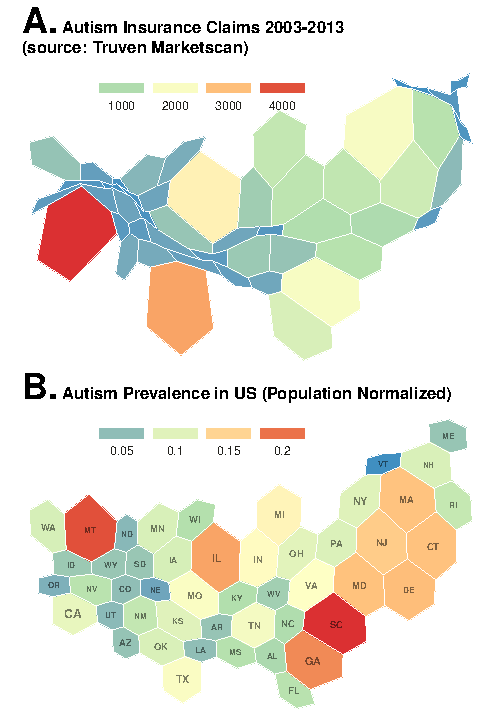
\includegraphics[width=0.8\textwidth]{Figures/External/occurv}

  \captionN{\textbf{ASD Occurrence Patterns}  Panel A illustrates the spatial distribution of ASD insurance claims, and panel B shows the same data after population normalization, illustrating the relatively small demographic skew to ASD prevalence within the general population with access to medical insurance, which is consistent with the suggestion that prevalence variation might be linked to regional and socioeconomic disparities in access to services~\cite{jarquin2011racial}.}\label{figocc}
    \vspace{-5pt}

\end{figure*}
%###########################################################
% ###########################################################
{\HCOL
\ifFIGS
\begin{figure*}[!ht]
  \centering
  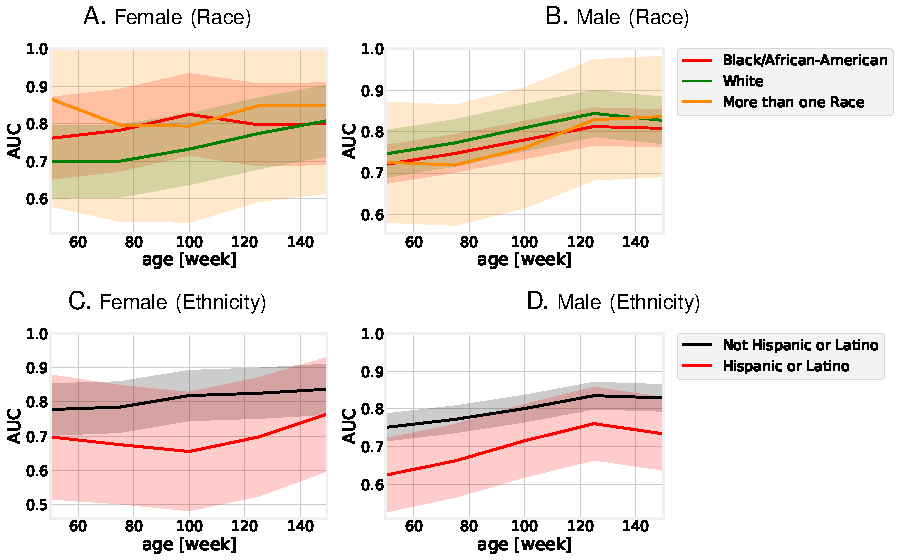
\includegraphics[width=\textwidth]{Figures/raceeth}

  \captionN{\HCOL \textbf{Effect of Race and Ethnicity on Predictive Performance with 95\% Confidence Bounds from the UCM dataset}. Panels A and B show the variation of AUC achieved in out-of-sample data in three race-based population groups (White, African-American anbd Multi-racial). We find no significant differences. Panels C and D show teh performance in Hispanic vs non-Hispanic sub-populations. We find that children with Hispanic backgound have a lower AUC, but the differences are not significant. Other races/ethnicities were not considered due to lack of sufficient data. }\label{figrace}
    \vspace{-5pt}

  \end{figure*}
  }
%###########################################################

\section{Detailed Mathematical Approach}\label{sec:mathdetails}
 
\subsection{Time-series Modeling of  Diagnostic History}
Individual diagnostic histories  can have long-term memory~\cite{ltgranger80}, implying that the order, frequency, and comorbid interactions between diseases are   important for assessing the future risk of our target phenotype. 
We analyze  patient-specific  diagnostic code sequences by first  representing the medical history of each patient as a set of stochastic categorical time-series | one each for a specific group of related disorders |  followed by the inference of stochastic models  for  these individual data streams. These inferred generators are from a special class of  Hidden Markov Models (HMMs), referred to as Probabilistic Finite State Automata (PFSA)~\cite{CL12g}. The inference algorithm we use is distinct from classical HMM learning, and has important advantages related to its ability to infer structure, and its sample complexity (See Supplementary text, Section~\ref{SI-sec:PFSA}). We infer a separate class of models for the \treatment and control cohorts, and then the problem reduces to determining the probability that the short diagnostic history from a  new  patient arises from the \treatment as opposed to the control category of the inferred models. 
%####################
\subsection{Step 1: Partitioning The Human Disease Spectrum}
We begin by partitioning the human disease spectrum into  $17$ non-overlapping  categories. Each category is defined by a set of diagnostic codes from the International Classification of Diseases, Ninth Revision (ICD9) (See  Table SI-\ref{SI-tab0} in the Supplementary text for description of  the categories used in this study). For this study, we considered $9,835$ distinct ICD9 codes (and their ICD10 General Equivalence Mappings (GEMS)~\cite{GEMS} equivalents). We came across 6,089 distinct ICD-9 codes and 11,522 distinct ICD-10 codes in total in the two datasets we analyzed. Transforming the diagnostic histories to report only the broad categories   reduces the number of distinct codes that the pipeline needs to handle, thus improving statistical  power.   
Our categories largely align with the top-level ICD9 categories, with small 
adjustments, $e.g.$ bringing all infections under one category irrespective of the pathogen or the target organ.
We do not pre-select the phenotypes; we want our algorithm to seek out the important patterns without any manual curation of the input data. The limitation of the set of phenotypes to $9835$ unique codes arises from excluding patients from the database who have very few and rare codes that will skew the statistical estimates. As shown in Table~\ref{main-tab2} in the main text, we exclude a very small number of patients, and who have  very short diagnostic histories with a very small number of codes.

% Next, we process raw diagnostic histories to  report only the categories. 
For each patient, the past  medical history is a sequence $(t_1,x_1),\cdots,(t_m,x_m)$, where $t_i$ are timestamps and $x_i$ are ICD9 codes diagnosed at time $t_i$.  We map individual patient history to a three-alphabet categorical time series $z^k$ corresponding to the disease category $k$,  as follows. For each week $i$, we have: 
\cgather{\label{eq1}
  z^k_i =  \left \{ \begin{array}{ll}
                      0 & \textrm{if no diagnosis codes  in week } i\\
                      1 & \textrm{if there exists a diagnosis of category $k$ in week } i\\
                      2 & \textrm{otherwise}
                    \end{array} \right.
                }\noindent
                The time-series $z^k$ is terminated at a particular week if the patient is diagnosed with ASD the week after. Thus for patients in the control cohort, the length of the mapped trinary series is limited by the time for which the individual is observed within the  2003 -- 2012 span of our database. In contrast, for patients in  the \treatment cohort, the length of the mapped series reflect the time to the first ASD diagnosis. Patients do not necessarily enter the database at birth, and we prefix each series with 0s to  approximately synchronize observations to age in weeks. Each patient is now represented by $17$ mapped trinary series.
                % ####################
                % %###########################################################
% % ###########################################################
\ifFIGS
\begin{figure*}[!t]
  \tikzexternalenable
    \tikzsetnextfilename{pfsa}
  \centering  
  \vspace{-10pt}
  
 \def\DATA{../../data_latest}
\iftikzX
\tikzstyle{stateM} = [
	circle, 
	draw=black, 
	fill=black, 
	minimum size=8,very thick
]
\tikzstyle{stateF} = [
	circle, 
	draw=Orchid2, 
	fill=Orchid!60, 
	minimum size=8,very thick
]
\tikzset{
    edge/.style={
        % decoration={
        %     markings,
        %     mark=at position #1 with {\arrow{>}}
        % },
		->,
		>=latex',
        postaction={decorate},
        draw=black,
		% font=\scriptsize,
        text=black,%MidnightBlue,
        thick
    }
}

\def\SCALE{.75}
\begin{tikzpicture}[font=\sffamily\fontsize{9}{10}\selectfont,text=black]
\def\FPATH{Figures/}
\def\PHN{digestive}
\def\XST{2.20in}
\def\YST{-.52in}
\def\Male{\bf\sffamily\large Male}
\def\Female{\bf\sffamily\large Female}
\node[scale=\SCALE,anchor=center] (xA) at (0,0) {\input{\FPATH/\PHN_female_c.tex}};
\node[scale=\SCALE,anchor=west] (xB) at ([xshift=\XST]xA.east) {\input{\FPATH/\PHN_female_p.tex}};
 \node[scale=\SCALE,anchor=north] (xC) at ([yshift=\YST]xA.south) {\input{\FPATH/\PHN_male_c.tex}};
 \node[scale=\SCALE,anchor=west] (xD) at ([xshift=-0.05in]$(xC.east)!(xB.west)!(xC.west)$) {\input{\FPATH/\PHN_male_p.tex}};
\draw[semithick,dashed,lightgray] ([xshift=-.75in]$(xA.west)!.6!(xC.west)$) -- ++(6.5in,0) node [rotate=90,fill=white,font=\bf\sffamily\LARGE] {\PHN};
\draw[very thick,black] ([yshift=-.12in]$(current bounding box.north west)!(xC.south west)!(current bounding box.south west)$) -- ([yshift=-.12in]$(current bounding box.north east)!(xC.south west)!(current bounding box.south east)$);

\node[anchor=south] (L1) at ([yshift=.45in]xA.north) {\Large \bf \sffamily Control};
\node[anchor=south] (L2) at ($(L1.south east)!(xB.north)!(L1.south west)$) {\Large  \bf \sffamily Positive};

\node[anchor=west] (L3) at ([xshift=.275in]xB.east) {\Female};
\node[anchor=west] (L4) at ($(L3.north west)!(xD.east)!(L3.south west)$) {\Male};

\draw[ultra thick,black] ([yshift=1.7in]$(current bounding box.north west)!(xC.south west)!(current bounding box.south west)$) -- ([yshift=1.7in]$(current bounding box.north east)!(xC.south west)!(current bounding box.south east)$);



\def\PHN{infectious}
\def\YST{-.15in}
\def\XST{.85in}

\node[scale=\SCALE,anchor=north] (xA) at ([xshift=.3in,yshift=\YST]xC.south) {\input{\FPATH/\PHN_female_c.tex}};
\node[scale=\SCALE,anchor=west] (xB) at ([xshift=\XST]xA.east) {\input{\FPATH/\PHN_female_p.tex}};
 \node[scale=\SCALE,anchor=north] (xC) at ([yshift=\YST]xA.south) {\input{\FPATH/\PHN_male_c.tex}};
 \node[scale=\SCALE,anchor=west] (xD) at ([xshift=-.75in]$(xC.east)!(xB.west)!(xC.west)$) {\input{\FPATH/\PHN_male_p.tex}};
\draw[semithick,dashed,lightgray] ([xshift=-.15in]$(xA.west)!.45!(xC.west)$) -- ++(6.5in,0) node [rotate=90,fill=white,font=\bf\sffamily\LARGE] {\PHN};
\draw[very thick,black] ([yshift=-.11in]$(current bounding box.north west)!(xC.south west)!(current bounding box.south west)$) -- ([yshift=-.11in]$(current bounding box.north east)!(xC.south west)!(current bounding box.south east)$);

\node[anchor=west] (L3) at ($(L3.north west)!(xB.east)!(L3.south west)$) {\Female};
\node[anchor=west] (L4) at ($(L3.north west)!(xD.east)!(L3.south west)$) {\Male};


\def\PHN{otic}
\def\YST{-.1in}
\def\XST{.85in}

\node[scale=\SCALE,anchor=north] (xA) at ([xshift=0in,yshift=\YST]xC.south) {\input{\FPATH/\PHN_female_c.tex}};
\node[scale=\SCALE,anchor=west] (xB) at ([xshift=\XST]xA.east) {\input{\FPATH/\PHN_female_p.tex}};
 \node[scale=\SCALE,anchor=north] (xC) at ([yshift=\YST]xA.south) {\input{\FPATH/\PHN_male_c.tex}};
 \node[scale=\SCALE,anchor=west] (xD) at ([xshift=-.75in]$(xC.east)!(xB.west)!(xC.west)$) {\input{\FPATH/\PHN_male_p.tex}};
\draw[semithick,dashed,lightgray] ([xshift=-.15in]$(xA.west)!.45!(xC.west)$) -- ++(6.5in,0) node [rotate=90,fill=white,font=\bf\sffamily\LARGE] {\PHN};
\draw[very thick,black] ([yshift=-.075in]$(current bounding box.north west)!(xC.south west)!(current bounding box.south west)$) -- ([yshift=-.075in]$(current bounding box.north east)!(xC.south west)!(current bounding box.south east)$);

\node[anchor=west] (L3) at ($(L3.north west)!(xB.east)!(L3.south west)$) {\Female};
\node[anchor=west] (L4) at ($(L3.north west)!(xD.east)!(L3.south west)$) {\Male};



\def\PHN{integumentary}
\def\YST{-.25in}
\def\XST{.85in}

\node[scale=\SCALE,anchor=north] (xA) at ([xshift=0in,yshift=\YST]xC.south) {\input{\FPATH/\PHN_female_c.tex}};
\node[scale=\SCALE,anchor=west] (xB) at ([xshift=\XST]xA.east) {\input{\FPATH/\PHN_female_p.tex}};
 \node[scale=\SCALE,anchor=north] (xC) at ([yshift=\YST]xA.south) {\input{\FPATH/\PHN_male_c.tex}};
 \node[scale=\SCALE,anchor=west] (xD) at ([xshift=-.75in]$(xC.east)!(xB.west)!(xC.west)$) {\input{\FPATH/\PHN_male_p.tex}};
\draw[semithick,dashed,lightgray] ([xshift=-.15in]$(xA.west)!.45!(xC.west)$) -- ++(6.5in,0) node [rotate=90,fill=white,font=\bf\sffamily\LARGE] {\PHN};
\draw[very thick,black] ([yshift=-.075in]$(current bounding box.north west)!(xC.south west)!(current bounding box.south west)$) -- ([yshift=-.075in]$(current bounding box.north east)!(xC.south west)!(current bounding box.south east)$);


\node[anchor=west] (L3) at ($(L3.north west)!(xB.east)!(L3.south west)$) {\Female};
\node[anchor=west] (L4) at ($(L3.north west)!(xD.east)!(L3.south west)$) {\Male};

% \def\PHN{integumentary}
% \def\YST{-.15in}
% \def\XST{.85in}

% \node[scale=\SCALE,anchor=north] (xA) at ([xshift=0in,yshift=\YST]xC.south) {\input{\FPATH/\PHN_female_c.tex}};
% \node[scale=\SCALE,anchor=west] (xB) at ([xshift=\XST]xA.east) {\input{\FPATH/\PHN_female_p.tex}};
%  \node[scale=\SCALE,anchor=north] (xC) at ([yshift=\YST]xA.south) {\input{\FPATH/\PHN_male_c.tex}};
%  \node[scale=\SCALE,anchor=west] (xD) at ([xshift=-.75in]$(xC.east)!(xB.west)!(xC.west)$) {\input{\FPATH/\PHN_male_p.tex}};
% \draw[semithick,dashed,lightgray] ([xshift=-.15in]$(xA.west)!.45!(xC.west)$) -- ++(6.5in,0) node [rotate=90,fill=white,font=\bf\sffamily\LARGE] {\PHN};

% \node[anchor=west] (L3) at ($(L3.north west)!(xB.east)!(L3.south west)$) {\Female};
% \node[anchor=west] (L4) at ($(L3.north west)!(xD.east)!(L3.south west)$) {\Male};


%\draw[very thick,black] ([yshift=-.15in]$(current bounding box.north west)!(xC.south west)!(current bounding box.south west)$) -- ([yshift=-.15in]$(current bounding box.north east)!(xC.south west)!(current bounding box.south east)$);




\draw[ultra thick,gray!20] ($(xC.south east)!1.1!(xD.south east)$) -- ++(0,7.95in);
\draw[ultra thick,gray!20] ($(xC.south east)!.5!(xD.south west)$) -- ++(0,7.95in);


\end{tikzpicture}

\else
  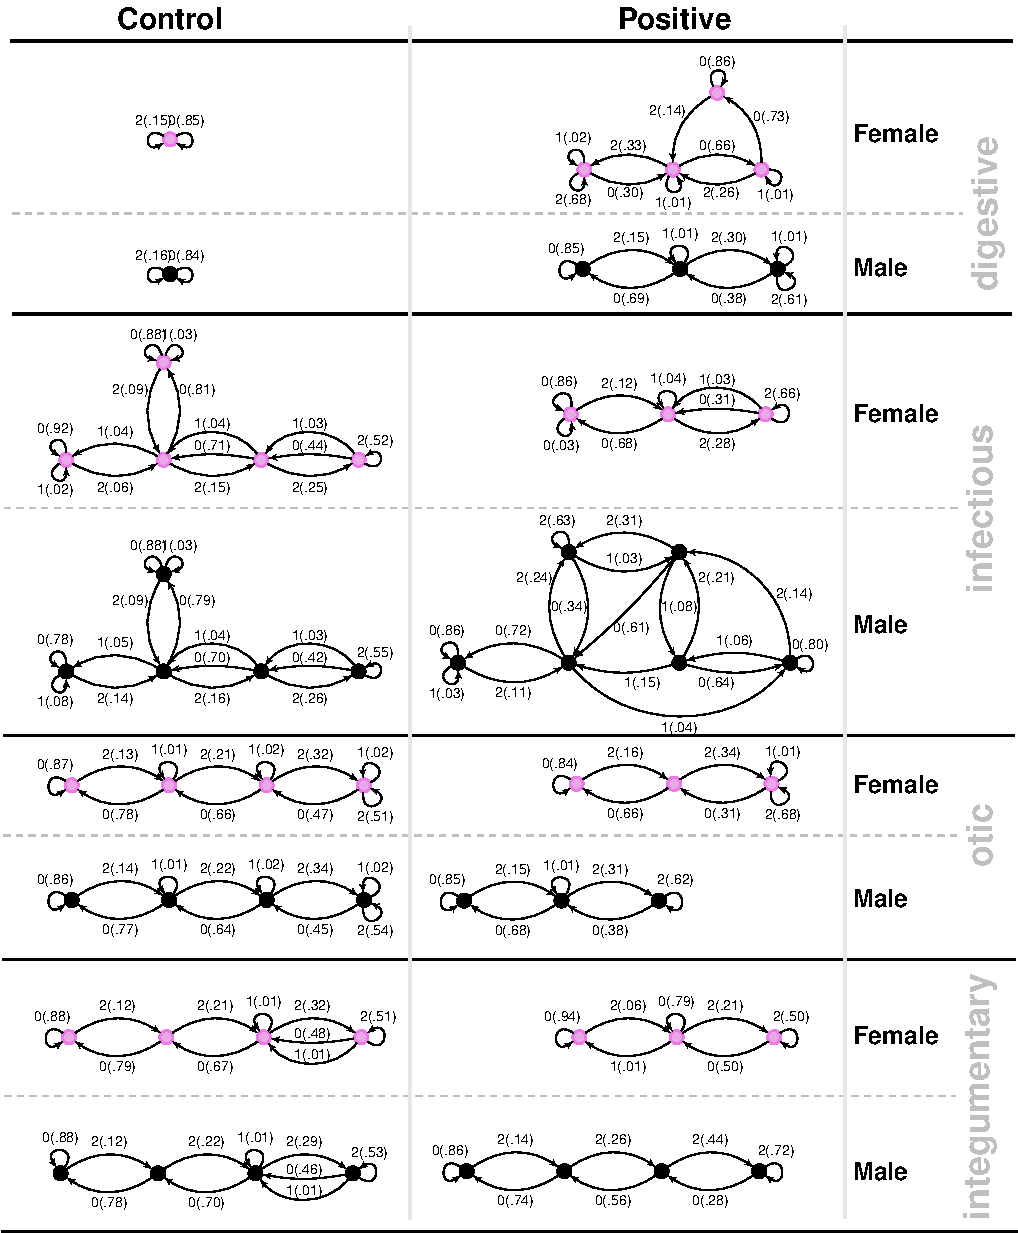
\includegraphics[width=0.95\textwidth]{Figures/External/pfsa}
  \fi
      \vspace{-5pt}

     \captionN{Probabilistic Finite State Automata models generated for different disease categories for the control and \treatment cohorts. We note that in the first  cases (digestive disorder), the models get more complex in the \treatment cohort, suggesting that the disorders become less random. However, in the categories of otic and integumentary disorders, the models become less complex suggesting increased independence from past events of similat nature. In case of infectious diseases, the model gets more complex for males, and less complex for females, suggesting distinct sex-specific responses associated with high ASD risk.}\label{EXT-autgrid}
\end{figure*}
\else
\refstepcounter{figure}\label{EXT-autgrid}
\fi
% ###########################################################

\subsection{Step 2: Model Inference \& The Sequence Likelihood Defect}
The mapped series, stratified by  sex, disease-category, and ASD diagnosis-status are considered to be independent sample paths, and we want to explicitly model these systems as specialized HMMs (PFSAs). We model the \treatment and the control cohorts for each sex, and in  each disease category separately, ending up with a total of $68$ HMMs at the population level ($17$ categories, $2$ sexes, $2$ cohort-types: \treatment and control, SI-Fig.~\ref{SI-EXT-autgrid} in the supplementary text provides some examples). Each of these inferred models is  a PFSA;  a directed graph with probability-weighted edges, and acts as an optimal generator of the  stochastic process driving the  sequential appearance of the three letters (as defined by Eq.~\eqref{eq1})  corresponding to each sex, disease category, and cohort-type (See Section~\ref{SI-sec:PFSA} in the Supplementary text for  background on PFSA inference). 

To reliably infer the cohort-type of a new patient, $i.e$, the likelihood of a diagnostic sequnce being generated by the corresponding cohort model, we generalize the notion of Kullbeck-Leibler (KL) divergence~\cite{Cover,kullback1951} between probability distributions to a divergence $\mathcal{D}_{\textrm{KL}}(G \vert \vert H)$ between ergodic stationary categorical stochastic processes~\cite{doob1953stochastic} $G,H$ as:
\cgather{
  \mathcal{D}_{\textrm{KL}}(G \vert \vert H) = \lim_{n\rightarrow \infty} \frac{1}{n}  \sum_{x:|x| = n}p_G(x)\log\frac{p_G(x)}{p_H(x)}  }%
where $\vert x\vert $ is the sequence length, and $p_G(x) ,p_H(x) $ are the probabilities of sequence $x$ being generated by the processes $G,H$ respectively. Defining the  log-likelihood of  $x$ being generated by a process $G$ as :
\cgather{
  L(x,G)= -\frac{1}{\vert x\vert}\log p_G(x) 
}%
The cohort-type for an observed sequence $x$ | which is actually generated by the hidden process $G$ | can be formally inferred from observations based on the following provable relationships (See Suppl. text Section~\ref{SI-sec:PFSA}, Theorem 6 and 7):
\begin{subequations}\label{eqR}\cgather{
    \lim_{\vert x \vert \rightarrow \infty}L(x,G) = \mathcal{H}(G)   \\
    \lim_{\vert x \vert \rightarrow \infty } L(x,H)  =\mathcal{H}(G) +  \mathcal{D}_{\textrm{KL}}(G \vert \vert H)   
  }\end{subequations}%
where  $\mathcal{H}(\cdot)$ is the entropy rate of a process~\cite{Cover}. Importantly, Eq.~\eqref{eqR} shows that the computed likelihood has an additional non-negative contribution from the divergence term when we choose the incorrect generative process.  Thus, if a  patient is eventually going to be diagnosed with ASD, then we expect that the disease-specific mapped series corresponding to  her diagnostic history be modeled by the PFSA in the \treatment cohort. Denoting the PFSA corresponding to disease category $j$ for \treatment and control cohorts as $G^{j}_+,G^{j}_0$ respectively, we can compute the \textit{sequence likelihood defect} (SLD, $\Delta^j$) as:
\cgather{
  \Delta^j \triangleq L(G^{j}_0,x) - L(G^{j}_+,x) \rightarrow \mathcal{D}_{\textrm{KL}}(G^{j}_0 \vert \vert G^{j}_+) \label{eq6}
}%
With  the inferred  PFSA  models and  the individual diagnostic history, we  estimate the SLD measure on the  right-hand side of Eqn.~\eqref{eq6}. The higher this likelihood defect, the higher  the similarity of diagnosis history to that of children with autism.
%####################
\subsection{Step 3: Risk Estimation Pipeline With Semi-supervised \& Supervised Learning Modules}
The risk estimation pipeline operates on patient specific information limited to the sex and available  diagnostic history from birth, and produces an estimate of the relative risk of ASD diagnosis at a specific age, with an associated  confidence value. To learn the parameters and associated model structures of  this pipeline, we transform the patient specific data to a set of engineered features, and the feature vectors realized on the
\treatment and control sets are  used to train a gradient-boosting classifier~\cite{friedman}. The complete list of $165$ features used  is provided in Tab.~\ref{main-EXT-tab1} in the main text.

We need two training sets: one to infer the models, and one to  train the classifier  with features  derived  from the inferred models. Thus, we do a random 3-way split of the set of unique patients into \textit{feature-engineering} ($25\%$), \textit{training} ($25\%$) and \textit{test} ($50\%$) sets. We use the feature-engineering set of ids first to infer our PFSA models \textit{(unsupervised model inference in each category)}, which then allows us to train the gradient-boosting classifier using the training set and PFSA models \textit{(classical supervised learning)}, and we finally execute  out-of-sample validation on the test set. Fig.~\ref{main-fig1}B in the main text shows the top $15$ features  ranked in order of their relative importance (relative loss in performance when dropped out of the analysis). 
\section{Comparison With State of the Art Off-the-shelf ML Algorithms}\label{sec:offtheshelf}
%###########################################################
%###########################################################
%###########################################################
 {\NCOL \begin{figure}[!ht]
    \begin{verbatim}
Model: "sequential_4"
_________________________________________________________________
Layer (type)                 Output Shape              Param #   
=================================================================
lstm_1 (LSTM)                (None, 150)               180600    
_________________________________________________________________
dense_5 (Dense)              (None, 32)                4832      
_________________________________________________________________
dense_6 (Dense)              (None, 1)                 33        
=================================================================
Total params: 185,465
Trainable params: 185,465
Non-trainable params: 0
_________________________________________________________________
\end{verbatim}
    \captionN{\HCOL The simplest LSTM investigated as a baseline. More complex models have significantly larger number of trainable parameters (1 to 10 Million). In contrast our pipeline has 13,744 trainable parameters.}\label{figlstmex}
\end{figure}
}

Off the shelf algorithms with little or no pre-processing, $i.e.$, using the diagnostic codes themselves are time-stamped categorical features failed to produce clinically relevant performance (See SI-Fig.~\ref{EXT-figcompwsoa}). Classifiers such as random forests~\cite{breiman}, and gradient boosters~\cite{friedman} might be penalized due to their inability to take into account long-range temporal information. Since the number of diagnostic codes available per patient is small, recurrent neural network implementations such as LSTM~\cite{hochreiter} might be suffering from the data sparsity in training. It is possible that the performance of the competing approaches might be improved with extensive tuning or clever feature-engineering.
%###########################################################
%###########################################################
%###########################################################
\section{Comparison With  Pipeline Variations, Feature Subsets and Neural Net Post-processing}\label{sec:pipelinevar}
In addition to the naive baseline approaches, we also evaluated the performance achievable  with LSTMs (denoted as LSTMB in SI-Fig.~\ref{EXT-figcompwsoa}) that use identical preprocessing as our pipeline, $i.e.$, representation of diagnostic histories as trinary sequences in 18 categories for each patient, and achieved $\sim$80\% AUC  at 150 weeks for males in the Truven database (compared to $> 85\%$ for our approach). However, the performances drop significantly when the number of positive samples is reduced, yielding an AUC of 66\% on the UCM dataset for males, 60\% for females on the Truven dataset, and a  worse-than-random 40\% on the UCM dataset respectively (See Fig.~\ref{EXT-figcompwsoa}). 

  Much better results were obtained when we compared our optimized pipeline to pipelines that use only a subset of our features: namely, the  ones that use only features derived from sequence statistics and exclude the ones derived from learning PFSAs (recall that PFSAs are special HMMs we learn using our novel algorithms)  from the disease categories as described in Methods in the main text, or using only the PFSA-based SLD features, or using simply the density of diagnostic codes (See Fig.~\ref{EXT-figcompsi}, panel D). In all these cases we analyzed, our pipeline has a clearly demonstrable advantage (See  Fig.~\ref{EXT-figcompsi}, panel D) that is stable across databases,  under reductions in sample sizes, and in balanced resampling experiments (See Fig.~\ref{EXT-figcompsi}, panel C).
  
 {\HCOL While it is difficult to explain the exact source of a modeling framework's performance, and even more difficult to explain  non-performance, we can point to the following advantages that our approach has over existing techniques:}
  \begin{enumerate}\HCOL
    \item \textbf{Purely Classification Algorithms With No Pre-processing Do not Do well.} Pure classifiers such as random forests, gradient boosters, etc. are not time series modeling frameworks, and might not capture stochastic temporal patterns well. While features are not certainly assumed to be independent in these algorithms, it is problematic to learn patterns that do not appear at fixed time points in the diagnostic history.
  \item \textbf{Lower Sample Complexity Compared to Deep Learning Frameworks.} Compared to LSTMs and RNNs, we are able to capture stochastic behavior with more compact models, which results in  better sample complexity. In other words, if we have less data, our models do better, because we estimate fewer parameters.
  \item \textbf{Designed Bottom-up for Learning Stochastic Processes.} It is easily demonstrated that LSTMs and RNNs, while good models of complicated time series in many cases, do not work well for data that are generated by stochastic processes, $i.e.$ are sample paths of a hidden process.
    % \item \textbf{We May Have  Missed Some Clever Transformation.} It is possible that extensive tuning or feature selection with LSTMs, RNNs or CNNs or some combination thereof, can replicate our performance, or even do better. There will always be that possibility, notwithstanding how much effort we put in to evaluate competing techniques. The authors welcome  \textit{future work in this direction that surpasses our  performance reported here; this  is only going to help the patients  which is what  matters.}
  \end{enumerate}
  %

  {\HCOL
  Thus, there are two key and related issues:  NN models generally have a relatively large number of parameters, and  these large number of trainable parameters require substantial amount of data to train. In our case, we indeed have a large number of control examples, but a relatively smaller number of positive examples (children who get diagnosed with autism eventually). The amount of training data, even with our large patient database, is not enough to train anything but the simplest of the NN architectures, and even then the number of parameters for such NN models is substantially larger compared to our architecture. This is shown in our example (See SI-Fig.~\ref{figlstmex}), where one of the LSTM models we investigate (the simplest one we tested) has 185,465 parameters, whereas our complete end to end pipeline has 7025+6719=13,744 trainable parameters (an order of magnitude less, where the first contribution is from inferred PFSA models, the second from the ensemble of decision trees in the final gradient boosting model). Additionally, the number of parameters for deep learning models rapidly increase to millions or tens of millions as the models get more complicated.

 Also note that our framework is adaptive (See examples of PFSA models inferred in SI-Fig.~\ref{EXT-autgrid}), and the network structures of the inferred PFSA models is inferred from data, and not fixed a priori; it produces more states where it needs, thus adapting the model resolution to more complex contexts, and obtaining significantly more compact yet effective representations. We must however add the caveat that with sufficient patience and experience it might be possible to devise a specific NN architecture with similar performance to our framework; however, in our approach such artful insight is unnecessary. 

It also seems possible that NN models, which have no stochastic parameters or components, generalize poorly in this context, which is why the performance is relatively better in the Truven dataset (See SI-Fig.~\ref{EXT-figcompwsoa}), but worse in an independent database.
}
%####################
%###########################################################
\ifFIGS
\begin{figure}[t]
  \tikzexternalenable 
    \tikzsetnextfilename{stdtools}
    \def\TEXTCOL{gray}
    \def\MXCOL{black}
    \centering

   \iftikzX
  \begin{tikzpicture}[font=\bf\sffamily\fontsize{8}{8}\selectfont]
    \def\DATA{Figures/comp.csv}
    \def\WDT{3in}
    \def\HGT{2in}
 \def\AXISCOL{white}
  \def\MXCOLB{lightgray}
  \def\FXCOLB{CadetBlue2}
  \def\BANDCOL{lightgray}
  \def\PLOTCOLA{black}
  \def\PLOTCOLB{\MXCOL}
  \def\PLOTCOLBu{\MXCOL}
  \def\PLOTCOLC{black}
  \def\PLOTCOLD{\FXCOL}
  \def\FNCOLB{SeaGreen2}
  \def\PLOTCOLDu{\FXCOL}
  \def\WDTa{2.2in}
  \def\HGTa{1.850in}
\def\OPC{.9}
    \def\SKIP{4}

\def\datafilemt{../../../revision_results/LSTM_comparison/truven_male.csv}
\def\datafilemu{../../../revision_results/LSTM_comparison/ucm_male.csv}
\def\datafileft{../../../revision_results/LSTM_comparison/truven_female.csv}
\def\datafilefu{../../../revision_results/LSTM_comparison/ucm_female.csv}
\def\LWDT{.5mm}
  
    \node[] (A) at (0,0) {
        \begin{tikzpicture}[font=\bf\sffamily\fontsize{8}{8}\selectfont]
    \begin{axis}[legend cell align=left,legend style={anchor=west,at={(.1,0.8)},inner sep=3pt,draw=none,fill=white,fill opacity=.85,align=right,text opacity=1,font=\bf\sffamily\fontsize{8}{9}\selectfont},axis line style={lightgray, opacity=0.50, thin},%
      enlargelimits=true,
      % grid,
      xshift=.1in,
      anchor=north west,
      height=\HGT,
      width=\WDT,
      ybar, 
      xtick=data,% crucial line for the xticklabels directive 
      xmin=0, 
      xticklabels from table={\DATA}{algorithm},
      xticklabel style={font=\bf\sffamily\fontsize{7}{7}\selectfont,align=right,rotate=90,  anchor=east, yshift=0in,xshift=-0.1in,text=\TEXTCOL},
      major tick length=0pt,
      yticklabel style={font=\bf\sffamily\fontsize{7}{7}\selectfont,text=\TEXTCOL},
      grid,
      grid style={lightgray, opacity=.7},xlabel={algorithm},
      axis on top=false, bar width=15pt,ylabel={AUC},xlabel style={yshift=-0.750in,text=\TEXTCOL},
      %enlarge y limits=0.03,
      ] 

      \addplot[opacity=1,fill=\MXCOL, area legend] table [ 
      x expr=\coordindex,
      y=AUC
      ] {\DATA};   
      %\addlegendentry{Male (sample size: 300K)}

    \end{axis} 
  \end{tikzpicture}};
\node[anchor=south west] (B) at ([xshift=0.2in]A.south east) {
  \begin{tikzpicture}
    \begin{axis} [,legend cell align={left},
      legend style={anchor=east,at={(0,.97)},
        inner sep=3pt,
        draw=none,
        fill=white,fill opacity=.850,
        align=left,anchor=west,
        text opacity=1,
        font=\bf\sffamily\fontsize{8}{9}\selectfont,text=black},
      grid style={thick,dashed, gray!40},
      grid,
      enlargelimits=true,scale only axis=true,
      scaled x ticks = false,scaled y ticks = false,
      height=\HGTa,
      width=\WDTa,
      ,axis line style={\AXISCOL, opacity=1,ultra  thick, rounded corners=0pt}, y tick label style={/pgf/number format/fixed,/pgf/number format/precision=1,/pgf/number format/fixed zerofill,
        /pgf/number format/1000 sep = %\thinspace % Optional if you want to replace comma as the 1000 separator 
      },
      major tick length=0pt,legend columns=2, legend style={,xshift=-.5in,yshift=.2in},
      yshift=-.75in,text=\TEXTCOL,xlabel={FPR},xlabel style={yshift=0.025in},ylabel
      style={xshift=-0.1in},ylabel={TPR},
      grid style={thick,dashed, gray!40},xmin=-.050]
      
      \addplot[ each nth point=\SKIP, filter discard warning=false, 
        unbounded coords=discard,smooth,smooth,  line width=\LWDT, \MXCOL,mark=none, opacity=\OPC,
      ]table[col sep=comma,x=fpr, y=tpr]
      {\datafilemt};
      \addlegendentry{Males (Truven)}


      \addplot[ each nth point=\SKIP, filter discard warning=false, 
        unbounded coords=discard,smooth,smooth,  line width=\LWDT, \FXCOL,mark=none, opacity=\OPC,
      ]table[col sep=comma,x=fpr, y=tpr]
      {\datafileft};
      \addlegendentry{Females (Truven)}      

      \addplot[ each nth point=\SKIP, filter discard warning=false, 
        unbounded coords=discard,smooth,smooth,  line width=\LWDT, \MXCOLB,mark=none, opacity=\OPC,
      ]table[col sep=comma,x=fpr, y=tpr]
      {\datafilemu};
      \addlegendentry{Males (UCM)}

      \addplot[ each nth point=\SKIP, filter discard warning=false, 
        unbounded coords=discard,smooth,smooth,  line width=\LWDT, \FXCOLB,mark=none, opacity=\OPC,
      ]table[col sep=comma,x=fpr, y=tpr]
      {\datafilefu};
      \addlegendentry{Females (UCM)}

      \draw[fill=lightgray,draw=none,opacity=.5] (axis cs:0,0) -- (axis cs:1,0) -- (axis cs:1,1) -- cycle;
    \end{axis}
  \end{tikzpicture}
};
\node[anchor=south west] (L1) at (A.north west) {{\Large A.} Sample of Baseline Approaches with AUC $>0.5$ };
\node[anchor=south west] (L2)  at ($(L1.south west)!(B.west)!(L1.south east)$) {{\Large B.} ROC Curves for LSTMB (LSTM with pre-processing)};

\end{tikzpicture}
\else
  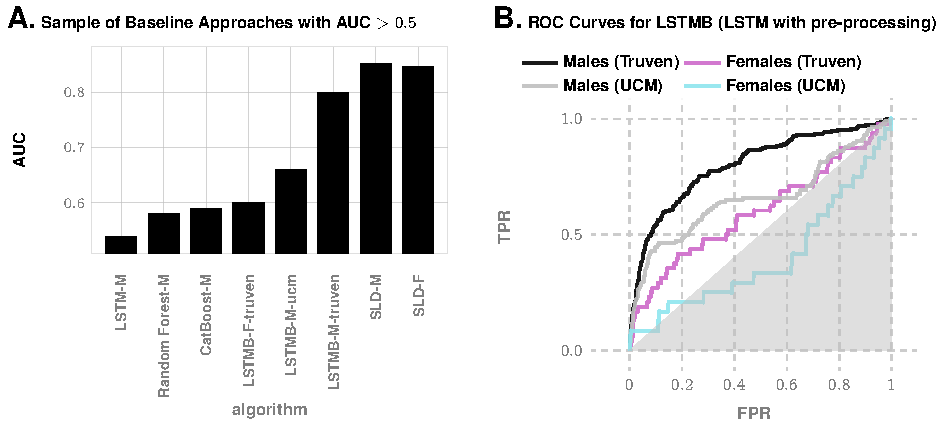
\includegraphics[width=0.9\textwidth]{Figures/External/stdtools}
  \fi 
  \captionN{Performance of standard tools on correctly predicting eventual ASD diagnosis, computed at age $150$ weeks of age. Long-short Term Memory (LSTM) networks are the state of the art variation of recurrent neural nets, and Random Forests and Gradient Boosting classifiers (CatBoost) are generally regarded as a representative state of the art classification algorithms. Sequence Likelihood Defect (SLD) is the approach developed in this study. LSTMB denotes LSTM with identical pre-processing as in our pipeline (instead of using raw diagnostic codes). We get much better performance with LSTMB with males in the Truven dataset, but the performance is sensitive to the sizes of the training set, and degrades for smaller samples available for females and in the UCM database, as shown in Panel B.}\label{EXT-figcompwsoa}
\end{figure}
\else
\refstepcounter{figure}\label{EXT-figcompwsoa}
\fi
%###########################################################
%###########################################################
%###########################################################
\ifFIGS
\begin{figure*}[!ht]
  \tikzexternalenable
    \tikzsetnextfilename{sanitycheck}
  \vspace{-10pt}
  
  \centering
\iftikzX
\pgfplotsset{
  discard if/.style 2 args={
    x filter/.append code={
      \edef\tempa{\thisrow{#1}}
      \edef\tempb{#2}
      \ifx\tempa\tempb
      \def\pgfmathresult{inf}
      \fi
    }
  },
  discard if not/.style 2 args={
    x filter/.append code={
      \edef\tempa{\thisrow{#1}}
      \edef\tempb{#2}
      \ifx\tempa\tempb
      \else
      \def\pgfmathresult{inf}
      \fi
    }
  }
}

\begin{tikzpicture}[font=\bf\sffamily\fontsize{8}{10}\selectfont]
  \def\TEXTCOL{gray}
  \tikzset{
    hatch distance/.store in=\hatchdistance,
    hatch distance=20pt,
    hatch thickness/.store in=\hatchthickness,
    hatch thickness=2pt
  }

  \def\WDT{4.75in} 
  \def\WDTA{2in}
  
\def\DATA{../../data_revision}
\def\DATAPATH{/home/ishanu/ZED/Research/XG3_/autism/revision_results/performance/restricted_neg_len/} 
\def\datafile{\DATAPATH/PERFORMANCE_STATS.csv}
\def\datafileE{\DATAPATH/equal_size_auc/sample_auc_stats.csv}
\def\datafileEmt{\DATAPATH/equal_size_auc/male_truven.csv}
\def\datafileEft{\DATAPATH/equal_size_auc/female_truven.csv}
\def\datafileEmu{\DATAPATH/equal_size_auc/male_UCM.csv}
\def\datafileEfu{\DATAPATH/equal_size_auc/female_UCM.csv}
  \def\auctime{\DATA/figfiles/auc_time.csv}
  \def\auctimeV{\DATA/figfiles/Vauc_time.csv}

  \def\HGT{1.6in}
  \def\WDT{1.25in}
  \def\WDTC{4in}
  \def\WDTR{1.9in}
  \def\WDTH{1.7in}

\def\MXCOLX{DarkOrange1}
\def\FXCOLX{SeaGreen4}

  \def\AXISCOL{white}
  \def\MXCOLB{lightgray}
  \def\FXCOLB{CadetBlue2}
  \def\BANDCOL{lightgray}
  \def\PLOTCOLA{black}
  \def\PLOTCOLB{\MXCOL}
  \def\PLOTCOLBu{\MXCOL}
  \def\PLOTCOLC{black}
  \def\PLOTCOLD{\FXCOL}
  \def\FNCOLB{SeaGreen2}
  \def\PLOTCOLDu{\FXCOL}
  \def\WDTa{1.85in}
  \def\HGTa{2in}

  \def\SCALE{1.5}
  \def\SCALEA{1.25}
  \def\SCALEB{1.15}
  \def\SCALEX{1.5}
  \def\OPC{.55}
  \def\OPCh{.55}
  \def\OPCX{.65}
  \def\OPCB{.65}
  \def\BWIDTH{4pt}
  \def\LWDT{0.5mm}
  \def\LWDTX{1mm}
  \node[] (A0) at (0,0) {};

  \node[anchor=center] (N) at (A0.south)
  {
    \begin{tikzpicture}
      \begin{axis} [,legend cell align={left},
        legend style={anchor=east,at={(0.25,1.1)},
          inner sep=3pt,
          draw=none,
          fill=white,fill opacity=.850,
          align=left,anchor=west,
          text opacity=1,
          font=\bf\sffamily\fontsize{8}{9}\selectfont,text=black},
        grid style={thick,dashed, gray!40},
        grid,
        enlargelimits=true,scale only axis=true,
        scaled x ticks = false,scaled y ticks = false,
        height=\HGTa,
        width=\WDT,
        enlarge x limits=0.07,axis line style={\AXISCOL, 
          opacity=1,ultra  thick, rounded corners=0pt}, 
        y tick label style={/pgf/number format/fixed,
          /pgf/number format/precision=2,/pgf/number format/fixed zerofill,
          /pgf/number format/1000 sep = %\thinspace % Optional 
        },
        major tick length=0pt,legend columns=1, legend style={,xshift=-.5in,yshift=.2in},
        yshift=-.75in,text=\TEXTCOL,xlabel={age [weeks]},xlabel style={yshift=0.025in},ylabel
        style={xshift=-0in},ylabel={AUC},
        grid style={thick,dashed, gray!40},
        % ymax=0.855
        ]
        
        \draw [draw=none,ultra thick,opacity=.2,postaction={
          pattern=flexible hatch,
          hatch distance=7pt,
          hatch thickness=2pt,
          draw=none,
          opacity=.5,
          pattern color=lightgray, %ultra thick,
        },] (axis cs:150,\pgfkeysvalueof{/pgfplots/ymin})
        -- (axis cs:150,\pgfkeysvalueof{/pgfplots/ymax}) -- 
        (axis cs:100,\pgfkeysvalueof{/pgfplots/ymax}) 
        -- (axis cs:100,\pgfkeysvalueof{/pgfplots/ymin}) --cycle;

        \addplot[ smooth,  line width=\LWDT, \PLOTCOLB,mark=*, opacity=\OPC,
        mark options={%
          scale=\SCALEB,draw=\PLOTCOLB,  thick, fill=\PLOTCOLB,  
          opacity=\OPC,
        },]table[col sep=comma,x=week, y=auc, 
        discard if not={dataset}{pipeline},
        discard if not={tag}{PSYCH},,discard if not={gender}{M}]
        {\datafile};
        \addlegendentry{Males (Truven)}
        % 
        \addplot[ smooth,  line width=\LWDT, \PLOTCOLD,mark=*, opacity=\OPC,
        mark options={%
          scale=\SCALEB,draw=\PLOTCOLD,  thick, fill=\PLOTCOLD,  opacity=\OPC,
        },]table[col sep=comma,x=week, y=auc, 
        discard if not={dataset}{pipeline},
        discard if not={tag}{PSYCH},,discard if not={gender}{F}]
        {\datafile};
        \addlegendentry{Females (Truven)}
        % 
      \end{axis}\end{tikzpicture}
  };
  \node[anchor=south west] (N1) at (N.south east)
  {
    \begin{tikzpicture}
      \begin{axis} [,legend cell align={left},
        legend style={anchor=east,at={(0,1.1)},
          inner sep=3pt,
          draw=none,
          fill=white,fill opacity=.850,
          align=left,anchor=west,
          text opacity=1,
          font=\bf\sffamily\fontsize{8}{9}\selectfont,text=black},
        grid style={thick,dashed, gray!40},
        grid,
        enlargelimits=true,scale only axis=true,
        scaled x ticks = false,scaled y ticks = false,
        height=\HGTa,
        width=\WDT,
        enlarge x limits=0.07,axis line style={\AXISCOL, opacity=1,
          ultra  thick, rounded corners=0pt}, 
        y tick label style={/pgf/number format/fixed,
          /pgf/number format/precision=2,/pgf/number format/fixed zerofill,
          /pgf/number format/1000 sep = %\thinspace % 
        },
        major tick length=0pt,legend columns=1, legend style={,xshift=-.5in,yshift=.2in},
        yshift=-.75in,text=\TEXTCOL,xlabel={age [weeks]},xlabel style={yshift=0.025in},ylabel
        style={xshift=-0in},ylabel={},
        grid style={thick,dashed, gray!40},
        % ymax=0.855
        ]
        
        \draw [draw=none,ultra thick,opacity=.2,postaction={
          pattern=flexible hatch,
          hatch distance=7pt,
          hatch thickness=2pt,
          draw=none,
          opacity=.5,
          pattern color=lightgray, %ultra thick,
        },] (axis cs:150,\pgfkeysvalueof{/pgfplots/ymin}) 
        -- (axis cs:150,\pgfkeysvalueof{/pgfplots/ymax}) 
        -- (axis cs:100,\pgfkeysvalueof{/pgfplots/ymax}) 
        -- (axis cs:100,\pgfkeysvalueof{/pgfplots/ymin}) --cycle;

        \addplot[ smooth,  line width=\LWDT, \PLOTCOLB,mark=*, opacity=\OPC,
        mark options={%
          scale=\SCALEB,draw=\PLOTCOLB,  thick, fill=\PLOTCOLB,  opacity=\OPC,
        },]table[col sep=comma,x=week, y=auc, discard if not={dataset}{pipeline},
        discard if not={tag}{TWOTARG},,discard if not={gender}{M}]
        {\datafile};
        \addlegendentry{Males (Truven, two codes)}
        % 
        \addplot[ smooth,  line width=\LWDT, \PLOTCOLD,mark=*, opacity=\OPC,
        mark options={%
          scale=\SCALEB,draw=\PLOTCOLD,  thick, fill=\PLOTCOLD,  
          opacity=\OPC,
        },]table[col sep=comma,x=week, y=auc, 
        discard if not={dataset}{pipeline},discard if not={tag}{TWOTARG},,
        discard if not={gender}{F}]
        {\datafile};
        \addlegendentry{Females (Truven, two codes)}
        % 

        \addplot[ smooth,  line width=\LWDT, \PLOTCOLB,mark=square*, opacity=\OPCB,
        mark options={%
          scale=\SCALEA,draw=\PLOTCOLB,  thick, fill=\PLOTCOLB,  opacity=\OPCB,
        },]table[col sep=comma,x=week, y=auc, discard if not={dataset}{pipeline},
        discard if not={tag}{BASIC},,discard if not={gender}{M}]
        {\datafile};
        \addlegendentry{Males (Truven, one code)}
        % 
        \addplot[ smooth,  line width=\LWDT, \PLOTCOLD,mark=square*, opacity=\OPCB,
        mark options={%
          scale=\SCALEA,draw=\PLOTCOLD,  thick, fill=\PLOTCOLD,  opacity=\OPCB,
        },]table[col sep=comma,x=week, y=auc, discard if not={dataset}{pipeline},
        discard if not={tag}{BASIC},,discard if not={gender}{F}]
        {\datafile};
        \addlegendentry{Females (Truven, one code)}
        % 
      \end{axis}\end{tikzpicture}
  };

  \node[anchor=south west] (N1c) at (N1.south east)
  {
    \begin{tikzpicture}
      \begin{axis} [,legend cell align={left},
        legend style={anchor=east,at={(0,1.1)},
          inner sep=3pt,
          draw=none,
          fill=white,fill opacity=.850,
          align=left,anchor=west,
          text opacity=1,
          font=\bf\sffamily\fontsize{8}{9}\selectfont,text=black},
        grid style={thick,dashed, gray!40},
        grid,
        enlargelimits=true,scale only axis=true,scaled x ticks = false,
        scaled y ticks = false,
        height=\HGTa,
        width=\WDTa,
        enlarge x limits=0.07,axis line style={\AXISCOL, opacity=1,ultra  thick, 
          rounded corners=0pt}, y tick label style={/pgf/number format/fixed,
          /pgf/number format/precision=2,/pgf/number format/fixed zerofill,
          /pgf/number format/1000 sep = %\thinspace % Optional 
        },
        major tick length=0pt,legend columns=1, 
        legend style={,xshift=-.5in,yshift=.2in},
        yshift=-.75in,text=\TEXTCOL,xlabel={AUC},
        xlabel style={yshift=0.025in},
        ylabel
        style={xshift=-0.4in},ylabel={histogram bin count},
        grid style={thick,dashed, gray!40},
        % ymax=0.855
        ]

        \addplot[draw=gray,fill  opacity=.4,fill=\MXCOL,area legend,hist={
        bins=10,%,density=true,
        data min=0.77,
        data max=.87,%handler/.style={sharp plot},
  %intervals=false
      }   ]table[col sep=comma,y index=3, 
        ]
        {\datafileEmt};
        \addlegendentry{Males (Truven)}

        \addplot[draw=gray, fill opacity=\OPCh,fill=\FXCOL,area legend,hist={
        bins=12,%density=true,
        data min=0.78,
        data max=.87,%handler/.style={sharp plot},
        %intervals=false
      }   ]table[col sep=comma,y index=3, 
        ]
        {\datafileEft};
        \addlegendentry{Females (Truven)}

        \addplot[draw=gray, fill opacity=\OPCh,fill=\MXCOLB,area legend,hist={
        bins=10,%,density=true,
        data min=0.78,
        data max=.89,
        % handler/.style={sharp plot},
        %intervals=false
      }   ]table[col sep=comma,y index=3, 
        ]
        {\datafileEmu};
        \addlegendentry{Males (UCM)}

        \addplot[draw=gray, fill opacity=\OPCh,fill=\FXCOLB,area legend,hist={
        bins=6,
        % ,density=true,
        data min=0.8,
        data max=.85,
        % handler/.style={sharp plot,smooth},
        % intervals=false
      }   ]table[col sep=comma,y index=3, 
        ]
        {\datafileEfu};
        \addlegendentry{Females (UCM)}

      \end{axis}\end{tikzpicture}
  };

  \node[anchor=north west] (N2) at ([yshift=-.45in]N.south west)
  {
    \begin{tikzpicture}
      \begin{axis} [,legend cell align={left},
        legend style={anchor=east,at={(1.4,.35)},
          inner sep=3pt,
          draw=none,
          fill=white,fill opacity=.850,
          align=left,anchor=west,
          text opacity=1,
          font=\bf\sffamily\fontsize{8}{9}\selectfont,text=black},
        grid style={thick,dashed, gray!40},
        grid,
        enlargelimits=true,scale only axis=true,scaled x ticks = false,
        scaled y ticks = false,
        height=\HGTa,
        width=\WDTa,
        enlarge x limits=0.07,axis line style={\AXISCOL, opacity=1,
          ultra  thick, 
          rounded corners=0pt}, y tick label style={/pgf/number format/fixed,
          /pgf/number format/precision=2,/pgf/number format/fixed zerofill,
          /pgf/number format/1000 sep = %\thinspace 
        },
        major tick length=0pt,legend columns=1, 
        legend style={,xshift=-.5in,yshift=.2in},
        yshift=-.75in,text=\TEXTCOL,xlabel={age [weeks]},
        xlabel style={yshift=0.025in},ylabel
        style={xshift=-0.1in},ylabel={AUC},
        grid style={thick,dashed, gray!40},
        ymax=0.900,enlarge y limits=false,
        ymin=0.60,, title={{\Large i.} Truven},
        ]
         \draw [draw=none,ultra thick,opacity=.1,postaction={
          pattern=flexible hatch,
          hatch distance=7pt,
          hatch thickness=2pt,
          draw=none,
          opacity=.5,
          pattern color=lightgray, %ultra thick,
        },] (axis cs:150,\pgfkeysvalueof{/pgfplots/ymin})
        -- (axis cs:150,\pgfkeysvalueof{/pgfplots/ymax}) -- 
        (axis cs:100,\pgfkeysvalueof{/pgfplots/ymax}) 
        -- (axis cs:100,\pgfkeysvalueof{/pgfplots/ymin}) --cycle;
       
         \addplot[ smooth,  line width=\LWDTX,\MXCOLX,mark=*, opacity=\OPCX,
        mark options={%
          scale=\SCALEX,draw=\MXCOLX,  thick, fill=\MXCOLX,  opacity=\OPC,
        },]table[col sep=comma,,x=time, y=M]{\auctime};
        \addlegendentry{Males (PFSA+seq)}
        % 
        \addplot[ smooth,  line width=\LWDTX, \FXCOLX,mark=*, opacity=\OPCX,
        mark options={%
          scale=\SCALEX,draw=\FXCOLX,  thick, fill=\FXCOLX,  opacity=\OPC,
        },]table[col sep=comma,,x=time, y=F]{\auctime};
        \addlegendentry{Females (PFSA+seq)}
        % 
 
       \addplot[ smooth,  line width=\LWDT, \PLOTCOLB,mark=o, opacity=\OPC,
        mark options={%
          scale=\SCALEB,draw=\PLOTCOLB,  thick, fill=\PLOTCOLB,  opacity=\OPC,
        },]table[col sep=comma,x=week, 
        y=auc, discard if not={dataset}{pipeline},
        discard if not={tag}{SEQONLY},,discard if not={gender}{M}]
        {\datafile};
        \addlegendentry{Males (seq)}
        % 
        \addplot[ smooth,  line width=\LWDT, \PLOTCOLD,mark=o, opacity=\OPC,
        mark options={%
          scale=\SCALEB,draw=\PLOTCOLD,  thick, 
          fill=\PLOTCOLD,  opacity=\OPC,
        },]table[col sep=comma,x=week, y=auc, 
        discard if not={dataset}{pipeline},
        discard if not={tag}{SEQONLY},,discard if not={gender}{F}]
        {\datafile};
        \addlegendentry{Females (seq)}
        % 
        \addplot[ smooth,  line width=\LWDT, \PLOTCOLB,mark=square, opacity=\OPC,
        mark options={%
          scale=\SCALEB,draw=\PLOTCOLB,  thick, fill=\PLOTCOLB,  
          opacity=\OPC,
        },]table[col sep=comma,x=week, y=auc, 
        discard if not={dataset}{pipeline},discard if not={tag}{PFSAONLY},,
        discard if not={gender}{M}]
        {\datafile};
        \addlegendentry{Males (PFSA)}
        % 
        \addplot[ smooth,  line width=\LWDT, \PLOTCOLD,mark=square, opacity=\OPC,
        mark options={%
          scale=\SCALEB,draw=\PLOTCOLD,  thick, fill=\PLOTCOLD,  
          opacity=\OPC,
        },]table[col sep=comma,x=week, y=auc, discard if not={dataset}{pipeline},
        discard if not={tag}{PFSAONLY},,discard if not={gender}{F}]
        {\datafile};
        \addlegendentry{Females (PFSA)}
        % 
       \addplot[ smooth,  line width=\LWDT, \PLOTCOLB,mark=square*, opacity=\OPC,
        mark options={%
          scale=\SCALEB,draw=\PLOTCOLB,  thick, fill=\PLOTCOLB,  opacity=\OPC,
        },]table[col sep=comma,x=week, y=auc, discard if not={dataset}{pipeline},
        discard if not={tag}{DENSITY},,discard if not={gender}{M}]
        {\datafile};
        \addlegendentry{Males (density)}
        % 
        \addplot[ smooth,  line width=\LWDT, \PLOTCOLD,mark=square*, opacity=\OPC,
        mark options={%
          scale=\SCALEB,draw=\PLOTCOLD,  thick, fill=\PLOTCOLD,  opacity=\OPC,
        },]table[col sep=comma,x=week, y=auc, discard if not={dataset}{pipeline},
        discard if not={tag}{DENSITY},,discard if not={gender}{F}]
        {\datafile};
        \addlegendentry{Females (density)}    %
       
      \end{axis}\end{tikzpicture}
  };

  \node[anchor=north west] (N3) at (N2.north east)
  {
    \begin{tikzpicture}
      \begin{axis} [,legend cell align={left},
        legend style={anchor=east,at={(1.4,.12)},
          inner sep=3pt,
          draw=none,
          fill=white,fill opacity=.850,
          align=left,anchor=west,
          text opacity=1,
          font=\bf\sffamily\fontsize{8}{9}\selectfont,text=black},
        grid style={thick,dashed, gray!40},
        grid,
        enlargelimits=true,scale only axis=true,scaled x ticks = false,
        scaled y ticks = false,
        height=\HGTa,
        width=\WDTa,
        enlarge x limits=0.07,axis line style={\AXISCOL, opacity=1,ultra  thick, 
          rounded corners=0pt}, y tick label style={/pgf/number format/fixed,
          /pgf/number format/precision=2,/pgf/number format/fixed zerofill,
          /pgf/number format/1000 sep = %\thinspace % Optional if yo
        },
        major tick length=0pt,legend columns=1, 
        legend style={,xshift=-.5in,yshift=.2in},
        yshift=-.75in,text=\TEXTCOL,xlabel={age [weeks]},
        xlabel style={yshift=0.025in},ylabel
        style={xshift=-0.1in},ylabel={},
        grid style={thick,dashed, gray!40},
        ymax=0.890,enlarge y limits=false,
        ymin=0.60, title={{\Large ii.} UCM},
        ]
        
         \draw [draw=none,ultra thick,opacity=.1,postaction={
          pattern=flexible hatch,
          hatch distance=7pt,
          hatch thickness=2pt,
          draw=none,
          opacity=.5,
          pattern color=lightgray, %ultra thick,
        },] (axis cs:150,\pgfkeysvalueof{/pgfplots/ymin})
        -- (axis cs:150,\pgfkeysvalueof{/pgfplots/ymax}) -- 
        (axis cs:100,\pgfkeysvalueof{/pgfplots/ymax}) 
        -- (axis cs:100,\pgfkeysvalueof{/pgfplots/ymin}) --cycle;


       \addplot[ smooth,  line width=\LWDT, \PLOTCOLB,mark=o, opacity=\OPC,
        mark options={%
          scale=\SCALEB,draw=\PLOTCOLB,  thick, fill=\PLOTCOLB,  opacity=\OPC,
        },]table[col sep=comma,x=week, y=auc, 
        discard if not={dataset}{validation},
        discard if not={tag}{SEQONLY},,
        discard if not={gender}{M}]
        {\datafile};
        % \addlegendentry{Males (seq)}
        % 
        \addplot[ smooth,  line width=\LWDT, \PLOTCOLD,mark=o, opacity=\OPC,
        mark options={%
          scale=\SCALEB,draw=\PLOTCOLD,  thick, fill=\PLOTCOLD,  opacity=\OPC,
        },]table[col sep=comma,x=week, y=auc, 
        discard if not={dataset}{validation},
        discard if not={tag}{SEQONLY},,
        discard if not={gender}{F}]
        {\datafile};
        % \addlegendentry{Females (seq)}
        % 
        \addplot[ smooth,  line width=\LWDT, \PLOTCOLB,mark=square, opacity=\OPC,
        mark options={%
          scale=\SCALEB,draw=\PLOTCOLB,  thick, fill=\PLOTCOLB,  opacity=\OPC,
        },]table[col sep=comma,x=week, y=auc, 
        discard if not={dataset}{validation},
        discard if not={tag}{PFSAONLY},,
        discard if not={gender}{M}]
        {\datafile};
        % \addlegendentry{Males (PFSA)}
        % 
        \addplot[ smooth,  line width=\LWDT, \PLOTCOLD,mark=square, opacity=\OPC,
        mark options={%
          scale=\SCALEB,draw=\PLOTCOLD,  thick, fill=\PLOTCOLD,  opacity=\OPC,
        },]table[col sep=comma,x=week, y=auc, 
        discard if not={dataset}{validation},
        discard if not={tag}{PFSAONLY},,
        discard if not={gender}{F}]
        {\datafile};
        % \addlegendentry{Females (PFSA)}
        % 
        % 
        \addplot[ smooth,  line width=\LWDTX, \MXCOLX,mark=*, opacity=\OPCX,
        mark options={%
          scale=\SCALEX,draw=\MXCOLX,  thick, fill=\MXCOLX,  opacity=\OPCX,
        },]table[col sep=comma,,x=time, y=M]{\auctimeV};
        % 
        \addplot[ smooth,  line width=\LWDTX, \FXCOLX,mark=*, opacity=\OPCX,
        mark options={%
          scale=\SCALEX,draw=\FXCOLX,  thick, fill=\FXCOLX,  opacity=\OPCX,
        },]table[col sep=comma,,x=time, y=F]{\auctimeV};
        % \addlegendentry{Females}
        % 
        \addplot[ smooth,  line width=\LWDT, \PLOTCOLB,mark=square*, opacity=\OPC,
        mark options={%
          scale=\SCALEB,draw=\PLOTCOLB,  thick, fill=\PLOTCOLB,  opacity=\OPC,
        },]table[col sep=comma,x=week, y=auc, 
        discard if not={dataset}{validation},
        discard if not={tag}{DENSITY},,
        discard if not={gender}{M}]
        {\datafile};
        % \addlegendentry{Males (density)}
        % 
        \addplot[ smooth,  line width=\LWDT, \PLOTCOLD,mark=square*, opacity=\OPC,
        mark options={%
          scale=\SCALEB,draw=\PLOTCOLD,  thick, fill=\PLOTCOLD,  opacity=\OPC,
        },]table[col sep=comma,x=week, y=auc, 
        discard if not={dataset}{validation},
        discard if not={tag}{DENSITY},,
        discard if not={gender}{F}]
        {\datafile};
 
      \end{axis}\end{tikzpicture}
  };

  \node[anchor=north west, align=left] (L1) at ([yshift=.7in]N.north west) {{\Large A.} Disambiguation of \\ Autism Diagnosis\\from Other Psych. Phenotypes};

  \node[anchor=north west, align=left] (L2) at ($(L1.north west)!(N1.west)!(L1.north east)$) {{\Large B.} Comparison of Performance with\\
    One vs Two ASD Diagnostic Codes};

  \node[anchor=north west, align=left] (L2) at ([xshift=.22in]$(L1.north west)!(N1c.west)!(L1.north east)$) {{\Large C.} AUC Distribution with Matched\\Control \& Treatment Population Sizes};

  \node[anchor=south west, align=left] (L4) at ($(L1.south west)!(N2.north west)!(L1.north west)$) {{\Large D.} Comparison of Performance with 
    Different Feature Categories (Only PFSA based features, Only Sequence-statistics\\based features,   only Code-density, and PFSA + Sequence-statistics features combined)};

\end{tikzpicture}


\else
  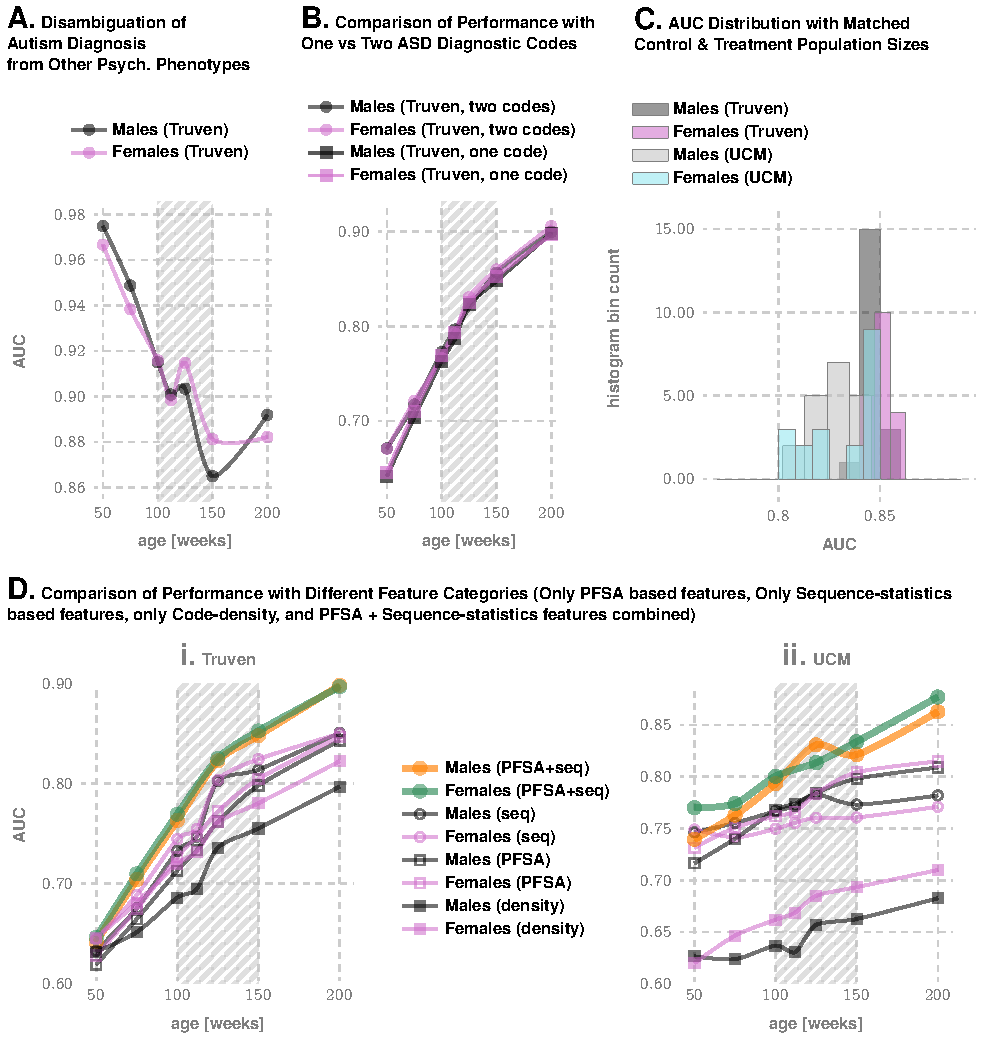
\includegraphics[width=0.95\textwidth]{Figures/External/sanitycheck}
  \fi 
  
 \captionN{\textbf{Evaluations of Feature Subsets, Class Imbalance, Code Density, Coding Uncertainty, \& Disambiguation from Other Psychiatric  Phenotypes.} Panel A illustrates that the pipeline performance where the control group is restricted to children to have at least one psychiatric phenotype other than ASD. It is clear that we have very good discrimination between ASD and non-ASD phenotypes. Panel B illustrates the situation where we restrict the treatment cohort to children to have at least $2$ AD diagnostic codes, to see whether the pipeline performance is markedly different in  populations where the coding errors/uncertainty is smaller. We see that such restrictions have no appreciable effect on  pipeline performance. Panel C illustrates the AUC distributions obtained by using sampled control cohorts that are of the same size as the treatment cohort, to evaluate the effect of class imbalance. Again we see that such restrictions do  not appreciably change performance. Panel D explores the performance changes when we use a restricted set of features, or simply use code density as the sole feature. We conclude that the combined feature set used in our optimized pipeline is superior to using the subsets individually. Code density is the least performant feature, and is not stable across databases. }\label{EXT-figcompsi}
\end{figure*} 
\else
\refstepcounter{figure}\label{EXT-figcompsi}
\fi
%###########################################################
%###########################################################

% ###########################################################
% ###########################################################
\ifFIGS
\begin{figure*}[!ht]
  \tikzexternalenable
    \tikzsetnextfilename{comorbidB}
  \vspace{-5pt}

\def\DATA{../../data_latest}
\iftikzX


\pgfplotsset{
    discard if/.style 2 args={
        x filter/.code={
            \edef\tempa{\thisrow{#1}}
            \edef\tempb{#2}
            \ifx\tempa\tempb
                \def\pgfmathresult{inf}
            \fi
        }
    },
    discard if not/.style 2 args={
        x filter/.code={
            \edef\tempa{\thisrow{#1}}
            \edef\tempb{#2}
            \ifx\tempa\tempb
            \else
                \def\pgfmathresult{inf}
            \fi
        }
    }
  }

  \begin{tikzpicture}[font=\bf\sffamily\fontsize{8}{10}\selectfont]
  \def\TEXTCOL{gray}
  \tikzset{
    hatch distance/.store in=\hatchdistance,
    hatch distance=20pt,
    hatch thickness/.store in=\hatchthickness,
    hatch thickness=2pt
  }


\pgfplotsset{
    accommodate labels/.code 2 args={
        \newlength{\myl}
        \pgfplotstableread{#1}\data
        \def\largestlength{0}
        \pgfplotstableforeachcolumnelement{#2}\of\data\as\cell{
            \settowidth{\myl}{\pgfinterruptpicture\cell\endpgfinterruptpicture}
            \pgfmathsetmacro\largestlength{max(\the\myl,\largestlength)}
        }
        \pgfplotsset{
            enlarge x limits={
                upper,              value=1/(1-(\largestlength+4pt)/\pgfkeysvalueof{/pgfplots/width})-1
            }
        }
    }
}

\def\COLDR{white}
\definecolor{alizarin}{rgb}{0.82, 0.1, 0.26}
\definecolor{amber}{rgb}{1.0, 0.75, 0.0}
\definecolor{amethyst}{rgb}{0.6, 0.4, 0.8}
\definecolor{apricot}{rgb}{0.98, 0.81, 0.69}
\definecolor{atomictangerine}{rgb}{1.0, 0.6, 0.4}
\definecolor{awesome}{rgb}{1.0, 0.13, 0.32}
\definecolor{azurec}{rgb}{0.0, 0.5, 1.0}
\definecolor{ballblue}{rgb}{0.13, 0.67, 0.8}
\definecolor{bittersweet}{rgb}{1.0, 0.44, 0.37}
\definecolor{bluem}{rgb}{0.0, 0.5, 0.69}
\definecolor{brightturquoise}{rgb}{0.03, 0.91, 0.87}

\def\COLBA{Red2}
\def\COLBB{Red3}
\def\COLBI{Red4}
\def\COLBG{DarkOrange2}
\def\COLBC{lightgray}
\def\COLBD{ballblue}
\def\COLBE{MidnightBlue}
\def\COLBF{SeaGreen3}
\def\COLBH{DarkSlateGray}
\def\COLBJ{bittersweet}
\def\COLBK{Orchid3}
\def\COLBL{black}
  
  % \makeatletter
  % \pgfdeclarepatternformonly[\hatchdistance,\hatchthickness]{flexible hatch}
  % {\pgfqpoint{0pt}{0pt}}
  % {\pgfqpoint{\hatchdistance}{\hatchdistance}}
  % {\pgfpoint{\hatchdistance-1pt}{\hatchdistance-1pt}}%
  % {
  %   \pgfsetcolor{\tikz@pattern@color}
  %   \pgfsetlinewidth{\hatchthickness}
  %   \pgfpathmoveto{\pgfqpoint{0pt}{0pt}}
  %   \pgfpathlineto{\pgfqpoint{\hatchdistance}{\hatchdistance}}
  %   \pgfusepath{stroke}
  % }
  % \makeatother
  % \pgfdeclarepatternformonly{north east lines wide}%
  % {\pgfqpoint{-1pt}{-1pt}}%
  % {\pgfqpoint{10pt}{10pt}}%
  % {\pgfqpoint{9pt}{9pt}}%
  % {
  %   \pgfsetlinewidth{0.4pt}
  %   \pgfpathmoveto{\pgfqpoint{0pt}{0pt}}
  %   \pgfpathlineto{\pgfqpoint{9.1pt}{9.1pt}}
  %   \pgfusepath{stroke}
  % }


  \def\COMPA{\DATA/figfiles/age_3_logodds_patternImmun.csv}
  \def\COMPB{\DATA/figfiles/age_3_logodds_patternnfect.csv}
  \def\COMPC{\DATA/figfiles/age_3_logodds_patternRespira.csv}
  \def\COMPD{\DATA/figfiles/age_3_logodds_patternCirculatory.csv} 
  \def\COMPINT{\DATA/figfiles/age_3_logodds_INTpattern.csv} 
 \def\MTYP{MImmun}
  \def\FTYP{FImmun}

  
  \def\WDTX{2.250in}
  \def\HGTX{3.75in}
  \def\HGTXB{5.65in}
  \def\HGTXC{6.25in}
  \def\HGTXD{2.5in}
  \def\HGTXE{4.325in}
  \def\OPC{1}
  \def\BWIDTH{6pt}
  \def\BWIDTHB{6pt}
  \clip (.75in,0.165in) rectangle (7.5in,-9.75in);


  
    \node [anchor=north west,align=left] (A) at (0,0.0) {
        \begin{tikzpicture}[text=\TEXTCOL]
%
%   \def\basis{1}
%   \pgfplotsset
%   {
%     x coord trafo/.code={\pgfmathparse{symlog(#1,\basis)}\pgfmathresult},
%     x coord inv trafo/.code={\pgfmathparse{symexp(#1,\basis)}\pgfmathresult},
%     xticklabel style={/pgf/number format/.cd,int detect,precision=2},
% } 


          \begin{axis}[legend style={anchor=east,at={(0.5,1.05)},inner sep=3pt,draw=none,fill=white,fill opacity=.850,align=right,text opacity=1,font=\bf\sffamily\fontsize{8}{9}\selectfont},axis line style={lightgray, opacity=0, thin},%
        enlargelimits=false,
        anchor=north west,
        height=\HGTX,
        width=\WDTX,
        %ymax=35,
        % xbar,
        ytick=data,% crucial line for the xticklabels directive 
        xmin=-2,
        %accommodate labels={\DISX}{description},
        yticklabels from table={\COMPA}{code},
        yticklabel style
        ={font=\bf\sffamily\fontsize{7}{7}\selectfont,
          align=right,rotate=0, text width=1.1in,
          anchor=east, yshift=0in,xshift=-.0450in,text=\TEXTCOL},
        major tick length=0pt,,text opacity=1,
        %xticklabel style=
        %{font=\bf\sffamily\fontsize{7}{7}\selectfont,
        %  text=\TEXTCOL},
        %grid,
        grid style={lightgray, dashed,opacity=.7},
        axis on top=false, bar width=\BWIDTH,
        xlabel={log odds ratio of normalized prevalence},
        scaled x ticks=false,
        xlabel style={yshift=0.05in,text=\TEXTCOL,text opacity=1},
        ylabel style={xshift=-.25in,yshift=0.075in,text=\TEXTCOL,text opacity=1},
        enlarge y limits=.04,
         x tick label style={/pgf/number format/fixed,/pgf/number format/precision=2,/pgf/number format/fixed zerofill,
     /pgf/number format/1000 sep = %\thinspace % Optional if you want to replace comma as the 1000 separator 
   },
   nodes near coords,visualization depends on={value \thisrow{negval}\as\rawx},
    every node near coord/.append style={anchor=west,align=left, text width=2in,font=\sffamily\rm\fontsize{8}{8}\selectfont,text=darkgray,text opacity=1,
        shift={(axis direction cs:-\rawx,0)}},
   point meta=explicit symbolic,ylabel={},
   , %xtick ={-0.03,0,0.03},
  % xmax=0.03,xmin=-0.03,
        ] 

        \addplot[draw=none,fill=none,xbar,area legend,opacity=0,text opacity=\OPC] table [ 
        y expr=\coordindex,
        x=pn,meta=description
        ] {\COMPA};

        \addplot[draw=\MXCOL,fill=\MXCOL,xbar,area legend,opacity=\OPC,text opacity=1] table [ 
        y expr=\coordindex,
        x=pn, discard if not={typ}{\MTYP}
        ] {\COMPA};
        \addplot[draw=\FXCOL,fill=\FXCOL,xbar,area legend,opacity=\OPC,text opacity=1] table [ 
        y expr=\coordindex,
        x=pn, discard if not={typ}{\FTYP}
        ] {\COMPA};

        
        % \addlegendentry{Female}
      \end{axis}
    \end{tikzpicture}};

      \node [anchor=north west,align=left] (B) at ([xshift=-1.68in,yshift=-0.0in]A.north east) {
        \begin{tikzpicture}[text=\TEXTCOL]
%
%   \def\basis{1}
%   \pgfplotsset
%   {
%     x coord trafo/.code={\pgfmathparse{symlog(#1,\basis)}\pgfmathresult},
%     x coord inv trafo/.code={\pgfmathparse{symexp(#1,\basis)}\pgfmathresult},
%     xticklabel style={/pgf/number format/.cd,int detect,precision=2},
% }


          \begin{axis}[legend style={anchor=east,at={(0.5,1.05)},inner sep=3pt,draw=none,fill=white,fill opacity=.85,align=right,text opacity=1,font=\bf\sffamily\fontsize{8}{9}\selectfont},axis line style={lightgray, opacity=0, thin},%
        enlargelimits=false,
        anchor=north west,
        height=\HGTXB,
        width=\WDTX,
        % xbar,
        ytick=data,% crucial line for the xticklabels directive 
        %xmin=0,
        %accommodate labels={\DISX}{description},
        yticklabels from table={\COMPB}{code},
        yticklabel style
        ={font=\bf\sffamily\fontsize{7}{7}\selectfont,
          align=right,rotate=0, text width=1.1in,
          anchor=east, yshift=0in,xshift=-.0450in,text=\TEXTCOL},
        major tick length=0pt,,text opacity=1,
        %xticklabel style=
        %{font=\bf\sffamily\fontsize{7}{7}\selectfont,
        %  text=\TEXTCOL},
        %grid
        grid style={lightgray, dashed,opacity=.7},
        axis on top=false, bar width=\BWIDTHB,
        xlabel={log odds ratio of normalized prevalence},
        scaled x ticks=false,
        xlabel style={yshift=0.05in,text=\TEXTCOL,text opacity=1},
        ylabel style={xshift=-2.25in,yshift=0.1in,text=\TEXTCOL,text opacity=1},
        enlarge y limits=.03,
         x tick label style={/pgf/number format/fixed,/pgf/number format/precision=2,/pgf/number format/fixed zerofill,
     /pgf/number format/1000 sep = %\thinspace % Optional if you want to replace comma as the 1000 separator 
   },
   nodes near coords,
       ,visualization depends on={value \thisrow{negval}\as\rawx},
    every node near coord/.append style={anchor=west,align=left, text width=2in,font=\sffamily\rm\fontsize{8}{8}\selectfont,text=darkgray,text opacity=1,
        shift={(axis direction cs:-\rawx,0)}},
   point meta=explicit symbolic,ylabel={ICD9 codes},
   , %xtick ={-0.03,0,0.03},
  % xmax=0.03,xmin=-0.03,
        ] 

        \addplot[draw=none,fill=none,xbar,area legend,opacity=0,text opacity=\OPC] table [ 
        y expr=\coordindex,
        x=pn, meta=description
        ] {\COMPB};

         
        \addplot[draw=\MXCOL,fill=\MXCOL,xbar,area legend,opacity=\OPC,text opacity=1] table [ 
        y expr=\coordindex,
        x=pn, discard if not={typ}{Mnfect}
        ] {\COMPB};

        
        \addplot[draw=\FXCOL,fill=\FXCOL,xbar,area legend,opacity=\OPC,text opacity=1] table [ 
        y expr=\coordindex,
        x=pn, discard if not={typ}{Fnfect}
        ] {\COMPB};

        
       \addplot[draw=\MXCOL,fill=\MXCOL,xbar,area legend,,postaction={
         pattern=flexible hatch,
        hatch distance=5pt,
        hatch thickness=1pt,
        draw=none,
        pattern color=gray, %ultra thick,
     },opacity=\OPC,text opacity=1] table [ 
        y expr=\coordindex,
        x=pn, discard if not={typ}{Mnfectv}
        ] {\COMPB};

        
        \addplot[draw=\FXCOL,fill=\FXCOL,xbar,area legend,postaction={
         pattern=flexible hatch,
        hatch distance=5pt,
        hatch thickness=1pt,
        draw=none,
        pattern color=black,  %ultra thick,
     },opacity=\OPC,text opacity=1] table [ 
        y expr=\coordindex,
        x=pn, discard if not={typ}{Fnfectv}
        ] {\COMPB};


        
        % \addlegendentry{Female}
      \end{axis}
    \end{tikzpicture}};

      \node [anchor=north west,align=left] (C) at ([yshift=-.2in]A.south west) {
        \begin{tikzpicture}[text=\TEXTCOL]
%
  \def\basis{1}
 %  \pgfplotsset
%   {
%     x coord trafo/.code={\pgfmathparse{symlog(#1,\basis)}\pgfmathresult},
%     x coord inv trafo/.code={\pgfmathparse{symexp(#1,\basis)}\pgfmathresult},
%     xticklabel style={/pgf/number format/.cd,int detect,precision=2},
% }


          \begin{axis}[legend style={anchor=east,at={(0.5,1.05)},inner sep=3pt,draw=none,fill=white,fill opacity=.85,align=right,text opacity=1,font=\bf\sffamily\fontsize{8}{9}\selectfont},axis line style={lightgray, opacity=0, thin},%
        enlargelimits=false,
        anchor=north west,
        height=\HGTXC,
        width=\WDTX,
        % xbar,
        ytick=data,% crucial line for the xticklabels directive 
        %xmin=0,
        %accommodate labels={\DISX}{description},
        yticklabels from table={\COMPC}{code},
        yticklabel style
        ={font=\bf\sffamily\fontsize{7}{7}\selectfont,
          align=right,rotate=0, text width=1.1in,
          anchor=east, yshift=0in,xshift=-.0450in,text=\TEXTCOL,text opacity=1},
        major tick length=0pt,
        %xticklabel style=
        %{font=\bf\sffamily\fontsize{7}{7}\selectfont,
        %  text=\TEXTCOL},
        %grid,
        grid style={lightgray, dashed,opacity=.7},
        axis on top=false, bar width=\BWIDTHB,
        xlabel={log odds ratio of normalized prevalence},
        scaled x ticks=false,
        xlabel style={yshift=0.05in,text=\TEXTCOL,text opacity=1},
        ylabel style={xshift=-.25in,yshift=0.075in,text=\TEXTCOL,text opacity=1},
        enlarge y limits=.03,
         x tick label style={/pgf/number format/fixed,/pgf/number format/precision=2,/pgf/number format/fixed zerofill,
     /pgf/number format/1000 sep = %\thinspace % Optional if you want to replace comma as the 1000 separator 
   },
    ,visualization depends on={value \thisrow{negval}\as\rawx},
    nodes near coords,
    every node near coord/.append style={%
       anchor=west, text width=2in,
      font=\sffamily\rm\fontsize{8}{8}\selectfont,text=darkgray,text opacity=1,
     shift={(axis direction cs:-\rawx,0)}
     },
     point meta=explicit symbolic,
    ylabel={},
   , %xtick ={-0.03,0,0.03},
  % xmax=0.03,xmin=-0.03,
        ] 

        \addplot[draw=none,fill=none,xbar,area legend,opacity=0,text opacity=\OPC] table [ 
        y expr=\coordindex,
        x=pn,meta=description
        ] {\COMPC};

        \addplot[draw=\MXCOL,fill=\MXCOL,xbar, area legend,opacity=\OPC,text opacity=1] table [ 
        y expr=\coordindex,
        x=pn, discard if not={typ}{MRespira}
        ] {\COMPC};
        \addplot[draw=\FXCOL,fill=\FXCOL,xbar,area legend,opacity=\OPC,text opacity=1] table [ 
        y expr=\coordindex,
        x=pn, discard if not={typ}{FRespira}
        ] {\COMPC};

      \end{axis}
    \end{tikzpicture}};


%       \node [anchor=north west,align=left] (D) at ([yshift=-.3in]B.south west) {
%         \begin{tikzpicture}[text=\TEXTCOL]
% %
%   \def\basis{1}
%  %  \pgfplotsset
% %   {
% %     x coord trafo/.code={\pgfmathparse{symlog(#1,\basis)}\pgfmathresult},
% %     x coord inv trafo/.code={\pgfmathparse{symexp(#1,\basis)}\pgfmathresult},
% %     xticklabel style={/pgf/number format/.cd,int detect,precision=2},
% % }


%           \begin{axis}[legend style={anchor=east,at={(0.5,1.05)},inner sep=3pt,draw=none,fill=white,fill opacity=.85,align=right,text opacity=1,font=\bf\sffamily\fontsize{8}{9}\selectfont},axis line style={lightgray, opacity=0, thin},%
%         enlargelimits=false,
%         anchor=north west,
%         height=\HGTXD,
%         width=\WDTX,
%         % xbar,
%         ytick=data,% crucial line for the xticklabels directive 
%         %ymax=15,
%         %accommodate labels={\DISX}{description},
%         yticklabels from table={\COMPD}{code},
%         yticklabel style
%         ={font=\bf\sffamily\fontsize{7}{7}\selectfont,
%           align=right,rotate=0, text width=1.1in,
%           anchor=east, yshift=0in,xshift=-.0450in,text=\TEXTCOL,text opacity=1},
%         major tick length=0pt,
%         %xticklabel style=
%         %{font=\bf\sffamily\fontsize{7}{7}\selectfont,
%         %  text=\TEXTCOL},
%         %grid,
%         grid style={lightgray, dashed,opacity=.7},
%         axis on top=false, bar width=\BWIDTHB,
%         xlabel={log odds ratio of normalized prevalence},
%         scaled x ticks=false,
%         xlabel style={yshift=0.05in,text=\TEXTCOL,text opacity=1},
%         ylabel style={xshift=-.25in,yshift=0.075in,text=\TEXTCOL,text opacity=1},
%         enlarge y limits=.04,
%          x tick label style={/pgf/number format/fixed,/pgf/number format/precision=2,/pgf/number format/fixed zerofill,
%      /pgf/number format/1000 sep = %\thinspace % Optional if you want to replace comma as the 1000 separator 
%    },
%     ,visualization depends on={value \thisrow{negval}\as\rawx},
%     nodes near coords,
%     every node near coord/.append style={%
%        anchor=west, text width=2in,
%       font=\sffamily\rm\fontsize{8}{8}\selectfont,text=darkgray,text opacity=1,
%      shift={(axis direction cs:-\rawx,0)}
%      },
%      point meta=explicit symbolic,
%     ylabel={},
%    , %xtick ={-0.03,0,0.03},
%   % xmax=0.03,xmin=-0.03,
%         ] 

%         \addplot[draw=none,fill=none,xbar,area legend,opacity=0,text opacity=\OPC] table [ 
%         y expr=\coordindex,
%         x=pn,meta=description
%         ] {\COMPD};

%         \addplot[draw=\MXCOL,fill=\MXCOL,xbar,postaction={
%          pattern=flexible hatch,
%         hatch distance=5pt,
%         hatch thickness=1pt,
%         draw=none,
%         pattern color=gray, %ultra thick,
%      }, area legend,opacity=\OPC,text opacity=1] table [ 
%         y expr=\coordindex,
%         x=pn, discard if not={typ}{MCirculatory}
%         ] {\COMPD};
%         \addplot[draw=\FXCOL,fill=\FXCOL,xbar,area legend,opacity=\OPC,text opacity=1] table [ 
%         y expr=\coordindex,
%         x=pn, discard if not={typ}{FCirculatory}
%         ] {\COMPD};

%       \end{axis}
%     \end{tikzpicture}};


      \node [anchor=north west,align=left] (D) at ([yshift=-.225in]B.south west) {
        \begin{tikzpicture}[text=\TEXTCOL]
%
  \def\basis{1}
 %  \pgfplotsset
%   {
%     x coord trafo/.code={\pgfmathparse{symlog(#1,\basis)}\pgfmathresult},
%     x coord inv trafo/.code={\pgfmathparse{symexp(#1,\basis)}\pgfmathresult},
%     xticklabel style={/pgf/number format/.cd,int detect,precision=2},
% }
\def\COMPX{\COMPINT}

          \begin{axis}[legend style={anchor=east,at={(0.5,1.05)},inner sep=3pt,draw=none,fill=white,fill opacity=.85,align=right,text opacity=1,font=\bf\sffamily\fontsize{8}{9}\selectfont},axis line style={lightgray, opacity=0, thin},%
        enlargelimits=false,
        anchor=north west,
        height=\HGTXE,
        width=\WDTX,
        % xbar,
        ytick=data,% crucial line for the xticklabels directive 
        %ymax=20,
        %accommodate labels={\DISX}{description},
        yticklabels from table={\COMPX}{code},
        yticklabel style
        ={font=\bf\sffamily\fontsize{7}{7}\selectfont,
          align=right,rotate=0, text width=1.1in,
          anchor=east, yshift=0in,xshift=-.0450in,text=\TEXTCOL,text opacity=1},
        major tick length=0pt,
        %xticklabel style=
        %{font=\bf\sffamily\fontsize{7}{7}\selectfont,
        %  text=\TEXTCOL},
        %grid,
        grid style={lightgray, dashed,opacity=.7},
        axis on top=false, bar width=\BWIDTHB,
        xlabel={log odds ratio of normalized prevalence},
        scaled x ticks=false,
        xlabel style={yshift=0.05in,text=\TEXTCOL,text opacity=1},
        ylabel style={xshift=-.25in,yshift=0.075in,text=\TEXTCOL,text opacity=1},
        enlarge y limits=.04,
         x tick label style={/pgf/number format/fixed,/pgf/number format/precision=2,/pgf/number format/fixed zerofill,
     /pgf/number format/1000 sep = %\thinspace % Optional if you want to replace comma as the 1000 separator 
   },
    ,visualization depends on={value \thisrow{negval}\as\rawx},
    nodes near coords,
    every node near coord/.append style={%
       anchor=west, text width=2in,
      font=\sffamily\rm\fontsize{8}{8}\selectfont,text=darkgray,text opacity=1,
     shift={(axis direction cs:-\rawx,0)}
     },
     point meta=explicit symbolic,
    ylabel={},
   , %xtick ={-0.03,0,0.03},
  % xmax=0.03,xmin=-0.03,
        ] 

        \addplot[draw=none,fill=none,xbar,area legend,opacity=0,text opacity=\OPC] table [ 
        y expr=\coordindex,
        x=pn,meta=description
        ] {\COMPX};

        \addplot[draw=\MXCOL,fill=\MXCOL,xbar, area legend,opacity=\OPC,text opacity=1] table [ 
        y expr=\coordindex,
        x=pn, discard if not={typ}{M}
        ] {\COMPX};
        \addplot[draw=\FXCOL,fill=\FXCOL,xbar,area legend,opacity=\OPC,text opacity=1] table [ 
        y expr=\coordindex,
        x=pn, discard if not={typ}{F}
        ] {\COMPX};

      \end{axis}
    \end{tikzpicture}};


    \node[] (T) at ([xshift=-1.4in,yshift=1.25in]B.east) {
      \arrayrulecolor{white}
      \setlength\arrayrulewidth{2pt}
      \mnp{1in}{\fontsize{9}{8}\selectfont\color{\TEXTCOL}
        {\large \color{black} Gender}
        \vskip 1em
        \begin{tabular}{L{.1in}L{.50in}}  %0
          \tikz[baseline=-0.5ex]{\node[text height=.075in,text width=.1in,fill=\MXCOL,,label={[]0:Male}] {};} 
          \tikz[baseline=-0.5ex]{\node[text height=.075in,text width=.1in,fill=\FXCOL,,label={[]0:Female}] {};}\\\hline          \tikz[baseline=-0.5ex]{\node[text height=.075in,text width=.1in,fill=none,,postaction={
         pattern=flexible hatch,
        hatch distance=5pt,
        hatch thickness=1pt,
        draw=none,
        pattern color=gray, %ultra thick,
     },label={[align=left]0:Viral/Fungal\\Inf.}] {};} 
          \end{tabular}
        }
      };
  
 \node[anchor=south west,align=left] (LA) at ([xshift=1in,yshift=-0.10in]A.north west) {{\LARGE A.} Endocrine Nutritional  Metabolic  And Immunity Dis.
 };
  \node[anchor=north west,align=left] (LB) at ([xshift=1in,yshift=-0in]$(LA.north west)!(B.west)!(LA.north east)$) 
{{\LARGE C.} Infectious And Parasitic Diseases
};
 \node[anchor=south west,align=left] (LD) at ([xshift=0in,yshift=-.1in]$(LB.north west)!(D.north)!(LB.south west)$) 
{{\LARGE D.} Similar Dis. with Opposed Association};
  \node[anchor=south west,align=left] (LC) at ([xshift=0in,yshift=-.05in]$(LA.north west)!(C.north)!(LA.south west)$)
  {{\LARGE B.} Respiratory Disorders };
\end{tikzpicture}


\else
  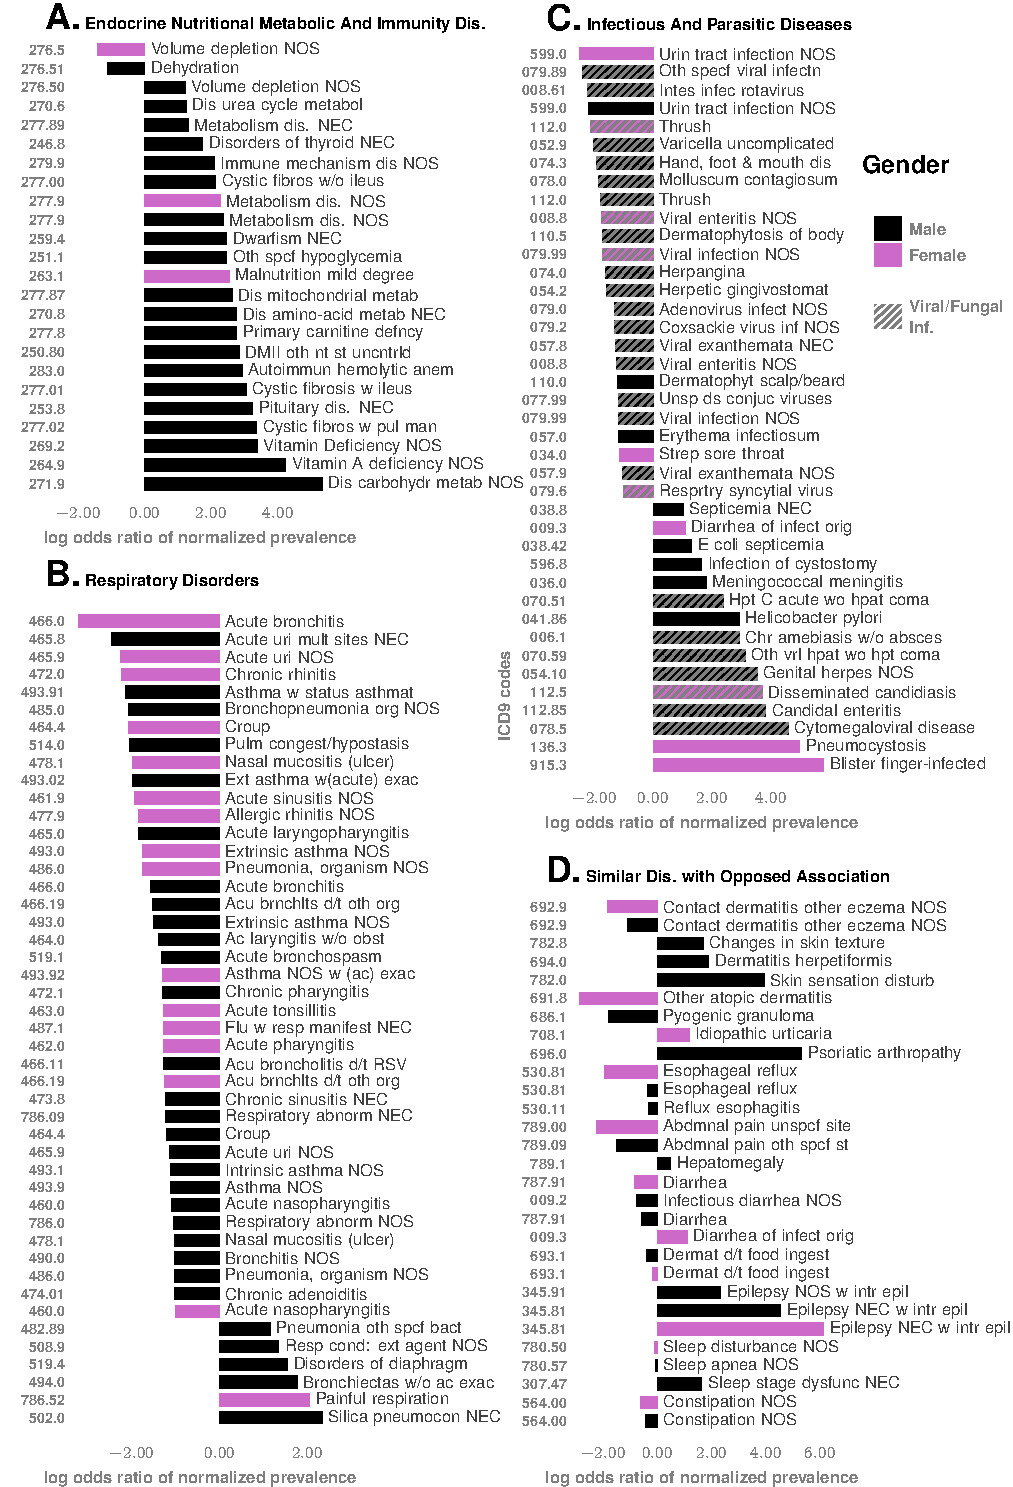
\includegraphics[width=0.8\textwidth]{Figures/External/comorbidB}
  \fi
  \vspace{-5pt}
  
  \captionN{\textbf{Details of Co-morbidity Patterns (at age $<3$ years)} for immunologic (panel A), respiratory (panel B), infections (panel C),  and disorders with similar pathobiology manifesting opposing association with autism (panel D).}\label{EXT-fig4}
    \vspace{-5pt}

\end{figure*}
\else
\refstepcounter{figure}\label{EXT-fig4}
\fi
%###########################################################
%###########################################################
% % ###########################################################
\ifFIGS
\begin{figure}[!ht]
  \tikzexternalenable
    \tikzsetnextfilename{comorbidC}

  \def\DATA{../../data_revision}

\iftikzX


\pgfplotsset{
    discard if/.style 2 args={
        x filter/.code={
            \edef\tempa{\thisrow{#1}}
            \edef\tempb{#2}
            \ifx\tempa\tempb
                \def\pgfmathresult{inf}
            \fi
        }
    },
    discard if not/.style 2 args={
        x filter/.code={
            \edef\tempa{\thisrow{#1}}
            \edef\tempb{#2}
            \ifx\tempa\tempb
            \else
                \def\pgfmathresult{inf}
            \fi
        }
    }
  }

  \begin{tikzpicture}[font=\bf\sffamily\fontsize{8}{10}\selectfont]
  \def\TEXTCOL{gray}
  \tikzset{
    hatch distance/.store in=\hatchdistance,
    hatch distance=20pt,
    hatch thickness/.store in=\hatchthickness,
    hatch thickness=2pt
  }


\pgfplotsset{
    accommodate labels/.code 2 args={
        \newlength{\myl}
        \pgfplotstableread{#1}\data
        \def\largestlength{0}
        \pgfplotstableforeachcolumnelement{#2}\of\data\as\cell{
            \settowidth{\myl}{\pgfinterruptpicture\cell\endpgfinterruptpicture}
            \pgfmathsetmacro\largestlength{max(\the\myl,\largestlength)}
        }
        \pgfplotsset{
            enlarge x limits={
                upper,              value=1/(1-(\largestlength+4pt)/\pgfkeysvalueof{/pgfplots/width})-1
            }
        }
    }
}

\def\COLDR{white}
\definecolor{alizarin}{rgb}{0.82, 0.1, 0.26}
\definecolor{amber}{rgb}{1.0, 0.75, 0.0}
\definecolor{amethyst}{rgb}{0.6, 0.4, 0.8}
\definecolor{apricot}{rgb}{0.98, 0.81, 0.69}
\definecolor{atomictangerine}{rgb}{1.0, 0.6, 0.4}
\definecolor{awesome}{rgb}{1.0, 0.13, 0.32}
\definecolor{azurec}{rgb}{0.0, 0.5, 1.0}
\definecolor{ballblue}{rgb}{0.13, 0.67, 0.8}
\definecolor{bittersweet}{rgb}{1.0, 0.44, 0.37}
\definecolor{bluem}{rgb}{0.0, 0.5, 0.69}
\definecolor{brightturquoise}{rgb}{0.03, 0.91, 0.87}

\def\COLBA{Red2}
\def\COLBB{Red3}
\def\COLBI{Red4}
\def\COLBG{DarkOrange2}
\def\COLBC{lightgray}
\def\COLBD{ballblue}
\def\COLBE{MidnightBlue}
\def\COLBF{SeaGreen3}
\def\COLBH{DarkSlateGray}
\def\COLBJ{bittersweet}
\def\COLBK{Orchid3}
\def\COLBL{black}
  
  \def\COMPA{\DATA/figfiles/Z2patternMental.csv}
  \def\COMPC{\DATA/figfiles/ZVplus.csv}
  \def\MTYP{MMental}
  \def\FTYP{FMental}
  \def\MTYPC{MV}
  \def\FTYPC{FV}


  
  \def\WDTX{2.20in}
  \def\HGTX{9.525in}
  \def\HGTXB{9.25in}
  \def\OPC{.9}
  \def\BWIDTH{10pt}
    \def\BWIDTHB{10pt}
  \def\BWIDTHC{7pt}  
  \clip (.85in,.3in) rectangle (7.5in,-9.25in);


  
    \node [anchor=north west,align=left] (A) at (0,0) {
        \begin{tikzpicture}[text=\TEXTCOL]
%
%   \def\basis{1}
%   \pgfplotsset
%   {
%     x coord trafo/.code={\pgfmathparse{symlog(#1,\basis)}\pgfmathresult},
%     x coord inv trafo/.code={\pgfmathparse{symexp(#1,\basis)}\pgfmathresult},
%     xticklabel style={/pgf/number format/.cd,int detect,precision=2},
% }


          \begin{axis}[yshift=1in,legend style={anchor=east,at={(0.5,2.75)},inner sep=3pt,draw=none,fill=white,fill opacity=.850,align=right,text opacity=1,font=\bf\sffamily\fontsize{8}{9}\selectfont},axis line style={lightgray, opacity=0, thin},%
        enlargelimits=false,
        anchor=north west,
        height=\HGTX,
        width=\WDTX,
        % xbar,
        ytick=data,% crucial line for the xticklabels directive 
        ymax=45, 
        %accommodate labels={\DISX}{description},
        yticklabels from table={\COMPA}{code},
        yticklabel style
        ={font=\bf\sffamily\fontsize{7}{7}\selectfont,
          align=right,rotate=0, text width=1.1in,
          anchor=east, yshift=0in,xshift=-.0450in,text=\TEXTCOL},
        major tick length=0pt,,text opacity=1,
        %xticklabel style=
        %{font=\bf\sffamily\fontsize{7}{7}\selectfont,
        %  text=\TEXTCOL},
        %grid,
        grid style={lightgray, dashed,opacity=.7},
        axis on top=false, bar width=\BWIDTH,
        xlabel={log odds ratio of normalized prevalence},
        scaled x ticks=false,
        xlabel style={yshift=0.3in,text=\TEXTCOL,text opacity=1},
        ylabel style={xshift=-.25in,yshift=0.075in,text=\TEXTCOL,text opacity=1},
        enlarge y limits=.05,
         x tick label style={/pgf/number format/fixed,/pgf/number format/precision=2,/pgf/number format/fixed zerofill,
           /pgf/number format/1000 sep = %\thinspace % Optional if you want to replace comma as the 1000 separator
          , yshift=0.21in,
   },
   nodes near coords,    ,visualization depends on={value \thisrow{negval}\as\rawx},
    every node near coord/.append style={anchor=west,align=left, text width=2in,font=\sffamily\rm\fontsize{8}{8}\selectfont,text=darkgray,text opacity=1,
        shift={(axis direction cs:-\rawx,0)}},
   point meta=explicit symbolic,ylabel={},
   , %xtick ={-0.03,0,0.03},
  % xmax=0.03,xmin=-0.03,
        ] 

        \addplot[draw=none,fill=none,xbar,area legend,opacity=0,text opacity=\OPC] table [ 
        y expr=\coordindex,
        x=pn,meta=description
        ] {\COMPA};

        \addplot[draw=\MXCOL,fill=\MXCOL,xbar,area legend,,postaction={
         pattern=flexible hatch,
        hatch distance=5pt,
        hatch thickness=1pt,
        draw=none,
        pattern color=gray, %ultra thick,
     },opacity=\OPC,text opacity=1] table [ 
        y expr=\coordindex,
        x=pn, discard if not={typ}{\MTYP}
        ] {\COMPA};
        \addplot[draw=\FXCOL,fill=\FXCOL,xbar,area legend,opacity=\OPC,text opacity=1] table [ 
        y expr=\coordindex,
        x=pn, discard if not={typ}{\FTYP}
        ] {\COMPA};

        
        % \addlegendentry{Female}
      \end{axis}
    \end{tikzpicture}};

      \node [anchor=north west,align=left] (B) at ([xshift=-1.55in,yshift=.01in]A.north east) {
        \begin{tikzpicture}[text=\TEXTCOL]
%
%   \def\basis{1}
%   \pgfplotsset
%   {
%     x coord trafo/.code={\pgfmathparse{symlog(#1,\basis)}\pgfmathresult},
%     x coord inv trafo/.code={\pgfmathparse{symexp(#1,\basis)}\pgfmathresult},
%     xticklabel style={/pgf/number format/.cd,int detect,precision=2},
% }


          \begin{axis}[legend style={anchor=east,at={(0.5,1.05)},inner sep=3pt,draw=none,fill=white,fill opacity=.85,align=right,text opacity=1,font=\bf\sffamily\fontsize{8}{9}\selectfont},axis line style={lightgray, opacity=0, thin},%
        enlargelimits=false,
        anchor=north west,
        height=\HGTXB,
        width=\WDTX,
        % xbar,
        % ymax=40,
        ymax=45,
        ytick=data,% crucial line for the xticklabels directive 
        %xmin=-2,
        %accommodate labels={\DISX}{description},
        yticklabels from table={\COMPC}{code},
        yticklabel style
        ={font=\bf\sffamily\fontsize{7}{7}\selectfont,
          align=right,rotate=0, text width=1.1in,
          anchor=east, yshift=0in,xshift=-.0450in,text=\TEXTCOL},
        major tick length=0pt,,text opacity=1,
        %xticklabel style=
        %{font=\bf\sffamily\fontsize{7}{7}\selectfont,
        %  text=\TEXTCOL},
        %grid
        grid style={lightgray, dashed,opacity=.7},
        axis on top=false, bar width=\BWIDTHB,
        xlabel={log odds ratio of normalized prevalence},
        scaled x ticks=false,
        xlabel style={yshift=0.03in,text=\TEXTCOL,text opacity=1},
        ylabel style={xshift=.25in,yshift=0.1in,text=\TEXTCOL,text opacity=1},
        enlarge y limits=.01,
         x tick label style={/pgf/number format/fixed,/pgf/number format/precision=2,/pgf/number format/fixed zerofill,
           /pgf/number format/1000 sep = %\thinspace % Optional if you want to replace comma as the 1000 separator
           , yshift=-0.05in
   },
   nodes near coords,    ,visualization depends on={value \thisrow{negval}\as\rawx},
    every node near coord/.append style={anchor=west,align=left, text width=2in,font=\sffamily\rm\fontsize{8}{8}\selectfont,text=darkgray,text opacity=1,
        shift={(axis direction cs:-\rawx,0)}},
   point meta=explicit symbolic,ylabel={ICD9 codes},
   , %xtick ={-0.03,0,0.03},
  % xmax=0.03,xmin=-0.03,
        ] 

        \addplot[draw=none,fill=none,xbar,area legend,opacity=0,text opacity=\OPC] table [ 
        y expr=\coordindex,
        x=pn, meta=description
        ] {\COMPC};

        \addplot[draw=\MXCOL,fill=\MXCOL,xbar,area legend,,postaction={
         pattern=flexible hatch,
        hatch distance=5pt,
        hatch thickness=1pt,
        draw=none,
        pattern color=gray, %ultra thick,
     },opacity=\OPC,text opacity=1] table [ 
        y expr=\coordindex,
        x=pn, discard if not={typ}{MV}
        ] {\COMPC};
        \addplot[draw=\FXCOL,fill=\FXCOL,xbar,area legend,opacity=\OPC,text opacity=1] table [ 
        y expr=\coordindex,
        x=pn, discard if not={typ}{FV}
        ] {\COMPC};

        
        % \addlegendentry{Female}
      \end{axis}
    \end{tikzpicture}};

%       \node [anchor=north west,align=left] (C) at ($(B.south west)!(A.north)!(B.north west)$) {
%         \begin{tikzpicture}[text=\TEXTCOL]
% %
% %   \def\basis{1}
% %   \pgfplotsset
% %   {
% %     x coord trafo/.code={\pgfmathparse{symlog(#1,\basis)}\pgfmathresult},
% %     x coord inv trafo/.code={\pgfmathparse{symexp(#1,\basis)}\pgfmathresult},
% %     xticklabel style={/pgf/number format/.cd,int detect,precision=2},
% % }


%           \begin{axis}[legend style={anchor=east,at={(0.5,1.05)},inner sep=3pt,draw=none,fill=white,fill opacity=.85,align=right,text opacity=1,font=\bf\sffamily\fontsize{8}{9}\selectfont},axis line style={lightgray, opacity=0, thin},%
%         enlargelimits=false,
%         anchor=north west,
%         height=\HGTXC,
%         width=\WDTX,
%         % xbar,
%         ytick=data,% crucial line for the xticklabels directive 
%         %xmin=0,
%         %accommodate labels={\DISX}{description},
%         yticklabels from table={\COMPC}{code},
%         yticklabel style
%         ={font=\bf\sffamily\fontsize{7}{7}\selectfont,
%           align=right,rotate=0, text width=1.1in,
%           anchor=east, yshift=0in,xshift=-.0450in,text=\TEXTCOL,text opacity=1},
%         major tick length=0pt,
%         %xticklabel style=
%         %{font=\bf\sffamily\fontsize{7}{7}\selectfont,
%         %  text=\TEXTCOL},
%         %grid,
%         grid style={lightgray, dashed,opacity=.7},
%         axis on top=false, bar width=\BWIDTHC,
%         xlabel={log odds ratio of normalized prevalence},
%         scaled x ticks=false,
%         xlabel style={yshift=0.05in,text=\TEXTCOL,text opacity=1},
%         ylabel style={xshift=-.25in,yshift=0.075in,text=\TEXTCOL,text opacity=1},
%         enlarge y limits=.03,
%          x tick label style={/pgf/number format/fixed,/pgf/number format/precision=2,/pgf/number format/fixed zerofill,
%      /pgf/number format/1000 sep = %\thinspace % Optional if you want to replace comma as the 1000 separator 
%    },
%    nodes near coords,    ,visualization depends on={value \thisrow{negval}\as\rawx},
%     every node near coord/.append style={anchor=west,align=left, text width=2in,font=\sffamily\rm\fontsize{8}{8}\selectfont,text=darkgray,text opacity=1,
%         shift={(axis direction cs:-\rawx,0)}},
%    point meta=explicit symbolic,ylabel={},
%    , %xtick ={-0.03,0,0.03},
%   % xmax=0.03,xmin=-0.03,
%         ] 

%         \addplot[draw=none,fill=none,xbar,area legend,opacity=0,text opacity=\OPC] table [ 
%         y expr=\coordindex,
%         x=pn,meta=description
%         ] {\COMPC};

%         \addplot[draw=\MXCOL,fill=\MXCOL,xbar,area legend,,postaction={
%          pattern=flexible hatch,
%         hatch distance=5pt,
%         hatch thickness=1pt,
%         draw=none,
%         pattern color=gray, %ultra thick,
%      },opacity=\OPC,text opacity=1] table [ 
%         y expr=\coordindex,
%         x=pn, discard if not={typ}{Merinatal}
%         ] {\COMPC};
%         \addplot[draw=\FXCOL,fill=\FXCOL,xbar,area legend,opacity=\OPC,text opacity=1] table [ 
%         y expr=\coordindex,
%         x=pn, discard if not={typ}{Ferinatal}
%         ] {\COMPC};

        
        % \addlegendentry{Female}
    %  \end{axis}
    %\end{tikzpicture}};
    \node[] (T) at ([xshift=-1.35in,yshift=2.5in]A.east) {
      \arrayrulecolor{white}
      \setlength\arrayrulewidth{2pt}
      \mnp{1in}{\fontsize{9}{8}\selectfont\color{\TEXTCOL}
        {\large \color{black} Gender}
        \vskip 1em
        \begin{tabular}{L{.1in}L{.5in}}
          \tikz[baseline=-0.5ex]{\node[text height=.075in,text width=.1in,fill=\MXCOL,,postaction={
         pattern=flexible hatch,
        hatch distance=5pt,
        hatch thickness=1pt,
        draw=none,
        pattern color=gray, %ultra thick,
     },label={[]0:Male}] {};} \\\hline  %0
          \tikz[baseline=-0.5ex]{\node[text height=.075in,text width=.1in,fill=\FXCOL,,label={[]0:Female}] {};} 
          \end{tabular}
        }
      };

  \node[anchor=south west,align=left] (LA) at ([xshift=1in,yshift=0in]A.north west) {{\LARGE A.} Mental Disorders };
  \node[anchor=south west,align=left] (LB) at ([xshift=3.5in,yshift=0in]$(LA.north west)!(A.north)!(LA.south west)$) {{\LARGE B.} Vaccinations \& Health Service Encounters};

 %  \node[anchor=south west,align=left] (LC) at ([xshift=3.5in,yshift=-4.5in]$(LA.north west)!(C.north)!(LA.south west)$) {{\LARGE C.} Digestive System Disorders
 % };
 
\end{tikzpicture}


\else
  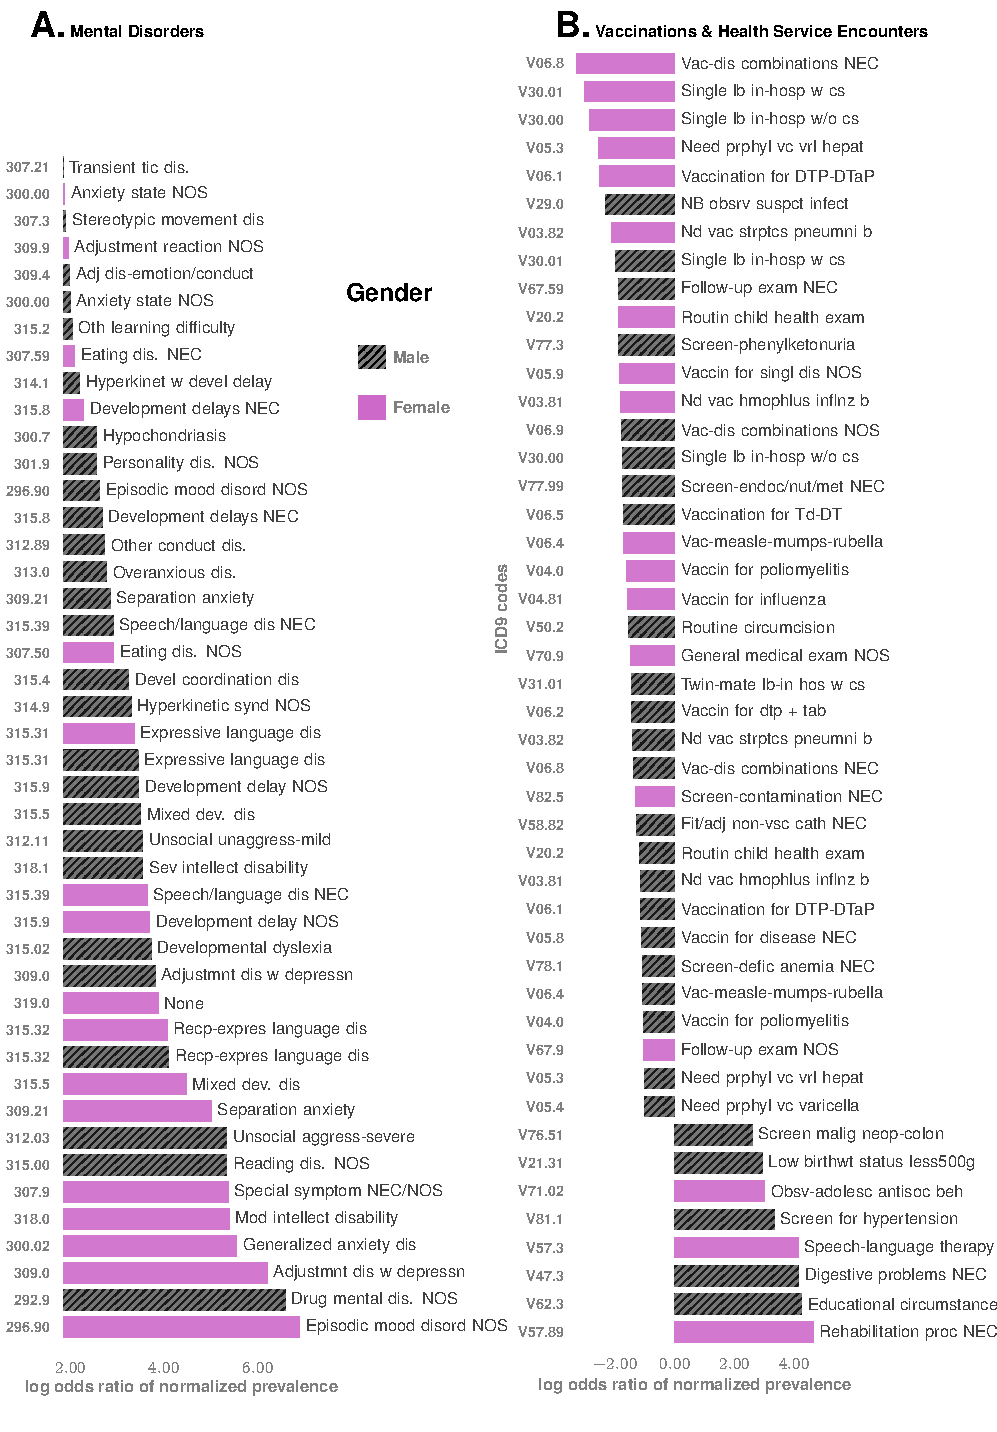
\includegraphics[width=0.9\textwidth]{Figures/External/comorbidC}
  \fi

  \vspace{-0pt}
  
  \captionN{\textbf{Co-morbidity Patterns}  for mental disorders, vaccinations and health-service encounters.}\label{EXT-figvv1}
\end{figure}%##########################################################
\else
\refstepcounter{figure}\label{EXT-figvv1}
\fi
% % % ###########################################################%
%###########################################################
%###############################################
%###########################################################
\ifFIGS
\begin{figure*}[!ht]
  \tikzexternalenable
    \tikzsetnextfilename{nopsych}
  \centering  
  \vspace{-10pt}
  
  \def\DATA{../../data_latest}
  \iftikzX
\begin{tikzpicture}[font=\bf\sffamily\fontsize{8}{10}\selectfont]
\def\TEXTCOL{gray}
    % \tikzset{
    %     hatch distance/.store in=\hatchdistance,
    %     hatch distance=20pt,
    %     hatch thickness/.store in=\hatchthickness,
    %     hatch thickness=2pt
    % }

% defining the new dimensions and parameters
\newlength{\hatchspread}
\newlength{\hatchthickness}
\newlength{\hatchshift}
\newcommand{\hatchcolor}{}
% declaring the keys in tikz
\makeatletter
\tikzset{hatchspread/.code={\setlength{\hatchspread}{#1}},
         hatchthickness/.code={\setlength{\hatchthickness}{#1}},
         hatchshift/.code={\setlength{\hatchshift}{#1}},% must be >= 0
         hatchcolor/.code={\renewcommand{\hatchcolor}{#1}}}
% setting the default values
\tikzset{hatchspread=3pt,
         hatchthickness=0.4pt,
         hatchshift=0pt,% must be >= 0
         hatchcolor=black}
% declaring the pattern
\pgfdeclarepatternformonly[\hatchspread,\hatchthickness,\hatchshift,\hatchcolor]% variables
   {custom north west lines}% name
   {\pgfqpoint{\dimexpr-2\hatchthickness}{\dimexpr-2\hatchthickness}}% lower left corner
   {\pgfqpoint{\dimexpr\hatchspread+2\hatchthickness}{\dimexpr\hatchspread+2\hatchthickness}}% upper right corner
   {\pgfqpoint{\dimexpr\hatchspread}{\dimexpr\hatchspread}}% tile size
   {% shape description
    \pgfsetlinewidth{\hatchthickness}
    \pgfpathmoveto{\pgfqpoint{0pt}{\dimexpr\hatchspread+\hatchshift}}
    \pgfpathlineto{\pgfqpoint{\dimexpr\hatchspread+0.15pt+\hatchshift}{-0.15pt}}
    \ifdim \hatchshift > 0pt
      \pgfpathmoveto{\pgfqpoint{0pt}{\hatchshift}}
      \pgfpathlineto{\pgfqpoint{\dimexpr0.15pt+\hatchshift}{-0.15pt}}
    \fi
    \pgfsetstrokecolor{\hatchcolor}
%    \pgfsetdash{{1pt}{1pt}}{0pt}% dashing cannot work correctly in all situation this way
    \pgfusepath{stroke}
   }
 \makeatother


%     \makeatletter
%     \pgfdeclarepatternformonly[\hatchdistance,\hatchthickness]{flexible hatch}
%     {\pgfqpoint{0pt}{0pt}}
%     {\pgfqpoint{\hatchdistance}{\hatchdistance}}
%     {\pgfpoint{\hatchdistance-1pt}{\hatchdistance-1pt}}%
%     {
%         \pgfsetcolor{\tikz@pattern@color}
%         \pgfsetlinewidth{\hatchthickness}
%         \pgfpathmoveto{\pgfqpoint{0pt}{0pt}}
%         \pgfpathlineto{\pgfqpoint{\hatchdistance}{\hatchdistance}}
%         \pgfusepath{stroke}
%     }
%     \makeatother
% \pgfdeclarepatternformonly{north east lines wide}%
%    {\pgfqpoint{-1pt}{-1pt}}%
%    {\pgfqpoint{10pt}{10pt}}%
%    {\pgfqpoint{9pt}{9pt}}%
%    {
%      \pgfsetlinewidth{0.4pt}
%      \pgfpathmoveto{\pgfqpoint{0pt}{0pt}}
%      \pgfpathlineto{\pgfqpoint{9.1pt}{9.1pt}}
%      \pgfusepath{stroke}
%     }


  \def\WDT{4.75in} 
  \def\WDTA{2in}    

  
  \def\datafile{\DATA/figfiles/AUC.csv}
  \def\datafileimp{\DATA/figfiles/AUC_imputed.csv}
 % \def\CHLM{Figures/augmented_M_fips_auc_rainbow}
 % \def\CHLF{Figures/augmented_F_fips_auc_rainbow}

  \def\CHLM{\DATA/figfiles/augmented_M_fips_auc_rainbow0}
  \def\CHLF{\DATA/figfiles/augmented_F_fips_auc_rainbow0}
  % \def\CHLM{Figures/augmented_M_fips_auc_Spectral_r0}
  % \def\CHLF{Figures/augmented_F_fips_auc_Spectral_r0}
  % \def\CHLM{Figures/augmented_M_fips_auc_Purples0}
  % \def\CHLF{Figures/augmented_F_fips_auc_Purples0}

  \def\ROCF{\DATA/figfiles/ROC_F_s.csv}
  \def\ROCM{\DATA/figfiles/ROC_M_s.csv}
  \def\IMP{\DATA/figfiles/importance20.csv}
 % \def\IMP{\DATA/figfiles/importance15.csv}
  \def\INTF{Figures/intf.dat}

  \def\HGT{1.30in}
  \def\WDT{6in}
  \def\WDTC{4in}
  \def\WDTR{1.9in}
  \def\WDTH{1.7in}
  
  \node[] (A) at (0,0) {};
  \node [anchor=north] (M) at (A.south) {\includegraphics[width=\WDTC]{\CHLM}};
  \node [anchor=north] (F) at ([yshift=-0.8in]M.south) {\includegraphics[width=\WDTC]{\CHLF}};
  
  % \begin{axis}[legend cell align=left,text=\TEXTCOL,
  %   legend style={text=black,anchor=east,at={(0.32,0.4)},inner sep=3pt,draw=none,fill=lightgray!10,fill opacity=.35,align=right,text opacity=1},
  %   name=E,
  %   at=(F.south west),
  %   xshift=0.6in,
  %   yshift=-0.7in,
  %   anchor=north west,
  %   width=\WDT,
  %   height=\HGT,
  %   ybar,
  %   bar width=4pt,
  %   xmin=.6,
  %   xmax=1,
  %   scale only axis=true, 
  %   axis on top=false,
  %   % axis background/.style={
  %   % shade,top color=transparent!15,bottom color=transparent!10},
  %   axis line style={lightgray!2, thin},
  %   grid,
  %   grid style={dashed,opacity=.95,thin,black!10},
  %   % xticklabel style={xshift=0.05in,yshift=-.05in},
  %   % xlabel style={xshift=-.075in,yshift=.05in,text=black},
  %   ylabel style={align=center,,text=black,anchor=center,
  %     yshift=-.1in,xshift=-.1in,font=\bf\sffamily\fontsize{7}{8}\selectfont,text=\TEXTCOL},
  %   % tickpos=left,
  %   ytick align=outside,
  %   xtick align=outside,
  %   major tick length=0pt,
  %   scaled y ticks = false,
  %   y tick label style={/pgf/number format/fixed,
  %     /pgf/number format/1000 sep = \thinspace % Optional if you want to replace comma as the 1000 separator 
  %   },
  %   ylabel={probability},
  %   ytick={0,0.02,0.04,0.06,0.08},
  %   ]
  %   \addplot [draw=none, thin, fill=\FXCOL,,fill opacity=1,, area legend]table [col sep=comma,x=AUC,y=F, area legend] {\datafileimp};
  %   \addlegendentry{AUC (Female)};
  %   \addplot [draw=none, thin, fill=\MXCOL,fill opacity=1, area legend] table [col sep=comma,x=AUC,y=M, area legend] {\datafileimp};
  %   \addlegendentry{AUC (Male)};
  %   % \draw[very thick,Red2] (axis cs:0.677,\pgfkeysvalueof{/pgfplots/ymin}) -- (axis cs:0.677,\pgfkeysvalueof{/pgfplots/ymax}) node [midway,right,fill=white,fill opacity=.9,text opacity=1,inner sep=2pt,pos=0.2,font=\sffamily\fontsize{6}{6}\selectfont] {0.677};
  %   % \draw[very thick,Red2] (axis cs:0.73,\pgfkeysvalueof{/pgfplots/ymin}) -- (axis cs:0.73,\pgfkeysvalueof{/pgfplots/ymax}) node [midway,right,fill=white,fill opacity=.9,text opacity=1,inner sep=2pt,pos=0.2,font=\sffamily\fontsize{6}{6}\selectfont] {0.73};
  % \end{axis}
  
  \node [anchor=north east, align=left,align=left] (B) at ([xshift=-0.35in,yshift=0.1in]M.north west) {
    \begin{tikzpicture}[anchor=center]
    \begin{axis}[legend cell align=left,text=\TEXTCOL, legend style={text=black,anchor=east,at={(1,0.12)},inner sep=1pt,draw=none,fill=gray!19,fill opacity=.85,align=right,text opacity=1,font=\bf\sffamily\fontsize{7}{8}\selectfont},
    name=K,
    clip=false,
    %at=(CC.center),
    xshift=-0in,
    yshift=-.25in,
    anchor=center,
    width=\WDTR,
    height=\WDTH,
    scale only axis=true,
    enlargelimits=false,
    axis on top=false,
     axis background/.style={
     shade,top color=transparent!0,bottom color=transparent!15},
    axis line style={black!2, very thick},
    grid,
    grid style={opacity=.9,thin,black!20},
    % xticklabel style={xshift=0.05in,yshift=-.05in},
    xlabel style={yshift=.05in,text=\TEXTCOL},
    ylabel style={align=center,,text=\TEXTCOL,anchor=center,
      yshift=-.175in},
    % tickpos=left,
    ytick align=outside,
    xtick align=outside,
    major tick length=0pt,
    scaled y ticks = false,
    y tick label style={/pgf/number format/fixed,
      /pgf/number format/1000 sep = \thinspace % Optional if you want to replace comma as the 1000 separator 
    },
    ylabel={TPR},xlabel={FPR},
    xmin=-0.05,
    ymax=1.02,
    extra x ticks={1},extra x tick labels={1}]
%
    \def\LCOL{Red1}
        \addplot [name path=a,smooth,draw=\FXCOL, ultra thick, fill=none,, pattern color=\FXCOL,pattern=custom north west lines,hatchspread=6pt,hatchthickness=3pt,fill opacity=.35,hatchcolor=Orchid3!60]table [col sep=comma,x=fpr ,y=tpr] {\ROCF};
          \addlegendentry{Female (AUC 81.6\%)}
  \addplot [smooth,draw=\MXCOL, ultra thick, fill=none,fill opacity=.5,]table [col sep=comma,x=fpr ,y=tpr] {\ROCM};
    \addlegendentry{Male (AUC 84.4\%)} 


\draw[name path=b,smooth,draw=\LCOL,,,very thick] (axis cs:0.05,0) -- (axis cs:0.05,\pgfkeysvalueof{/pgfplots/ymax})
      %\addplot [name path=b,smooth,draw=\LCOL,,,very thick]table [col sep=comma,x=fpr ,y=tpr] {\INTF} 
node [fill=white,midway,sloped,above,right,pos=.725,yshift=-.165in,text=\LCOL,align=center,font=\bf\sffamily\fontsize{7}{8}\selectfont] {specificity \\95.0\%};
      %\draw[Red1,name path=b,] (axis cs:0.05,0) -- (axis cs:0.05,1);
      \fill [name intersections={of=a and b},Red1] (intersection-1) circle (2pt)coordinate (c) ;


      \draw [\LCOL,very thick] (c) -- ($(axis cs:\pgfkeysvalueof{/pgfplots/xmin},0)!(c)!(axis cs:\pgfkeysvalueof{/pgfplots/xmin},1)$) ;
      \draw [\LCOL,very thick] (c) -- ($(axis cs:1,0)!(c)!(axis cs:1,1)$)node [font=\bf\sffamily\fontsize{7}{8}\selectfont,fill=lightgray!50,midway,below,pos=.7,yshift=-.1in,xshift=-.1in,text=\LCOL] {sensitivity: 51.8\%\\PPV (Male): 15.8\%\\PPV (Female): 18.8\%};
      % \draw [black,name path=d] (axis cs:0,0.38) -- (axis cs:1,.38)node [midway,below,pos=.65] {M-CHAT/F 38.8\%};
      % \fill [name intersections={of=d and b},black] (intersection-1) circle (2pt)coordinate (dd) ;
      %\draw[ultra thin,dashed,black] (c) -- (axis cs:1,.5175);
    \end{axis}
    \end{tikzpicture} 
  };
%
  \node [anchor=north east,align=left] (R) at ([xshift=-1.55in,yshift=1in]F.north west) {

\begin{axis}[legend cell align=left,legend style={anchor=east,at={(.9,0.1)},inner sep=3pt,draw=none,fill=white,fill opacity=.85,align=right,text opacity=1,font=\bf\sffamily\fontsize{8}{9}\selectfont},axis line style={lightgray, opacity=0, thin},%
enlargelimits=true,
%grid,
xshift=.1in,
anchor=north west,
  height=4in,
width=2.15in,
    xbar, 
    ytick=data,% crucial line for the xticklabels directive 
    ymin=0, 
    yticklabels from table={\IMP}{feature},
        yticklabel style={font=\bf\sffamily\fontsize{7}{7}\selectfont,align=right,rotate=0, text width=1.1in, anchor=east, yshift=0in,xshift=-.045in,text=\TEXTCOL},
major tick length=0pt,
xticklabel style={font=\bf\sffamily\fontsize{7}{7}\selectfont,text=\TEXTCOL},
grid,
grid style={lightgray, opacity=.7},
axis on top=false, bar width=4.2pt,xlabel={importance},xlabel style={yshift=0.05in,text=\TEXTCOL},
enlarge y limits=0.03,
] 

\addplot[opacity=1,fill=\MXCOL, area legend] table [ 
    y expr=\coordindex,
    x=M
] {\IMP};   
\addlegendentry{Male}
\addplot[opacity=1,fill=\FXCOL, area legend] table [ 
    y expr=\coordindex,
    x=F
] {\IMP};   
\addlegendentry{Female}

\end{axis} 

  };

  \node[anchor=south west,align=left] (LA) at ([xshift=.2in,yshift=0in]M.north west) {{\LARGE C.} AUC Spatial Variation (Males)   };
  \node[anchor=south west,align=left] (LB) at ([xshift=.2in,yshift=0in]F.north west) {{\LARGE D.} AUC Spatial Variation (Females)   };
  %\node[anchor=south west,align=left] (LC) at ([xshift=0in,yshift=.1in]$(LA.west)!(E.north west)!(LB.west)$) {{\LARGE C.} AUC Distribution over US Counties};
  \node[anchor=north west,align=left] (LD) at ([xshift=-0in,yshift=0in]$(B.west)!(LA.north)!(B.north west)$) {{\LARGE A.} ROC Curves at $150$ weeks  };

  \node[anchor=south west,align=left] (LR) at ([xshift=-0in,yshift=0.05in]$(LD.north west)!(R.north)!(LD.south west)$) {{\LARGE B.} Top 20  Phenotype-specific Features };

\end{tikzpicture}

\else
  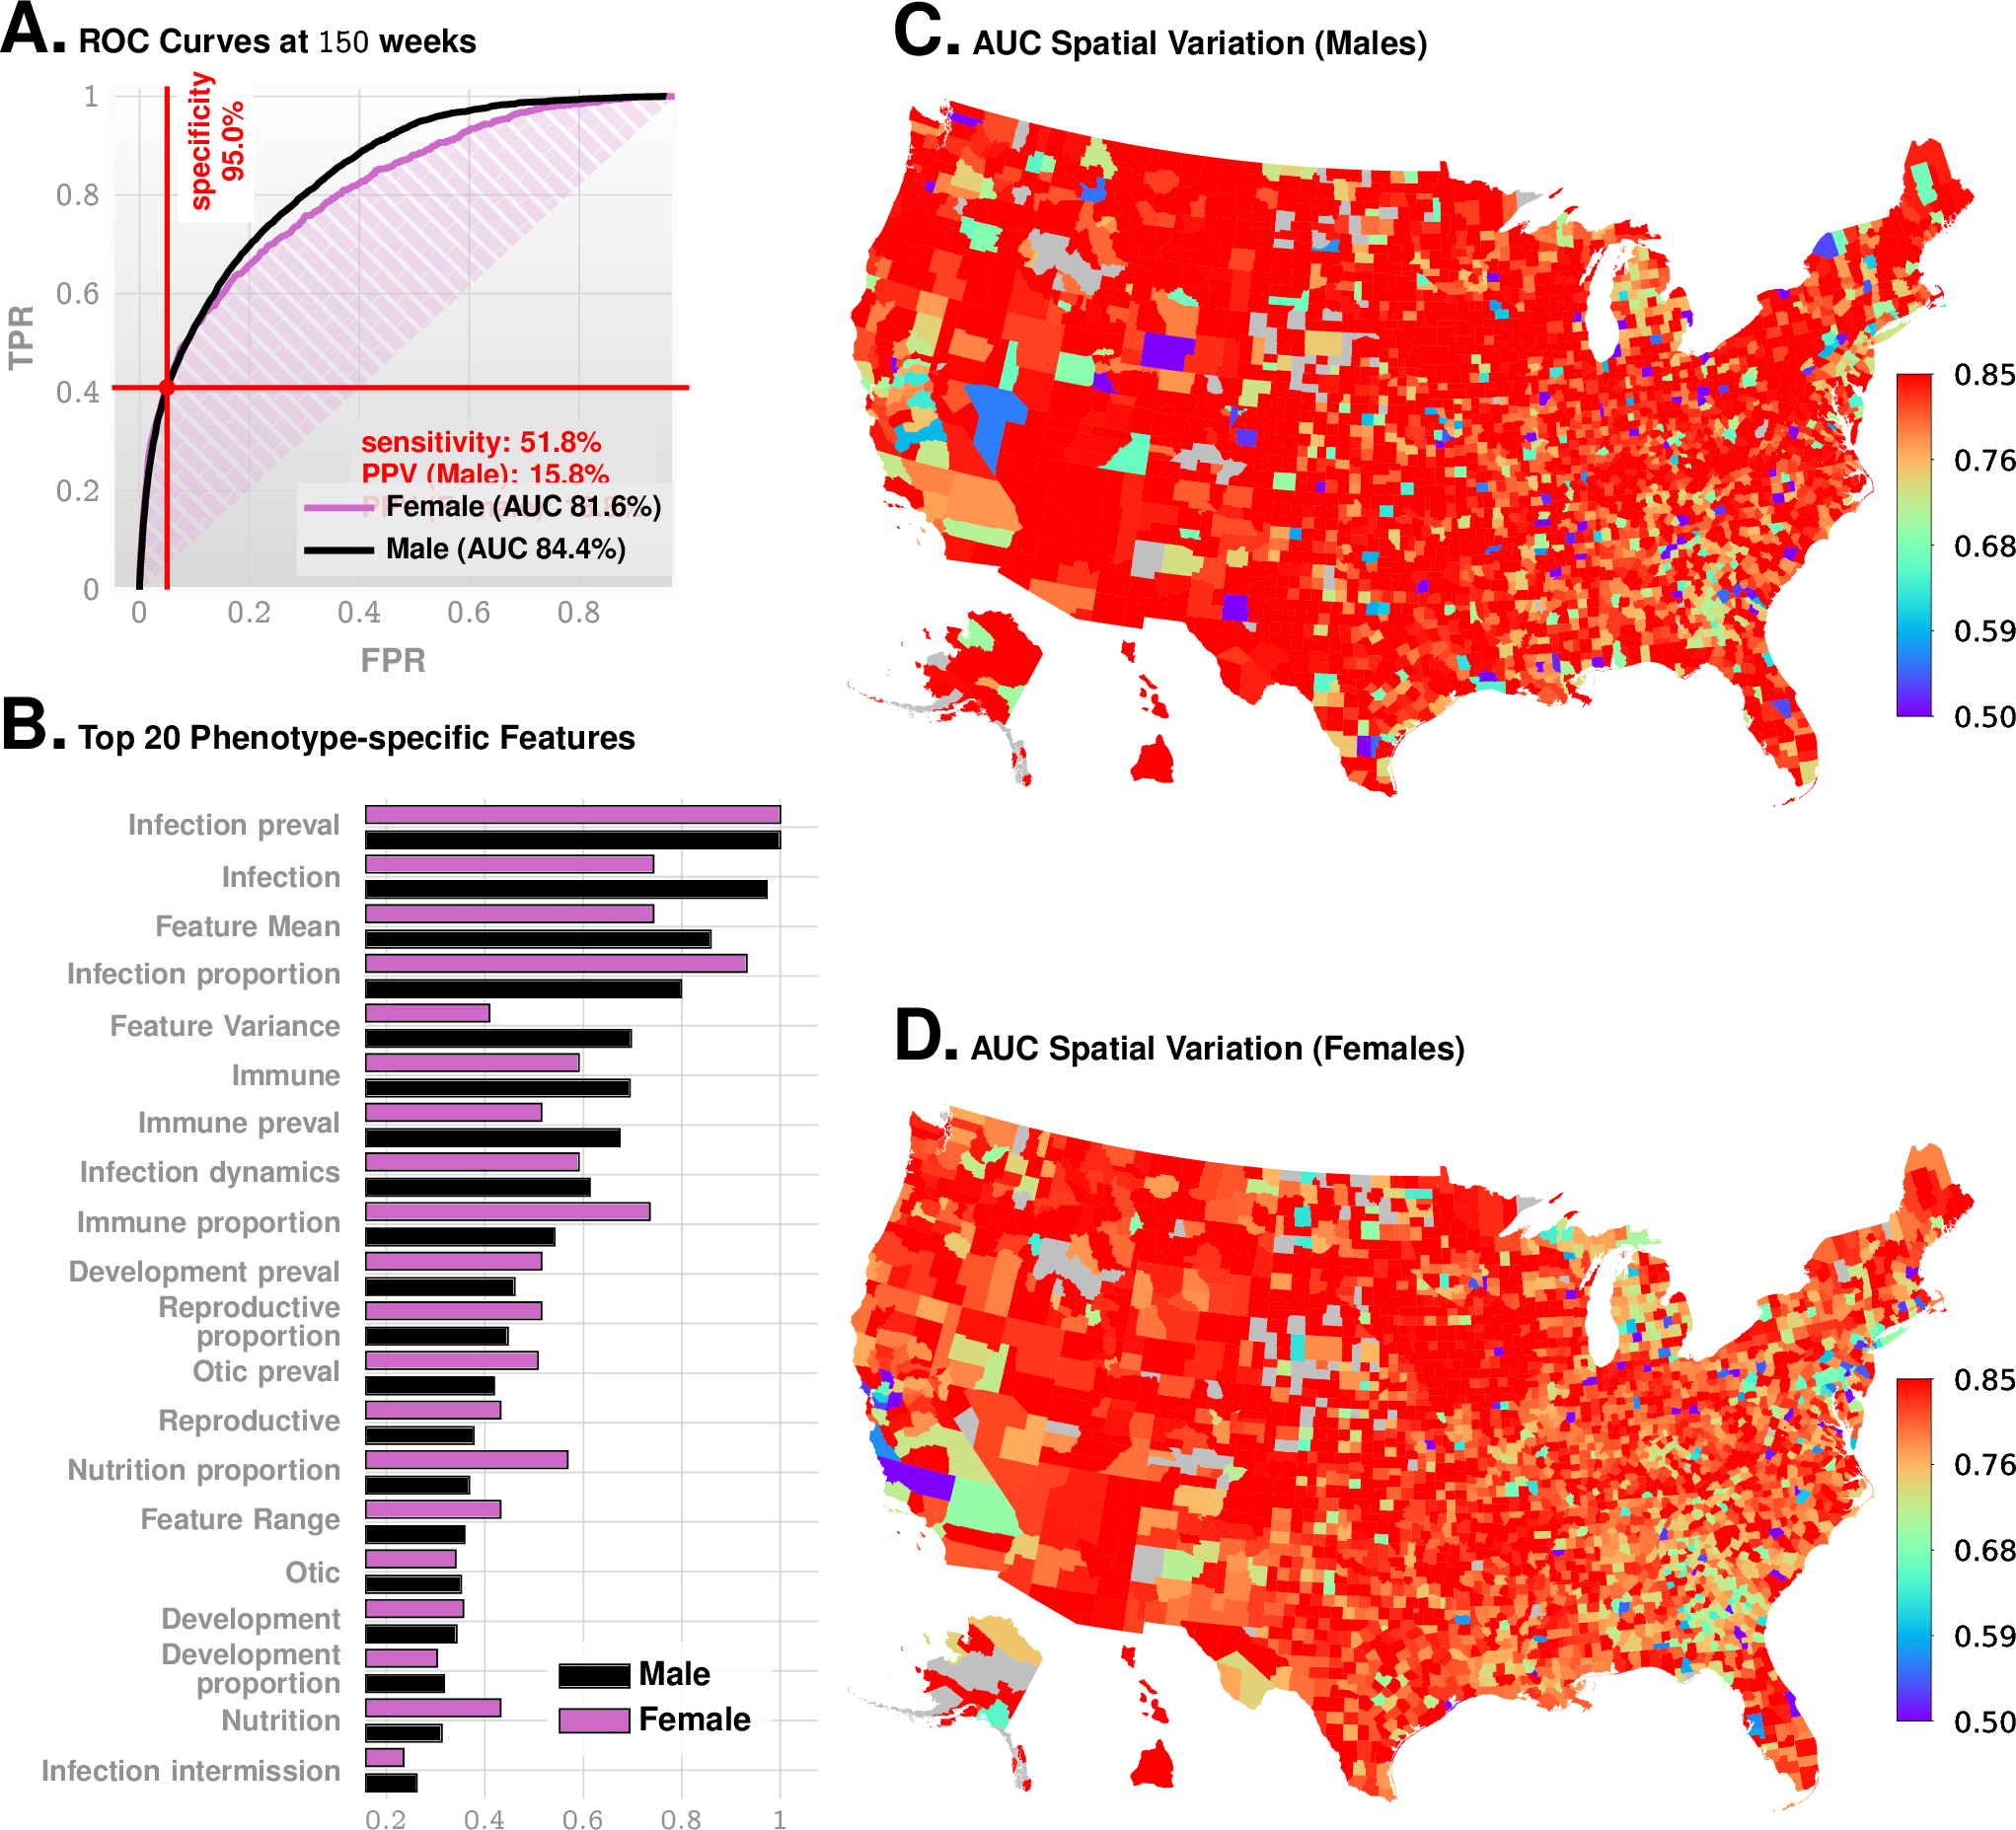
\includegraphics[width=0.95\textwidth]{Figures/External/nopsych}
  \fi 
     \vspace{-5pt}

     \captionN{Predictive Performance without psychiatric codes (ICD9 290 - 319)  and codes for health status and services (ICD9 V0-V91)  included. As shown, the performance is comparable at 150 weeks, with the AUC for females marginally lower (compare with Fig.~\ref{main-fig1} in the main text). The feature importances also are similar, with infectious diseases inferred to have the most importance (or weight) in the pipeline, which is also the case once we add psychiatric phenotypes, and codes for health services in our analysis. As shown in  SI-Fig.~\ref{EXT-figvv1}A, the psychiatric codes all increase risk, and the vaccination codes (See  SI-Fig.~\ref{EXT-figvv1}B) all decrease risk when those codes are included. This is why an alternate analysis was carried out to make sure that we are not picking up on psychiatric codes alone. Note in particular that the sensitivity/specificity point highlighted in panel A above is identical after adding the codes. This suggests that our predictive performance arises from patterns learned from co-morbidities, which are not just neuropsychiatric in nature.}\label{EXT-fig1nop}
\end{figure*}
\else
\refstepcounter{figure}\label{EXT-fig1nop}
\fi
% %###########################################################


\tikzexternalenable

  
\subsection{Feature Subset Evaluations \& Code Density As A Feature}\label{subsec:features}
With regards to Fig.~\ref{EXT-figcompsi}, panel D, we note that the PFSA based features by themselves are comparable to those engineered manually from sequence statistics (the latter include  features such as the proportion of  codes in a patient's history corresponding to specific  disease categories, mean and variance of adjacent empty weeks $etc.$, see main text Table~\ref{main-EXT-tab1} in the main text for details), but the combined runs produce significantly superior results.
Also, it is interesting to note that simply using the density of diagnostic codes in a child's history is quite predictive of future ASD diagnosis, with the AUC from using just the density of codes as a feature rising to over 75\% in the Truven database at 150 weeks. However, it does not have stable predictive performance across databases, and is also the least performing predictor. We did not include code density in our combined feature set, since it has no effect once the rest of the features are combined.

%\clearpage
% do we need to this section?
\section{Threshold Selection on ROC Curve}\label{sec:F1}
Once the ROC curve has been computed, we must choose a decision threshold to trade-off true positive rate and false positive rate.
In situations where the number of negatives vastly outnumber the number of positives (which is the case in our problem), it is better to base this trade-off on a measure that is independent of the number of true negatives. The two popular measures considered in the literature  are accuracy and the F1-score:
\cgather{
  \textrm{accuracy} = \frac{t_p + t_n}{t_p+f_p+f_n+t_n}\\
  \textrm{F1}=\frac{2t_p}{2t_p+f_p+f_n}
}
The F1-score is the same as accuracy where  the number of true negatives is the same as the number of true positives, thus partially correcting for the class imbalance.

The selection of the threshold may also be dictated by the current practice of ensuring high specificities in screening tests. Thus, the most relevant clinically  operating point  is probably the one corresponding to $95\%$ specificity, which is highlighted in Fig.~\ref{main-fig1}C in the main text.
\section{Note on Reciever Operating Characteristics (ROC) and Precision-recall  Curves}\label{sec:ROC}

The ROC curve is a plot between the False Positive rate (TPR) and the True Positive Rate (TPR), and the area under the ROC curve (AUC) is often used as a measure of classifier performance. For the same of completeness, we introduce the relevant definitions:

In the following $P$ denotes the total number of positive samples (number of patients who are eventually diagnosed), and $N$ denotes the total number of negative  samples (number of patients in the control group).
\begin{defn}
  True positive rate, true negative rate, false positive rate,  positive predictive value (\textbf{PPV}), and \textbf{prevalence} ($\rho$) are defined as: 
  \calign{
    \TPR &= \frac{t_p}{P} = \frac{t_p}{t_p+f_n}\\
    \TNR&= \frac{t_n}{N} = \frac{t_n}{t_n+f_p}\\
    \FPR&=1-\TNR\\
    \PPV&=\frac{t_p}{t_p+f_p}\\
   \rho&=\frac{P}{N+P}
  }
  where as before $t_p,t_n,f_p,f_n$ are true positives, true negatives, false positives, and false negatives respectively. 
\end{defn}
%
Note that \TPR is also referred to as \textbf{recall} or \textbf{sensitivity}, and PPV is also referred to as \textbf{precision}. True negative rate is also known as \textbf{specificity}.

A \textbf{precision-recall curve}, or a PPV-sensitivity curve is a plot between \PPV and \TPR.

Denoting sensitivity by $s$, and specifciyty by $c$, it follows that:
\calign{
  \PPV & = \frac{t_p/P}{t_p/P + (f_p/N)(N/P)}
   = \frac{\TPR}{\TPR + ((N-t_n)/N)(N/P)}\\
 \Rightarrow \PPV & = \frac{s}{s + (1-c)(\frac{1}{\rho} -1)}\label{eq9}
}%
Thus, we note that for a fixed specificity and sensitivity, the PPV depends on prevalence. Indeed, it is clear from the above argument that PPV decreases with decreasing prevalence, and vice versa, if specificity and sensitivity are held constant. Also, if prevalence is limited to 2\%, and specificity is held at $95\%$, then the maximum PPV is limited to:
\cgather{
 \PPV = s/(s+2.45)\leqq 1/3.45 \sim 29 \% \label{eqPPV}
}%
\textbf{This shows that for ASD screening, we can hope for a maximum PPV of $\sim$29\% at 95\% specificity, if the prevalence is stable at around 2\%}.

Compare this with the PPV of $15.8 \%$ (M) and $18.8 \%$ (F) that we achieve at $51.8\%$ sensitivity, where the specificity is held at $95\%$ in Fig.~\ref{main-fig1}C in the main text. Note here that M-Chat/F with follow-up has a PPV of $14.6\%$ as reported by the recent CHOP study~\cite{pmid31562252}.
%


\section{Effect of Class Imbalance}\label{subsec:classimbalance}
ROC curves are generally assumed to be robust to
class imbalance.
Note that if we assume that patient outcomes are independent (which is well-justified in  the case of a non-communicable condition, particularly in large
databases), then $t_p$ should scale linearly with the total number of positives $P$, implying:
\cgather{
\TPR =  \frac{t_p}{P} = \frac{t_p'}{P '}
  }%
  implying that with different sizes of the set of positive samples (or negative samples), the ROC curve remains unchanged. In particular, note that even if the prevalence is very small (say 0.01\%), we cannot cheat to boost the AUC by labeling all predictions as negative, or stating that risk is always zero: in that case, our $P$ is very small, but our $t_p=0$ strictly, implying that our $\TPR=0$, thus leading to a zero AUC. We can cheat to boost the accuracy (See the previous section), but not the AUC.


  Note that while relative class sizes or imbalance does not affect the ROC (under the assumption that true positives and true negatives scale with the number of positives and negatives), very small absolute sample sizes might still
  result in poor performance of the model.

We do have significant class imbalance in our datasets. This arises naturally from the low prevalence rate of ASD (small in the sense of comparison of sizes of the control and the \treatment  cohorts). Thus, we validated if the performance of our predictive pipeline remains unchanged by replacing  the full control cohort with a random sample of size equal to that of the \treatment cohort. The results, shown in Fig.~\ref{EXT-figcompsi}C, illustrate that class imbalance has no appreciable effect on our pipeline, as far as the AUC metric is considered.

 The precision-recall curves do get affected by class imbalance, or the prevalence, as shown by Eq~\eqref{eq9}. 
 However, in diagnostic analysis, they are important since we are generally less interested in the number of true negatives; the ratio of false positives to the total number of positive recommendations by the algorithm is much more relevant, $i.e.$, the PPV or the precision.

We have used this to our advantage. Note that since the PPV is affected by prevalence,  a stratification of the total population with different prevalence in each sub-population suggests the possibility of a conditional choice of the operating point, thus boosting the overall PPV. We describe this approach in the sequel, in Section~\ref{subsec:4D}. First, we establish that our pipeline does not suffer from some important pitfalls arising in the workflows associated with ASD diagnosis, and how the diagnostic codes in Electronic Health Records (EHR) are generated.
%
\section{Note on ASD Clinical Diagnosis \& Uncertainty of EHR Record}\label{sec:diag}
With no precise laboratory  test for ASD, most families experience the following sequence of events~\cite{gordon2016whittling,penner2018practice,hyman2020identification}: 1) routine screening at 18 and 24 months of age  identifies high risk, and   is followed by 2) a diagnostic evaluation. The American Academy of Pediatrics (AAP)  recommends screening all
children for symptoms of ASD
 at 18 and
24 months of age in their primary
care visits~\cite{johnson2007identification,zwaigenbaum2015early}.  However, results of a screening test are not
diagnostic (\textit{and hence do not produce an EHR diagnostic code}); they help the primary care
provider identify children who are at
risk for a diagnosis of ASD and
require additional evaluation. The M-CHAT/F is the
most studied and widely used tool
for screening toddlers for ASD~\cite{robins2014validation,hyman2020identification}.

Unfortunately, children with milder symptoms are harder to screen for.
The AAP warns that children with milder symptoms
and/or average or above-average
intelligence  may not be identified
with symptoms until  school age,
when differences in social language
or personal rigidities affect function~\cite{hyman2020identification}.
%
\subsection{Diagnostic Evaluations}\label{subsec:diageval}

Once a child is determined to be at
risk for a diagnosis of ASD, either by
screening or surveillance, a timely
referral is needed for clinical diagnostic
evaluation~\cite{penner2018practice}, which 
will, on positive identification, assign a clinical diagnosis, and 
produce an EHR record.

The history of symptoms of  ASD presentation in individual patients may be elucidated by questionnaires such as
the Social Communication Questionnaire (SCQ), or Social Responsiveness
Scale (SRS), or the Autism Diagnostic Interview-Revised (ADI-R)~\cite{hyman2020identification}. These questionnaires alone are insufficient for making a clinical diagnosis, but provide a structured approach to
elicit symptoms. Validated observation tools used to provide structured data to confirm a clinical diagnosis include the Autism Diagnostic Observation Schedule,
Second Edition (ADOS-2)~\cite{esler2015autism} and the
Childhood Autism Rating Scale,
Second Edition (CARS-2)~\cite{chlebowski2010using}. Current guidance from the American Academy of Pediatrics~\cite{hyman2020identification}   notes that no single
observation tool is universally appropriate,
and that such tools are meant to support the application of the diagnostic criteria informed by history
and other data.

At present, the Autism Diagnostic Interview-Revised (ADI-R) and Autism Diagnostic Observation
Schedule (ADOS) are considered the ``gold
standard'' tools to enable the  diagnosis of ASD~\cite{falkmer2013diagnostic}. 
The true  ``gold standard'' classification and diagnosis of autism is historically taken to be a multi-disciplinary team (MDT) clinical assessment, including use of the ADOS and
ADI-R, as well as other assessments with consensus clinical judgment~\cite{falkmer2013diagnostic}.  
The MDT clinical diagnosis correct classification rate for ASD is approximately 80.8\%. Thus, any individual tool that correctly classifies ASD at a rate of 80 \% or over could be considered to be just as accurate as the ``gold standard''~\cite{falkmer2013diagnostic}. With ADOS-2 and associated tools verfiably  reaching this classification rate, the current APA guidance suggests that individual general pediatricians might hand out initial diagnoses if they are familiar with the relevant DSM diagnostic criteria. This simultaneously raises the prevalence, and  the possibility that  some diagnostic codes pertaining to ASD in medical history databases could be arising from less restrictive workflows, and thus might carry more uncertainty.

In our study, we checked if restricting the treatment cohort to children with at least two  distinct ASD diagnostic codes in their medical histories instead of one (which significantly reduces the possibility of erroneous coding) changes the performance of the algorithm. The results  shown in Fig.~\ref{EXT-figcompsi}B illustrate that we have very little change in out-of-sample predictive performance, thus alleviating this concern.

\subsection{Change In Diagnostic Criteria for ASD, Inclusion of PDD, Asperger, and Disambiguation From Unrelated Psychiatric Phenotypes}\label{subsec:otherpsych}

The DSM-5 established
a single category of ASD to replace
the subtypes of autistic disorder,
Asperger syndrome, and pervasive
developmental disorder not
otherwise specified in the Diagnostic
and Statistical Manual of Mental
Disorders, Fourth Edition, Text
Revision (DSM-IV-TR)~\cite{hyman2020identification}. This justifies our use of diagnostic codes from ICD9 299.X as specification of an ASD diagnosis, and use of GEMS mapping to 299.X for ICD10 codes when we encounter them. Future renditions of our pipeline will use purely ICD-10 specification, which does not change the algorithm, but merely how we input data into it.

 It is  interesting to note that we would be actually unable to discriminate between  those phenotypes effectively for  high predictability even if we wanted: in our initial efforts, we found it is very difficult to design a high performing pipeline that recognizes these sub-types separately.

The  question then arises as to how well we can discriminate between ASD and other unrelated psychiatric phenotypes. Does our pipeline pick up on any psychiatric conditions, or is it specific to ASD? We directly evaluated this, by restricting the test control  cohort to  patients with at least one psychiatric code other than ASD. We get very high discrimination reaching AUCs over 90\% at 100-125 weeks of age, which establishes that our pipeline is indeed largely specific to ASD.
%
\subsection{Performance Comparison With M-CHAT/F}
 The M-CHAT/F is the
most studied and widely used tool
for screening toddlers for ASD~\cite{robins2014validation,hyman2020identification}.

Guthrie $\etal$~\cite{pmid31562252} from the Children's Hospital of Philadelphia (CHOP)  demonstrate that when applied as a universal screening tool, M-CHAT/F has a sensitivity of 38.8\%, specificity of 94.9\% and PPV of 14.6\%. This work is the only large-scale study of M-CHAT/F (n=20,375) we are aware of with sufficient follow-up after the age of four years to provide a reasonable degree of confidence in the sensitivity of M-CHAT/F.

Comparing the performance metrics achieved at different age groups across data sets and sexes for our pipeline (See main text  Table~\ref{main-EXT-tabssp} in the main text), we conclude that our approach produces a strictly superior PPV (exceeding M-CHAT/F PPV by at  $14\%$ (14.1-33.6\%) when sensitivity and specificity are held at comparable values around the age of 26 months ($\approx 112$ weeks). We cannot compare at other operating points due to a lack of M-CHAT/F performance characterization anywhere else.

Apart from standalone performance, our proposed approach has several key advantages: it is clearly immune to parental educational level, and language barriers. Since access to insurance and medical records do get impacted by socio-economic variables, there is the possibility of some indirect impact from the demographic makeup of the training datasets. But overall, diagnostic histories are free from biases that have historically plagued questionnaire-based screens~\cite{hyman2020identification}. Additionally, while M-CHAT/F is relatively easy and quick to administer, the issue of time and resource commitment cannot be ignored~\cite{hyman2020identification}. These factors conspire  to produce reduced  coverage, which in turn  casts  doubt upon the necessity of universal screening programs despite clear guidance on the contrary from the AAP~\cite{pmid31562252}. 

Additionally, being functionally independent of the M-CHAT/F, we can take advantage of any population stratification induced by the M-CHAT/F results to significantly boost combined screening performance.
%###############################################

%####################################
%####################################
\section{Improving Wait-times For  Diagnostic Evaluations by Reducing False Positives  in Routine Screening}\label{sec:waittime}
%####################################
%####################################
%####################################
%####################################
%####################################
While children with ASD  can be diagnosed as toddlers~\cite{lord2006autism,kleinman2008diagnostic} (developmental concerns may show up before the first birthday~\cite{bolton2012autism,kozlowski2011parents}), the mean  age of
diagnosis is over 4 years~\cite{baio2014prevalence}. 
%
%
Since a clinical diagnosis of ASD requires the multi-step process described in the previous section, this delay mainly arises from extended   wait-times and queues, which ultimately 
delays entry into early intervention (EI) programs. 
While   time-consuming evaluations~\cite{kalb2012determinants}, cost of care~\cite{bisgaier2011access},  lack of providers~\cite{fenikile2015barriers}, lack of comfort in diagnosing
by primary care providers~\cite{fenikile2015barriers},  and other challenges, are all responsible to varying degrees that culminate in these delays~\cite{gordon2016whittling}, one rather obvious source is the limited PPV of screening tests that are available today. With the PPV of M-CHAT/F being around 14.6\%, over 85 out of 100 people flagged for diagnostic evaluation are false positives, leading to wait times that currently range from 3 months to 1 year. To make matters worse, access to care and resources are sparse  except near urban  centers. For example, only 7\% of developmental pediatricians practice in rural areas, and some states do not even have a developmental pediatrician~\cite{gordon2016whittling,althouse2006pediatric}.

A key contribution of this work is to be able to significantly reduce the number of false positives without sacrificing specificity, and thus significantly  improving wait-times and  patient outcomes.
  
\subsection{4D Decision Optimization Using M-CHAT/F Population Stratification To Boost PPV}\label{subsec:4D}
%###############################################
%###############################################
 %###############################################
%###############################################
\ifFIGS
\begin{figure*}[t]
  \tikzexternalenable
    \tikzsetnextfilename{4dopt}
  \vspace{-10pt}
  
  \centering

   \iftikzX
%\tikzexternaldisable
\pgfplotsset{
    discard if/.style 2 args={
        x filter/.append code={
            \edef\tempa{\thisrow{#1}}
            \edef\tempb{#2}
            \ifx\tempa\tempb
                \def\pgfmathresult{inf}
            \fi
        }
    },
    discard if not/.style 2 args={
        x filter/.append code={
            \edef\tempa{\thisrow{#1}}
            \edef\tempb{#2}
            \ifx\tempa\tempb
            \else
                \def\pgfmathresult{inf}
            \fi
        }
    }
  }

  \begin{tikzpicture}[font=\bf\sffamily\fontsize{8}{10}\selectfont]
\def\TEXTCOL{gray}
   
\def\datafile{/home/ishanu/ZED/Research/XG3_/autism/results/tex/optcode_/data/s75Mr023.csv}
\def\datafileV{/home/ishanu/ZED/Research/XG3_/autism/results/tex/optcode_/data/s112Mr023.csv}
\def\datafileX{/home/ishanu/ZED/Research/XG3_/autism/results/tex/optcode_/data/s150Mr023.csv}
 \def\datafileW{/home/ishanu/ZED/Research/XG3_/autism/results/tex/optcode_/data/s125Mr023.csv}
 \def\datafileH{/home/ishanu/ZED/Research/XG3_/autism/revision_results/roc/restricted_neg_len/RAW/PRC_pipeline_BASIC_M_100w.csv}

\def\datafileHp{/home/ishanu/ZED/Research/XG3_/autism/revision_results/roc/restricted_neg_len/RAW/pareto_PRC_pipeline_BASIC_M_100w.csv}

       \def\datafilef{/home/ishanu/ZED/Research/XG3_/autism/revision_results/roc/restricted_neg_len/RAW/PRC_pipeline_BASIC_F_75w.csv}
  \def\datafilefH{/home/ishanu/ZED/Research/XG3_/autism/revision_results/roc/restricted_neg_len/RAW/PRC_pipeline_BASIC_F_100w.csv}
 \def\vdatafile{/home/ishanu/ZED/Research/XG3_/autism/revision_results/roc/restricted_neg_len/RAW/PRC_valid_BASIC_M_75w.csv}
  \def\vdatafileH{/home/ishanu/ZED/Research/XG3_/autism/revision_results/roc/restricted_neg_len/RAW/PRC_valid_BASIC_M_100w.csv}

\def\vdatafileHp{/home/ishanu/ZED/Research/XG3_/autism/revision_results/roc/restricted_neg_len/RAW/pareto_PRC_valid_BASIC_M_100w.csv}

       \def\vdatafilef{/home/ishanu/ZED/Research/XG3_/autism/revision_results/roc/restricted_neg_len/RAW/PRC_valid_BASIC_F_75w.csv}
  \def\vdatafilefH{/home/ishanu/ZED/Research/XG3_/autism/revision_results/roc/restricted_neg_len/RAW/PRC_valid_BASIC_F_100w.csv}

\def\AXISCOL{white}
\def\BANDCOL{lightgray}
\def\PLOTCOLA{black}
\def\PLOTCOLB{\MXCOL}
\def\PLOTCOLBu{\MXCOL}
\def\PLOTCOLC{black}
\def\PLOTCOLD{\FXCOL}
\def\FNCOLB{SeaGreen2}
\def\PLOTCOLDu{\FXCOL}
\def\WDTa{1in}
\def\HGTa{1.5in}

\def\SCALE{1.5}
\def\SCALEA{1.25}
\def\SCALEB{.9}
\def\OPC{.75}
\def\OPCB{.95}
\def\BWIDTH{4pt}
\def\LWDT{0.5mm}

\tikzstyle{mopt} = [ scale=\SCALEB, , opacity=0,fill opacity=1,] 
%   \pgfplotsset{
%   %   colormap/hot,
%      colormap/viridis,
% % colormap={reverse winter}{
% %         indices of colormap={
% %          \pgfplotscolormaplastindexof{YlGnBu},...,0 of YlGnBu}
% %     },
%  }
\pgfplotsset{
colormap={hot}{color(0cm)=(Orchid1); color(1cm)=(DodgerBlue1); color(2cm)=(DodgerBlue2); color(3cm)=(orange); color(4cm)=(DarkOrange1); color(5cm)=(Yellow2)}
}
\pgfplotsset{
colormap={hot}{color(0cm)=(MidnightBlue); color(1cm)=(CadetBlue2!90!black); color(2cm)=(CadetBlue1!93!black); color(3cm)=(Bisque1!93!black); color(4cm)=(DarkOrange1); color(5cm)=(Yellow2!93!black)}
}
\node[] (A) {
\begin{tikzpicture}[anchor=center,font=\bf\sffamily\fontsize{8}{10}\selectfont]
\begin{groupplot}[name=Agg,
    group style={
        group name=Ag,
        group size=4 by 1,
        xlabels at=edge bottom,
        ylabels at=edge left,
        xticklabels at=edge bottom,
        vertical sep=25pt,
        horizontal sep=.5in,
    },% colormap={reverse winter}{
    %     indices of colormap={
    %      \pgfplotscolormaplastindexof{Spectral},...,0 of Spectral}
    % },
  grid style={thick,dashed, gray!40},%,point meta min=.9,point meta max=1,colorbar,
      % ymax=0.855
      ,legend cell align={left},
      legend style={anchor=east,at={(0.25,1.1)},
        inner sep=3pt,
        draw=none,
        fill=white,fill opacity=.850,
        align=left,anchor=west,
        text opacity=1,
        font=\bf\sffamily\fontsize{8}{9}\selectfont,text=black},
      grid style={thick,dashed, gray!40},
      grid,
    enlargelimits=false,scale only axis=true,scaled x ticks = false,scaled y ticks = false,
    axis line style={\AXISCOL, opacity=1,ultra  thick, rounded corners=0pt}, y tick label style={/pgf/number format/fixed,/pgf/number format/precision=3,/pgf/number format/fixed zerofill,
     /pgf/number format/1000 sep = %\thinspace % Optional if you want to replace comma as the 1000 separator 
      },
      major tick length=0pt,legend columns=1, legend style={,xshift=-.5in,yshift=.2in},
      xlabel={sensitivity},xticklabel style={yshift=-.05in},xlabel style={yshift=0.025in},ylabel
      style={xshift=0in},ylabel={PPV},
      grid style={thick,dashed, gray!40},%point meta min=0.92, point meta max=0.98,
title style={yshift=-.05in,xshift=-.2in,align=left}]

      \nextgroupplot[%ymin=0.14,ymax=.28,xmin=.35,xmax=.65,
      text=\TEXTCOL, height=\HGTa,
    width=\WDTa,title={{\Large A.} 75 weeks\\Truven}]
   \addplot[scatter, only marks, mark options={mopt}]table[x index=5, y index=6,meta index=4,point meta=explicit]
    {\datafile};
      \nextgroupplot[%ymin=0.14,ymax=.28,xmin=.35,xmax=.65,
      text=\TEXTCOL, height=\HGTa,
    width=\WDTa,title={{\Large B.} 100 weeks\\Truven}]
   \addplot[scatter, only marks, mark options={mopt}]table[x index=5, y index=6,meta index=4,point meta=explicit]
    {\datafileV};
      \nextgroupplot[%ymin=0.14,ymax=.28,xmin=.35,xmax=.65,
      text=\TEXTCOL, height=\HGTa,
    width=\WDTa,title={{\Large C.} 26 month\\Truven}]
   \addplot[scatter, only marks, mark options={mopt}]table[x index=5, y index=6,meta index=4,point meta=explicit]
    {\datafileW};
      \nextgroupplot[%ymin=0.14,ymax=.28,xmin=.35,xmax=.65,
      colorbar,colorbar style={ylabel=specificity,ylabel style={yshift=-.325in}},
      text=\TEXTCOL, height=\HGTa,
    width=\WDTa,title={{\Large D.} 150 weeks\\Truven}]
   \addplot[scatter, only marks, mark options={mopt}]table[col sep=space,x index=5, y index=6,meta index=4,point meta=explicit]
    {\datafileX};

      % \nextgroupplot[ymin=0.14,ymax=.28,xmin=.3,xmax=.82,text=\TEXTCOL, height=\HGTa,
   %  width=\WDTa,ylabel={},title={{\Large B.} 24 month, Male \\Truven}]
   % \addplot[only marks,scatter,scatter src=explicit, mark options={%
   %   mopt,
   %  },]table[col sep=comma,x=s, y=p,meta=c]
   %  {\datafileH};
   %  \node[,thick,anchor=center,] (x1) at (axis cs:.388,0.145) {};
   %  \node[thick,anchor=center,] (x2) at (axis cs:.42,0.27) {};
   %  \node[thick,anchor=center,] (x3) at (axis cs:.69,0.15) {};
   %  %\draw[->,>=stealth',thick,dashed] (x1) -- (x2);
   % % \addplot[mark=*, only marks, mark options={scale=.4,fill=black}]table[col sep=comma,x=s, y=p]
   % %  {\datafileHp};

   %    \nextgroupplot[ymin=0.14,ymax=.28,xmin=.35,xmax=.65,text=\TEXTCOL, height=\HGTa,
   %  width=\WDTa,ylabel={}, ,title={{\Large C.} 18 month, Female \\Truven}]
   % \addplot[only marks,scatter,scatter src=explicit, mark options={%
   %   mopt,
   %  },]table[col sep=comma,x=s, y=p,meta=c]
   %  {\datafilef};

   %    \nextgroupplot[ymin=0.14,ymax=.28,xmin=.3,xmax=.82,text=\TEXTCOL, height=\HGTa,
   %  width=\WDTa,ylabel={}, extra x ticks={.3},,title={{\Large D.} 24 month, Female \\Truven}]
   % \addplot[only marks,scatter,scatter src=explicit, mark options={%
   %   mopt,
   %  },]table[col sep=comma,x=s, y=p,meta=c]
   %  {\datafilefH};
   %  \node[,thick,anchor=center,] (x1f) at (axis cs:.388,0.145) {};
   %  \node[thick,anchor=center,] (x2f) at (axis cs:.42,0.275) {};
   %  \node[thick,anchor=center,] (x3f) at (axis cs:.74,0.158) {};
  \end{groupplot}
       %  \node[draw=IndianRed1,fill=none,thick,anchor=center,label={[text=IndianRed1]180:HP}] (x2) at (x2) {}; 
%     \node[draw=IndianRed1,fill=none,thick,anchor=center,label={[text=IndianRed1,fill=white]0:HR}] (x3) at (x3) {};
%     \draw[-{latex},IndianRed1,ultra thick,dashed] (x1) -- (x2);
%     \draw[-{Latex},IndianRed1,ultra thick,dashed] (x1) -- (x3);
% \node[draw=Red4,fill=Red2,thick,anchor=center,label={[text=Red1,fill=white,font=\bf\sffamily\fontsize{6}{7}\selectfont,yshift=0.1in]120:MCHAT-F}] (x1) at (x1) {};

%          \node[draw=IndianRed1,fill=none,thick,anchor=center,label={[text=IndianRed1]180:HP}] (x2f) at (x2f) {};
%     \node[draw=IndianRed1,fill=none,thick,anchor=center,label={[text=IndianRed1,fill=white]0:HR}] (x3f) at (x3f) {};
%     \draw[-{latex},IndianRed1,ultra thick,dashed,opacity=1] (x1f) -- (x2f);
%     \draw[-{Latex},IndianRed1,ultra thick,dashed,opacity=1] (x1f) -- (x3f);
% \node[draw=Red4,fill=Red2,thick,anchor=center,label={[text=Red1,fill=white,font=\bf\sffamily\fontsize{6}{7}\selectfont,yshift=0.1in]120:MCHAT-F}] (x1f) at (x1f) {};

\end{tikzpicture}};

% \def\WDTa{1.2in}

% \node[anchor=north west] (B) at (A.north east) {
% \begin{tikzpicture}[anchor=center,font=\bf\sffamily\fontsize{8}{10}\selectfont]
% \begin{groupplot}[
%     group style={
%         group name=Bg,
%         group size=2 by 2,
%         xlabels at=edge bottom,
%         xticklabels at=edge bottom,
%         vertical sep=35pt,
%         horizontal sep=.65in,
%       },% colormap={reverse winter}{
%     %     indices of colormap={
%     %      \pgfplotscolormaplastindexof{Spectral},...,0 of Spectral}
%     % },
%   grid style={thick,dashed, gray!40},%,point meta min=.9,point meta max=1,colorbar,
%       % ymax=0.855
%       ,legend cell align={left},
%       legend style={anchor=east,at={(0.25,1.1)},
%         inner sep=3pt,
%         draw=none,
%         fill=white,fill opacity=.850,
%         align=left,anchor=west,
%         text opacity=1,
%         font=\bf\sffamily\fontsize{8}{9}\selectfont,text=black},
%       grid style={thick,dashed, gray!40},
%       grid,
%     enlargelimits=false,scale only axis=true,scaled x ticks = false,scaled y ticks = false,
%     axis line style={\AXISCOL, opacity=1,ultra  thick, rounded corners=0pt}, y tick label style={/pgf/number format/fixed,/pgf/number format/precision=3,/pgf/number format/fixed zerofill,
%      /pgf/number format/1000 sep = %\thinspace % Optional if you want to replace comma as the 1000 separator 
%       },
%       major tick length=0pt,legend columns=1, legend style={,xshift=-.5in,yshift=.2in},
%       xlabel={},xticklabel style={yshift=-.05in},xlabel style={yshift=0.025in},ylabel
%       style={xshift=-0.1in},ylabel={},
%       grid style={thick,dashed, gray!40},point meta min=0.92, point meta max=0.98,title style={yshift=-.05in,xshift=-.2in,align=left}]

%       \nextgroupplot[ymin=0.14,ymax=.325,xmin=.35,xmax=.85,text=\TEXTCOL, height=\HGTa,
%     width=\WDTa,,title={{\Large E.} 18 month, Male \\UCM}]
%    \addplot[only marks,scatter,scatter src=explicit, mark options={%
%      mopt,
%     },]table[col sep=comma,x=s, y=p,meta=c]
%     {\vdatafile};

%       \nextgroupplot[ymin=0.14,ymax=.325,xmin=.3,xmax=.85,text=\TEXTCOL, height=\HGTa,
%     width=\WDTa,ylabel={},,title={{\Large F.} 24 month, Male \\UCM}]
%    \addplot[only marks,scatter,scatter src=explicit, mark options={%
%      mopt,
%     },]table[col sep=comma,x=s, y=p,meta=c]
%     {\vdatafileH};
%    % \addplot[mark=*, only marks, mark options={scale=.4,fill=black}]table[col sep=comma,x=s, y=p]
%    %  {\datafileHp};

%       \nextgroupplot[ymin=0.14,ymax=.325,xmin=.3,xmax=.85,text=\TEXTCOL, height=\HGTa,
%     width=\WDTa,ylabel={}, ,,title={{\Large G.} 18 month, Female \\UCM}]
%    \addplot[only marks,scatter,scatter src=explicit, mark options={%
%      mopt,
%     },]table[col sep=comma,x=s, y=p,meta=c]
%     {\vdatafilef};

%       \nextgroupplot[ymin=0.14,ymax=.325,xmin=.3,xmax=.85,text=\TEXTCOL, height=\HGTa,
%     width=\WDTa,ylabel={}, extra x ticks={.3},,title={{\Large H.} 24 month, Female \\UCM}]
%    \addplot[only marks,scatter,scatter src=explicit, mark options={%
%      mopt,
%     },]table[col sep=comma,x=s, y=p,meta=c]
%     {\vdatafilefH};
%   \end{groupplot}

%     %\node[draw=Red4,thick,text=Red4,anchor=center] (x1_) at (x1) {X};

% \end{tikzpicture}};
% \node[anchor=north,font=\bf\sffamily\fontsize{8}{10}\selectfont,text=\TEXTCOL] (CC) at ([yshift=0in]$(A.south west)!.5!(B.south east)$) {sensitivity};

% \node[anchor=south] (CC) at ([yshift=2.15in]$(A)!.5!(B)$) {
% \begin{tikzpicture}[font=\bf\sffamily\fontsize{8}{10}\selectfont,text=\TEXTCOL]
% \begin{axis}[,
%     hide axis,
%     scale only axis,
%     height=0pt,
%     width=0pt,
%     colorbar horizontal,
%     point meta min=0.92,
%     point meta max=0.98,
%     colorbar style={
%       title={specificity},title style={yshift=-.1in},
%       width=4in,
%       height=.15in,
%       xticklabel style={yshift=-.05in},
%         xtick={0.92,0.93,0.94,.95,0.96,0.97,0.98}
%     }]
%     \addplot [draw=none] coordinates {(0,0)};
% \end{axis}
% \end{tikzpicture}};


\end{tikzpicture}


\else
  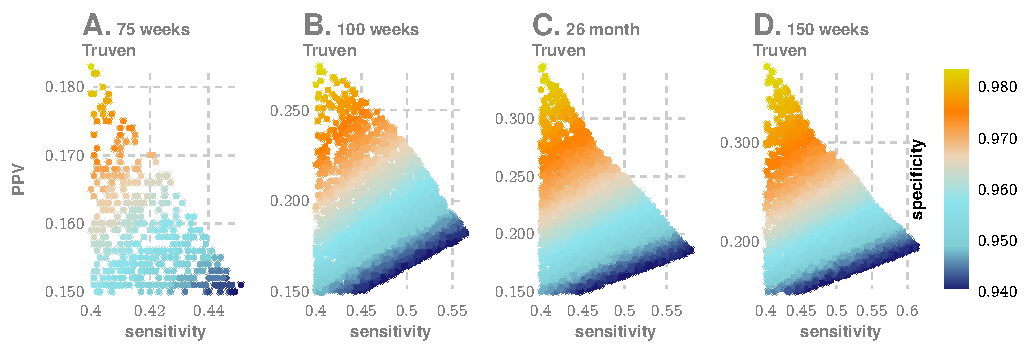
\includegraphics[width=0.9\textwidth]{Figures/External/4dopt}
  \fi 

\captionN{\textbf{4D Search To Take Advantage of Data on Population Stratification (Using Prevalence of 2.23\% as reported by CHOP~\cite{pmid31562252}).} While as  a standalone tool our approach is comparable to M-CHAT/F at around the 26 month mark (and later), we can take advantage of the independence of the tests to devise a conditional choice of the operating parameters for the new approach. In particular, taking advantage of published estimated prevalence rates of different categories of  M-CHAT/F scores, and  true positives in each sub-population upon stratification, we can choose a different set of specificity and sensitivity in each sub-population to yield significantly improved overall performance across databases, and much earlier. Additionally, we can choose to operate at a high recall point, where we maximize overall sensitivity, or a high precision point, where we maximize the positive predictive value.} \label{EXT-fig4D}
\end{figure*}
\else
\refstepcounter{figure}\label{EXT-fig4D}
\fi
%###########################################################
%###############################################

Assume that there are $m$ sub-populations such that:
the total number of positives and negatives, and the  prevalences in each sub-population are given by $P_i,N_i$ and $\rho_i$ respectively, with $ i \in \{1,\cdots, m\}$. Let $\beta_i$ be the relative size of the sub-populations. Thus, we have:
\cgather{
  P = \sum_i P_i\\
  N= \sum_i N_i\\
\beta_i = \frac{N_i+P_i}{N+P} \\
  \rho_i = \frac{P_i}{N_i + P_i}= \frac{P_i}{\beta_i(N + P)}
}%
Therefore, denoting the sensitivity and specificity of the sub-populations as $s_i$ and $c_i$ respectively, we have:
\cgather{
s=t_p/P = \frac{\sum_i t_p\vert_i}{P} = \frac{\sum_i (t_P\vert_i / P_i ) \times (\beta_i \rho_i (P+N))}{P} =\sum_i s_i \beta_i \frac{\rho_i}{\rho} 
}%
Thus, we end up with:
\begin{subequations}\label{eqscpop}
\cgather{
  s= \sum_{i=1}^m s_i \gamma_i  \\
  c= \sum_{i=1}^m c_i \gamma_i' \\
PPV = \frac{s}{s+(1-c)(\frac{1}{\rho} -1)}
\intertext{
where we have denoted:
}
\gamma_i = \beta_i \frac{\rho_i }{\rho}, \textrm{ and }  \gamma_i'= \beta_i \frac{1-\rho_i}{1-\rho}
  }%
\end{subequations}%
  Now, using Table~\ref{EXT-tabCHOP}, we can compute the values for $\gamma_i, \gamma_i'$, as shown below.

%#################################### 
\begin{table*}[!ht]
\centering

\mnp{.89\textwidth}{

\captionN{Boosted Sensitivity, Specificity and PPV Achieved at  \textbf{150 weeks}  Conditioned on M-CHAT/F Scores}\label{EXT-tabboost150}
  \vskip .5em

\begin{tabular} {L{.33in}|L{.33in}|L{.33in}|L{.33in}||L{.35in}|L{.35in}|L{.375in}||L{.375in}|L{.35in}|L{.35in}||L{.6in}}
\hline
\multicolumn{4}{c||}{\cellcolor{lightgray!60}M-CHAT/F Outcome}  & \multicolumn{3}{c||}{\mnp{.9in}{\vskip .2em global\\performance (Truven)\vskip .2em  } }&\multicolumn{3}{c||}{\mnp{1in}{\vskip .2em global\\performance\\(UCM)\vskip .2em }} &  \multirow{3}{*}{prevalence}\\\cline{0-9}
 0-2  NEG & 3-7  NEG & 3-7  POS & $\geq  8$  POS & \multirow{2}{*}{\mnp{.1in}{speci-ficity}} & \multirow{2}{*}{\mnp{.1in}{sensi-tivity}} &\multirow{2}{*}{PPV}& \multirow{2}{*}{\mnp{.1in}{speci-ficity}} & \multirow{2}{*}{\mnp{.1in}{sensi-tivity}} & \multirow{2}{*}{PPV} & \\\cline{0-3}
\multicolumn{4}{c}{\cellcolor{lightgray} specificity choices}  & & & &&&&\\\hline 
  0.28&0.66&0.93&0.97&0.95&0.64&0.224&0.95&0.577&0.206&0.022\\\hline 
0.31&0.67&0.9&0.97&0.95&0.641&0.223&0.95&0.577&0.205&0.022\\\hline 
0.54&0.86&0.97&0.99&0.98&0.494&0.361&0.98&0.393&0.31&0.022\\\hline 
0.41&0.89&0.96&0.99&0.98&0.493&0.362&0.98&0.391&0.311&0.022\\\hline 
0.31&0.61&0.86&0.98&0.95&0.808&0.219&0.95&0.713&0.198&0.017\\\hline 
0.33&0.6&0.86&0.98&0.95&0.809&0.218&0.95&0.715&0.197&0.017\\\hline 
0.66&0.95&0.98&0.99&0.98&0.574&0.337&0.98&0.417&0.269&0.017\\\hline 
0.53&0.97&0.98&0.99&0.98&0.573&0.337&0.98&0.412&0.267&0.017\\\hline 
0.54&0.91&0.97&0.99&0.978&0.615&0.322&0.978&0.499&0.278&0.017\\\hline 
0.52&0.92&0.97&0.99&0.978&0.612&0.324&0.978&0.492&0.278&0.017\\\hline 
 
\end{tabular}}

\vspace{5pt}

\mnp{.97\textwidth}{
  \captionN{Population Stratification Results on large M-CHAT/F Study(n=20,375)~\cite{pmid31562252} }\label{EXT-tabCHOP}
    \vskip .5em

  \begin{tabular}{C{.5in} | L{1.5in}|L{1in}|L{1in}|L{1in}||L{.5in}}\hline
 \bf \sffamily   Id &  \bf \sffamily Sub-population & \bf \sffamily Test Result & \bf \sffamily ASD positive & \bf \sffamily ASD Negative & \bf \sffamily Total \% \\\hline
   A &  M-CHAT/F $\geqq 8$ & Positive & 0.34\% & 0.64\% & 0.99\% \\\hline
  B &   M-CHAT/F $\in [3,7]$ & Positive (after follow-up)& 0.52\% & 4.39\% & 4.91\% \\\hline
 C &    M-CHAT/F $\in [3,7]$ & Negative (after follow-up)& 0.14\% & 3.1\% & 3.24\% \\\hline
  D &   M-CHAT/F $\in [0,2] $ & Negative & 1.22\% & 89.63\% & 90.86\% \\\hline\hline
    Total \%& &   &2.23\% & 97.77\% & 100\% \\\hline
    \end{tabular}
}

\vspace{5pt}

\mnp{.9\textwidth}{
  \captionN{$\gamma,\gamma'$ Computed from Population Stratification Recorded In  M-CHAT/F Study~\cite{pmid31562252} ($\rho=0.0223$) }\label{EXT-tabCHOP2}
    \vskip .5em

  \begin{tabular}{C{.5in} | L{1.35in} | L{1.5in}|L{.35in}|L{.35in}|L{.35in}|L{.35in}}\hline
 \bf \sffamily   Id  &  \bf \sffamily Sub-population& \bf \sffamily Test Result & $\beta_i$ & $\rho_i$ & \bf \sffamily $\gamma_i$ & \bf \sffamily $\gamma'_i$ \\\hline
   A & M-CHAT/F $\geqq 8$ &  Positive &.0099 & .3469 &.1540  & .0066 \\\hline
  B & M-CHAT/F $\in [3,7]$ & Positive (after follow-up)& .0491 & .1059 &.2331  & .0449 \\\hline
 C &   M-CHAT/F $\in [3,7]$ & Negative (after follow-up)& .0324 & .0432 &.0627  & .0317 \\\hline
  D &  M-CHAT/F $\in [0,2] $ & Negative & .9086 & .0134 &.5471  & .9168 \\\hline
    \end{tabular}}

\end{table*}
%###############################################
%###############################################

Using the prevalence and stratification parameters calculated from the CHOP study (See main text  Table~\ref{EXT-tabCHOP2}~\cite{pmid31562252}), we can compute a conditional choice of sensitivity and specificity for our tool, in each sub-population to ultimately yield an overall performance significantly  superior to  M-CHAT/F. We carry out a four-dimensional search at the age the CHOP population stratification is reported ($26$ months or 112 weeks approximately) to  identify the feasible region with  PPV  $>14.6\%$, or sensitivity  $>38.8\%$ while keeping specificity  $>94.9\%$ where each of these dimensions represent the independent choice of sensitivity in the corresponding sub-population. For each set of 4 choices, the corresponding specificities are read-off from our computed ROC curve, and then the overall sensitivity, specificity and PPV are calculated using Eq.~\eqref{eqscpop}. The results are shown in Fig.~\ref{EXT-fig4D}, where we include the computations at $75$ weeks, $125$ weeks, and $150$ weeks, with the same population stratification (although understandably the stratification will deviate from the values obtained at 26 months for those other ages).

An important assumption here is that the two tests are independent. Since M-CHAT/F is based on the detection of behavioral signals of developmental delay associated with autism via questionnaires completed by the primary care-givers, while our pipeline is based on  physical comorbidities, independence is reasonable. Hence, we can simulate the application of the pipeline to each sub-population, and compute the overall performance quantities using a pre-computed ROC curve. Here we use the curve corresponding to the age in weeks, but average the male and female ROC curves, which are  close as shown in Fig.~\ref{main-fig1} in the main text. The male-female averaging is necessary since the results from the CHOP study does not report sex stratified data.
 
We show the feasible region obtained by this computation in Fig.~\ref{EXT-fig4D} of this document, and in main text Fig.~\ref{main-figprc} of the main text. Particularly, note that we get a PPV close to or higher than $30\%$ at the high precision (HP) operating point, or a sensitivity above  55\% for the high recall (HR) operating point, when we restrict specificities to above $95\%$.
  
It is important to note  that Eq.~\eqref{eqscpop} and hence the results are dependent on the population prevalence $\rho$. We report the dependence of the solution to the 4D optimization for population prevalence between $1.7\%$ (CDC estimate~\cite{hyman2020identification}), and $2.23\%$ (CHOP estimate~\cite{pmid31562252}).
In particular, it is illuminating to compare these results directly with M-CHAT/F performance, as shown in Fig.~\ref{main-figprc}, panels B and C in the main text. In panel C, we show that for any stable population prevalence between  
$1.7\%$ and $2.24\%$, we can achieve nearly double the PPV without losing sensitivity, or increase the sensitivity by about 50\% without sacrificing PPV, while holding not letting the  specificity to drop below $94\%$.


\section{Generating PFSA Models From Set of Input Streams with Variable Input Lengths}\label{sec:varl}
Our PFSA reconstruction algorithm~\cite{CL12g} is distinct from standard HMM learning. We do not need to pre-specify structures, or the number of states in the algorithm, and all model parameters are inferred directly from data. Additionally, we can operate either  with 1) a single input stream, or  2) a set of input streams of possibly varying lengths which are assumed to be different and independent sample paths from the unknown stochastic generator we are trying to infer. At an intuitive level, we use the input data to infer the length of histories one must remember to estimate the current state, and predict futures for the process being modeled. Thus, we do not step     through the symbol streams with a pre-specified model structure, and  avoid the need to have equal-length inputs. More details of the algorithm are provided in the next section.

The ability to model a set of input streams of varying lengths is particularly important, since medical histories of different patients are typically of different lengths.

\DeclarePairedDelimiter{\ceil}{\lceil}{\rceil}
\renewcommand{\ceil}[1]{\left\lceil{#1}\right\rceil}

\section{Probabilsitic Finite State Automata Inference}
\label{sec:PFSA}

\subsection{Probabilistic Finite-State Automaton}
\label{subsec:DEFN_PFSA}
Let $\Sigma$ be a finite alphabet of symbols with size $\abs{\Sigma}$. The set of sequences of length $d$ over $\Sigma$ is denoted by $\Sigma^d$. The set of finite but unbounded sequences over $\Sigma$ is denoted by $\Sigma^\star$, the Kleene star operation \cite{hopcroft2008introduction}, \ie~$\Sigma^{\star} = \bigcup_{d=0}^{\infty}\Sigma^{d}$. We use lower case Greek, for example $\sigma$ or $\tau$, for symbols in $\Sigma$, and lower case Latin, for example $x$ or $y$, for sequences of symbols, \ie~$x=\sigma_1\sigma_2\dots\sigma_n$. We use $\abs{x}$ to denote the length of $x$.  The empty sequence is denoted by $\lambda$. 

We denote the set of strictly infinite sequences over $\Sigma$ by $\Sigma^\omega$, and the set of strictly infinite sequences having $x$ as prefix by $x\Sigma^\omega$. Let $\SR = \set{x\Sigma^\omega: x \in \Sigma^\star}\cup\set{\emptyset}$, we can verify that $\SR$ is a semiring \cite{klenke2013probability} over $\Sigma^{\omega}$. We use $\mathcal{F}$ to denote the sigma algebra generated by $\mathcal{S}$.

\begin{defn}[Stochastic Process over $\Sigma$]
\label{defn:StochasticProcessOverSigma}
A stochastic process over a finite alphabet $\Sigma$ is a collection of $\Sigma$-valued random variables $\set{X_t}_{t\in\mathbb{N}}$ indexed by positive integers~\cite{doob1990stochastic}.
\end{defn}
We are specifically interested in processes in which the $X_i$s are not necessarily independently distributed.

\begin{defn}[Sequence-Induced Measure and Derivative]
\label{defn:MeasureAndDeriv}
For a process $\mathscr{P}$, let $Pr_{\mathcal{P}}(x)$ or simply $Pr(x)$ denote the probability $\mathscr{P}$ producing a sample path prefixed by $x$. The \textbf{measure $\mu_x$ induced by a sequence $x\in \Sigma^{\star}$} is the extension \cite{klenke2013probability} to $\mathcal{F}$ of the premeasure defined on the semiring $\SR$ given by
\cgather{
%\label{eq:DefinitionOfPremeasure}
 \forall x,y\in\Sigma^{\star},   \mu_x\paren{y\Sigma^{\omega}} \triangleq \frac{Pr\paren{xy}}{Pr(x)}, \textrm{ if } Pr(x) > 0
}For any $d\in\mathbb{N}$, the \textbf{$d$-th order derivative} of a sequence $x$, written as $\phi^{d}_{x}$, is defined to be the marginal distribution of $\mu_{x}$ on $\Sigma^d$, with the entry indexed by $y$ denoted by $\phi^{d}_{x}(y)$. The first-order derivative is called the \textbf{symbolic derivative} and is denoted by $\phi_{x}$ for short.
\end{defn}

\begin{defn}[Probabilistic Nerode Equivalence and Causal States \cite{chattopadhyay2008structural}]
\label{defn:NerodeEquiv}
For any pair of sequences $x, y\in\Sigma^{\star}$, $x$ is equivalent to $y$, written as $x\sim y$, if and only if either $Pr(x) = Pr(y) = 0$, or $\mu_x = \mu_y$. The equivalence class of a sequence $x$ is denoted by $[x]$ and is called a \textbf{causal state} \cite{chattopadhyay2014data}. The cardinality of the set of causal states is called the \textbf{probabilistic Nerode index}, or the Nerode index for simplicity.
\end{defn}
We can see from the definition that causal states captures how the history of a process influences its future. Since the probabilistic Nerode equivalence is right invariant, it gives rise naturally to a automaton structure introduced below.

\begin{defn}[Probabilistic Finite-State Automaton (PFSA)]
\label{defn:PFSA}
A PFSA $G$ is defined by a quadruple $\paren{Q, \Sigma, \delta, \pitilde}$, where $Q$ is a finite set, $\Sigma$ is a finite alphabet, $\delta: Q\times\Sigma \rightarrow \Sigma$ is called the transition map, and $\pitilde: Q \rightarrow \mathbf{P}_\Sigma$, where $\mathbf{P}_\Sigma$ is the space of probability distributions over $\Sigma$, is called the transition probability. The entry of $\pitilde(q)$ indexed by $\sigma$ is denoted by $\pitilde(q,\sigma)$. 
\end{defn}
\begin{defn}[Transition and Observation Matrices]
The transition matrix $\Pi$ is the $|Q|\times|Q|$ matrix with the entry indexed by $q, q'$, written as $\pi_{q, q'}$, satisfying
\cgather{
    \pi_{q, q'} \triangleq \sum_{\mathclap{\set{\sigma\in\Sigma| \delta(q, \sigma) = q'}}}\pitilde(q, \sigma)
}and the observation matrix $\Pitilde$ is a $|Q|\times|\Sigma|$ matrix with the entry indexed by $q, \sigma$ equaling $\pitilde(q, \sigma)$.
\end{defn}
We note that both $\Pi$ and $\Pitilde$ are stochastic, \ie~non-negative with rows summing up to $1$. 
%
\begin{defn}[Extension of $\delta$ and $\pitilde$ to $\Sigma^{\star}$]
For any $x = \sigma_1\dots\sigma_k$, $\delta(q, x)$ is defined recursively by 
\cgather{
    \delta(q, x) \triangleq \delta\paren{\delta\paren{q, \sigma_1\dots\sigma_{k-1}}, \sigma_k}
}with $\delta(q, \lambda) = q$, and $\pitilde(q, x)$ is defined recursively by
\cgather{
    \pitilde(q, x) \triangleq \prod_{i=1}^{k}\pitilde\paren{\delta\paren{q, \sigma_1\dots\sigma_{i-1}}, \sigma_i}
}with $\pitilde(q, \lambda) = 1$. 
\end{defn}
%
\begin{defn}[Strongly Connected PFSA]
\label{defn:StrongConn}
We say a PFSA is strongly connected if the underlying directed graph is strongly connected \cite{bondy2008graph}. More precisely, a PFSA $G = \paren{Q, \Sigma, \delta, \pitilde}$ is strongly connected if for any pair of distinct states $q$ and $q'\in{Q}$, there is an $x\in\Sigma^{\star}$ such that $\delta(q, x) = q'$.
\end{defn}
We assume all PFSA in the discussions in the sequel are strongly connected if not specified otherwise. For strongly connected PFSA $G$, there is a unique probability distribution over $Q$ that satisfies $\mathbf{v}^{T}\Pi = \mathbf{v}^{T}$. This is  the \textbf{stationary distribution} \cite{vidyasagar2014hidden,kai1967markov_stdis} of $G$ and is denoted as $\wp_G$, or $\wp$ if $G$ is understood. 

\begin{defn}[$\Gamma$-Expression]
\label{defn:GammaExpr}
We can encode the information contained in $\delta$ and $\pitilde$ by a set of $|Q| \times |Q|$ matrices $\boldsymbol{\Gamma} = \set{\Gamma_\sigma| \sigma\in\Sigma}$, where
\cgather{
    \Gamma_\sigma\big|_{q, q'} \triangleq \left\{
        \begin{array}{ll}
        \pitilde(q, \sigma) & \textrm{if } \delta(q, \sigma) = q',\\
        0 & \textrm{if otherwise}.
        \end{array}\right.
}$\Gamma_\sigma$ is called \textbf{event-specific transition matrix}, with the event being that $\sigma$ is current the output. $\Gamma_\sigma$ can also be extended to arbitrary $x\in\Sigma^{\star}$ by defining $\Gamma_{x} = \prod_{i = 1}^{k}\Gamma_{\sigma_i}$ with $\Gamma_{\lambda} = I$.
\end{defn}
 
\begin{defn}[Sequence-Induced Distribution on States]
\label{defn:InducedDistr}
For a PFSA $G = \paren{Q, \Sigma, \delta, \pitilde}$ and a distribution $\wp_0$ on $Q$, the \textbf{distribution on $Q$ induced by a sequence $x$} is given by $\wp^{T}_{G, \wp_0}(x) = \nrm{\wp_0^{T}\Gamma_{x}}$ with $\wp_{G, \wp_0}(\lambda) = \wp_0$. The entry indexed by $q\in Q$ of the vector $\wp_{G, \wp_0}(x)$ is written as $\wp_{G, \wp_0}(x, q)$. When $\wp_0=\wp_{G}$, the stationary distribution of $G$, we write $\wp_{G, \wp_0}(x)$ as $\wp_{G}(x)$, or simply as $\wp(x)$, if $G$ is understood.
\end{defn}

\begin{defn}[Stochastic Process Generated by a PFSA]
\label{defn:StochasticProcessOfPFSA}
Let $G=\paren{Q, \Sigma, \delta, \pitilde}$ be a PFSA and let $\wp_0$ be a distribution on $Q$, the $\Sigma$-valued stochastic process $\set{X_t}_{t\in\Sigma}$ generated by $G$ and $\wp_0$ satisfies that $X_1$ follows the distribution $\wp_0$ and $X_{t+1}$ follows the distribution $\wp_{G, \wp_0}\paren{X_{1}\cdots X_{t}}$ for $t\in\N$.
\end{defn}
For the rest of this paper, we will assume $\wp_0 = \wp_G$ if not specified otherwise. We can show that, when initialized with $\wp_G$, the process generated by a PFSA $G$ is stationary and ergodic. We also note the, for the process generate by $G$, we have $\phi_x = \wp_G(x)^{T}\Pitilde$. Since $\wp_G(\lambda) = \wp_{G}$, the symbolic derivative of the empty sequence $\phi_\lambda$ is the stationary distribution on the symbols. 

\begin{defn}[Synchronizable PFSA and Synchronizing Sequence]
A \textbf{synchronizing sequence} is a finite sequence that sends an arbitrary state of the PFSA to a fixed state \cite{trahtman2008road}. To be more precise, let $G=\paren{Q, \Sigma, \delta, \pitilde}$ be a PFSA, we say a sequence $x\in\Sigma^{\star}$ is a synchronizing sequence to a state $q \in Q$ if $\delta(q', x) = q$ for all $q'\in {Q}$. A PFSA is \textbf{synchronizable} if it has at least one synchronizing sequence. Given a sample path generated by a PFSA, we say the PFSA is \textbf{synchronized} if a synchronizing sequence transpires in the sample path.    
\end{defn}

\begin{defn}[Equivalence and Irreducibility]
Two PFSA $G$ and $H$ are \textbf{equivalent} if they generate the same stochastic process. A PFSA $G$ is said to be \textbf{irreducible}, if there is not another PFSA with smaller state set that is equivalent to $G$. 
\end{defn}
\begin{defn}
Consider a PFSA $G$ over state set $Q$. For a give $\varepsilon > 0$, we say a sequence $x$ is a $\varepsilon$-synchronizing sequence to a state $q\in Q$ if
\cgather{
    \norm{\wp_{G}(x) - \mathbf{e}_q}_{\infty} \leq \varepsilon. 
}
\end{defn}
While there exists PFSA that is not synchronizable, we can show that an irreducible PFSA always has an $\varepsilon$-synchronizing sequence for some state $q$ for arbitrarily small $\varepsilon > 0$. Moreover, we can show that as length increases, sequences produced by PFSA become uniformly $\varepsilon$-synchronizing. These two are the underpinning properties for the inference algorithm of PFSA (See Alg.~\ref{alg:GenESeSS}), because they imply that $\phi_x$ can be used to approximate $\pitilde(q)$ if $x$ are properly prefixed and long enough.

\begin{defn}[Joint $\varepsilon$-Synchronizing Sequence]
\label{def:JointSyncSeq}
Let $G$ and $H$ be two PFSA over state sets $Q_{G}$ and $Q_H$, respectively. For a fixed $\varepsilon$, a sequence $x$ is said to be \textbf{jointly $\varepsilon$-synchronizing} to $(q, r)\in{Q_{G}}\times Q_{H}$ if $x$ is $\varepsilon$-synchronizing to $q$ and to $r$ simultaneously. We define
\cgather{
    \Sigma^{d}_{\varepsilon, (q, r)} \triangleq \set{x\in\Sigma^{d}:\ \textrm{$x$ jointly $\varepsilon$-synchronizing to $(q, r)$}}
}
\end{defn}

\begin{defn}[Joint Pair of States]
Let $G$ and $H$ be two PFSA over state sets $Q_{G}$ and $Q_H$, respectively. Define
\cgather{
    p_{G}(q,r) \triangleq \lim_{d\rightarrow\infty}p_{G}\paren{\Sigma^{d}_{\varepsilon, (q,r)}}
}A pair of states $(q,r)\in Q_G\times Q_H$ is called a \textbf{$G$-joint pair} of states if $p_{G}(q,r) > 0$. We also define
\cgather{
    Q_\textrm{c} \triangleq \set{(q, r)\in Q_G \times Q_H:\ \textrm{$(q, r)$ is a $G$-joint pair}}
}
\end{defn}


The inference algorithm for PFSA is called \textbf{\algo} for \underline{Gen}erator \underline{E}xtraction Using \underline{Se}lf-\underline{s}imilar \underline{S}emantics. With an input sequence $x$ and a hyperparameter $\varepsilon$, \algo outputs a PFSA in the following three steps: 1) approximate an almost synchronizing sequence; 2) identify the transition structure of the PFSA; 3) calculate the transition probabilities of the PFSA. See Alg.~\ref{alg:GenESeSS} for detail.
\begin{algorithm}[!ht]
    \KwData{A sequence $x$ over alphabet $\Sigma$, $0< \varepsilon < 1$}
    \KwResult{State set $Q$, transition map $\delta$, and transition probability $\pitilde$}
    \tcc{\textcolor{PineGreen}{\textbf{Step One: Approximate $\varepsilon$-synchronizing sequence}}}
    Let $L=\ceil{\log_{\abs{\Sigma}}1/\varepsilon}$\; \label{alg:GenL}
    Calculate the \textbf{derivative heap} $\mathcal{D}^{x}_{\varepsilon}$ equaling $\set{\hat{\phi}^{x}_y\ :\ \textrm{$y$ is a sub-sequence of $x$ with } |y|\leq L}$\;
    Let $\mathcal{C}$ be the convex hull of $D^{x}_{\varepsilon}$\; \label{alg:GenConv}
    Select $x_0$ with $\hat{\phi}^{x}_{x_0}$ being a vertex of $\mathcal{C}$ and has the highest frequency in $x$\; \label{alg:GenSyncSeq}
    \tcc{\textcolor{PineGreen}{\textbf{Step Two: Identify transition structure}}}
    Initialize $Q = \set{q_0}$\; \label{alg:GenStep2Start}
    Associate to $q_0$ the \textbf{sequence identifier} $x^{\textrm{id}}_{q_0} = x_0$ and the probability vector $d_{q_0} = \hat{\phi}^x_{x_0}$\;
    Let $\widetilde{Q}$ be the set of states that are just added and initialize it to be $Q$\;
    \While{$\widetilde{Q}\neq\emptyset$}{
        Let $Q_\textrm{new} = \emptyset$ be the set of new states\;
        \For{$(q, \sigma)\in \widetilde{Q} \times \Sigma$}{
            Let $x = x^{\textrm{id}}_q$ and $d = \hat{\phi}^x_{x\sigma}$\;
            \eIf{$\norm{d-d_{q'}}_\infty < \varepsilon$ for some $q'\in Q$\label{alg:GenIdenStateStart}}{
                Let $\delta(q, \sigma) = q'$\;
            }{
                Let $Q_\textrm{new} = Q_\textrm{new}\cup\set{q_\textrm{new}}$ and $Q = Q\cup\set{q_\textrm{new}}$\;
                Associate to $q_\textrm{new}$ the sequence identifier $x_{q_\textrm{new}}^{\textrm{id}} = x\sigma$ and the probability vector $d_{q_\textrm{new}}=d$\;
                Let $\delta(q, \sigma) = q_\textrm{new}$\;
            }\label{alg:GenIdenStateEnd}
        }
        Let $\widetilde{Q} = Q_{\textrm{new}}$\;
    }
    Take a strongly connected subgraph of the labeled directed graph defined by $Q$ and $\delta$, and denote the vertex set of the subgraph again by $Q$\;\label{alg:GenStep2End}
    \tcc{\textcolor{PineGreen}{\textbf{Step Three: Identify transition probability}}}
    Initialize counter $N\bracket{q,\sigma}$ for each pair $(q, \sigma) \in Q\times\Sigma$\; \label{alg:GenIdenTransProbStart}
    Choose a random starting state $q\in Q$\;
    \For{$\sigma\in x$}{
        Let $N\bracket{q,\sigma} = N\bracket{q,\sigma} + 1$\;
        Let $q = \delta\paren{q,\sigma}$\;
    }
    Let $\pitilde\paren{q} = \nrm{\paren{N\bracket{q,\sigma}}_{\sigma\in\Sigma}}$\;\label{alg:GenIdenTransProbEnd}
    \Return $Q$, $\delta$, $\pitilde$\;
    \caption{\algo}
    \label{alg:GenESeSS}
\end{algorithm}

\section{Sequence Likelihood Defect}
\label{sec:SLD}

\begin{defn}[Entropy Rate and KL Divergence]
By entropy rate of a PFSA, we mean the entropy rate of the stochastic process generated by the PFSA\cite{cover2012elements}. Similarly, by KL divergence of two PFSA, we mean the KL divergence between the two processes generated by them~\cite{matthews2016sparse}. More precisely, we have
\cgather{
    \mathcal{H}(G) = -\lim_{d\rightarrow\infty}\frac{1}{d}\sum_{x\in\Sigma^{d}}p(x)\log p(x)
}
and the KL divergence 
\cgather{
    \mathcal{D}_{\textrm{KL}}\parenBar{G}{H} = \lim_{d\rightarrow\infty}\frac{1}{d} \sum_{x\in\Sigma^{d}}p_{G}(x)\log\frac{p_{G}(x)}{p_{H}(x)}
}
whenever the limits exist.
\end{defn}

\begin{thm}[Closed-form Formula for Entropy Rate and KL Divergence]
\label{thm:Closed-formFormulaForEntropyRate}
The entropy rate of a PFSA $G = \paren{\Sigma, Q, \delta, \pitilde}$ is given by 
\cgather{
    \mathcal{H}(G) = \sum_{q\in{Q}}\wp_{G}(q)\cdot h(\pitilde(q))
}
where $h(\mathbf{v})$ is the based-$2$ entropy of the probability vector $\mathbf{v}$.

Consider two PFSA $G = \paren{Q_{\textrm{G}}, \Sigma, \delta_{G}, \pitilde_{G}}$ and $H = \paren{Q_{\textrm{H}}, \Sigma, \delta_{H}, \pitilde_{H}}$ with $\mu_{G}$ being absolutely continuous with respect to $\mu_{H}$. Let $Q_\textrm{c}$ be the set of $G$-joint pairs of states, we have
\cgather{
    \mathcal{D}_{\textrm{KL}}\parenBar{G}{H} = \sum_{(q,r)\in Q_\textrm{c}} p_{G}\paren{q, r}D_{KL}\parenBar{\pitilde_{G}(q)}{\pitilde_{H}(r)}
}
\end{thm}

\begin{defn}[Log-likelihood]
Let $x\in\Sigma^{d}$, the log-likelihood~\cite{cover2012elements} of a PFSA $G$ generating $x$ is given by
\cgather{
    L(x, G) = -\frac{1}{d}\log p_G(x)
}
\end{defn}
The calculation of log-likelihood is detailed in Alg.~\ref{alg:LLK}.
\begin{algorithm}[!ht]
    \KwData{A PFSA $G = \paren{\Sigma, Q, \delta, \pitilde}$ and a sequence $x$ over alphabet $\Sigma$}
    \KwResult{Log-likelihood $L(x, G)$ of $G$ generating $x$}

	Calculate the state transition matrix $\Pi$ and observation $\Pitilde$\; 
	Calculate the stationary distribution over states $\wp_{G}$ of $G$ from $\Pi$\;
	Calculate the stationary distribution of alphabet $\phi_{\lambda}^{T} = \wp_{G}^{T}\Pitilde$\;
	Initialize $\mathbf{p}$ by $\wp_{G}$ and $\mathbf{q}$ by $\phi_{\lambda}$\;
	Let $L = 0$\;
    \For{$i$ from $1$ to $|x|$}{
		Let $\sigma$ be the $i$-th entry of $x$\;
		Let $L = L - \log\mathbf{q}|_\sigma$\;
		Let $\mathbf{p}^{T} = \nrm{\mathbf{p}^{T}\Gamma_{\sigma}}$ where $\Gamma_{\sigma}$ is defined in \ref{defn:GammaExpr}\;
		Let $\mathbf{q}^{T} = \mathbf{p}^{T}\Pitilde$\;
    }
    \Return $L / |x|$;
    \caption{Log-likelihood}
    \label{alg:LLK}
\end{algorithm}

\begin{thm}[Convergence of log-likelihood]
\label{thm:convergenceOfLLH}
Let $G$ and $H$ be two reduced PFSA, and let $x\in\Sigma^d$ be a sequence generated by $G$. Then we have
\cgather{
    L(x, H)\rightarrow \mathcal{H}(G) + \mathcal{D}_{\textrm{KL}}\parenBar{G}{H}
}in probability as $d\rightarrow\infty$.
\end{thm}


\begin{proof}
We first notice that
\calign{
    \sum_{x\in\Sigma^{d}}p_{G}(x)\log\frac{p_{G}(x)}{p_{H}(x)} =& \sum_{x\in\Sigma^{d-1}}\sum_{\sigma\in\Sigma}p_{G}(x)\wp_{G}(x)\left.\Pitilde_{G}\right|_{\sigma}\log\frac{p_{G}(x)\wp_{G}(x)\left.\Pitilde_{G}\right|_{\sigma}}{p_{H}(x)\wp_{H}(x)\left.\Pitilde_{H}\right|_{\sigma}}\\
    =&\sum_{x\in\Sigma^{d-1}}p_{G}(x)\log\frac{p_{G}(x)}{p_{H}(x)} + \underbrace{\sum_{x\in\Sigma^{d-1}}p_{G}(x)\sum_{\sigma\in\Sigma}\wp_{G}(x)\left.\Pitilde_{G}\right|_{\sigma} \log\frac{\wp_{G}(x)\left.\Pitilde_{G}\right|_{\sigma}}{\wp_{H}(x)\left.\Pitilde_{H}\right|_{\sigma}}}_{D_d}
}By induction, we have $\mathcal{D}_{\textrm{KL}}\parenBar{G}{H} = \lim_{d\rightarrow\infty}\frac{1}{d}\sum_{i=1}^{d}D_{i}$, 
and hence by Ces\`{a}ro summation theorem \cite{hardy1992divergent}, we have $\mathcal{D}_{\textrm{KL}}\parenBar{G}{H} = \lim_{d\rightarrow\infty} D_d$. Let $x=\sigma_1\sigma_2...\sigma_n$ be a sequence generated by $G$. Let $x^{[i-1]}$ is the truncation of $x$ at the $(i-1)$-th symbols, we have
\calign{
    -\frac{1}{n}\sum_{i=1}^{n}\log\wp_{H}\paren{x^{[i-1]}}\left.\Pitilde_{H}\right|_{\sigma_i} = \underbrace{\frac{1}{n}\sum_{i=1}^{n}\log\frac{\wp_{G}\paren{x^{[i-1]}}\left.\Pitilde_{G}\right|_{\sigma_{i}}}{\wp_{H}\paren{x^{[i-1]}}\left.\Pitilde_{H}\right|_{\sigma_i}}}_{A_{x, n}} - \underbrace{\frac{1}{n}\sum_{i=1}^{n}\log\wp_{G}\paren{x^{[i-1]}}\left.\Pitilde_{G}\right|_{\sigma_i}}_{B_{x, n}}
}Since the stochastic process $G$ generates is ergodic, we have
\cgather{
    \lim_{n\rightarrow\infty}A_{x,n} = \lim_{d\rightarrow\infty}D_d = \mathcal{D}_{\textrm{KL}}\parenBar{G}{H}
}and $\lim_{n\rightarrow\infty}B_{x,n} = \mathcal{H}(G)$.
\end{proof} 



\section{Pipeline Optimization}\label{sec:pipeline}
% % ###########################
% \tikzexternalenable
% % ###########################
\subsection{Input Data Format}
\begin{algorithm}[!t]
    \SetAlgoLined
    \LinesNumbered
    
    \SetKwFunction{Dictionary}{Dictionary}
    \SetKwFunction{List}{List}
    \SetKwInOut{Input}{input}
    \SetKwInOut{Output}{output}
    
    \Input{Dataset, TargetDiseaseGroup, DiseaseGroups}
    \Output{Encoding} 
    \BlankLine
    Encoding $\leftarrow$ new  \Dictionary{}\;
    \For{$diseaseGroup \in DiseaseGroups$}{
        Encoding[diseaseGroup][patientID] $\leftarrow$ new \List{}\;
        Encoding[diseaseGroup][gender] $\leftarrow$ new \List{}\;
        Encoding[diseaseGroup][record] $\leftarrow$ new \List{}\;
        Encoding[diseaseGroup][target] $\leftarrow$ new \List{}\;
        \For{$record \in Dataset$}{
            \emph{//encode Dataset into a weekly trinary sequence}\;
            weeklyEncoding $\leftarrow$ new \List{}\;
            \For{$weeklyDiseaseRecord \in record$}{
                \emph{//no code recorded for the observed week}\;
                \If{$weeklyDiseaseRecord.code == NIL$}{
                    append "0" to weeklyEncoding\;
                }
                \If{$weeklyDiseaseRecord.code \in diseaseGroup.codes$}{
                    append "1" to weeklyEncoding\;
                }
                \If{$weeklyDiseaseRecord.code \notin diseaseGroup.codes$}{
                    append "2" to weeklyEncoding\;
                }
            }
            target $\leftarrow$ 1 if any weeklyDiseaseRecord.code of record $\in$ TargetDiseaseGroup\;
            \If{$target == 1$}{
                cut weeklyEncoding up to (but not including) first occurrence of TargetDiseaseGroup member\;
            }
            append record.patientID to Encoding[diseaseGroup][patientID]\;
            append record.gender to Encoding[diseaseGroup][gender]\;
            append weeklyEncoding to Encoding[diseaseGroup][record]\;
            append target to Encoding[diseaseGroup][target]\;
        }
    }
    \Return{Encoding}\;
    \caption{ICD-9 Encoding}\label{algo1}
\end{algorithm}


\begin{algorithm}[!t]
    \SetAlgoLined
    \LinesNumbered
    
    \SetKwFunction{Dictionary}{Dictionary}
    \SetKwFunction{List}{List}
    \SetKwFunction{Dataframe}{Dataframe}
    \SetKwFunction{TrainTestSplit}{TrainTestSplit}
    \SetKwFunction{genESeSS}{genESeSS}
    \SetKwFunction{ComputeSequenceFeature}{ComputeSequenceFeature}
    \SetKwFunction{llk}{llk}
    \SetKwFunction{pairwise}{pairwise}
    \SetKwFunction{outerjoin}{outerjoin}
    \SetKwFunction{LightGBM}{LightGBM}
    
    \SetKwInOut{Input}{input}
    \SetKwInOut{Output}{output}
    
    \Input{Encoding, DiseaseGroups, SequenceFeatures, hyperparameters}
    \Output{Predictions, FeatureImportances} 
    \BlankLine
    DiseaseDatasets $\leftarrow$ new  \Dictionary{}\;
    \For{$Dataset, DiseaseGroup \in zip(Encoding, DiseaseGroups)$}{
        PFSAset, LLset $\leftarrow$ \TrainTestSplit{Dataset, w.r.t = "target"}\;
        df $\leftarrow$ new \Dataframe{}\;
        df[patientID] $\leftarrow$ LLset[patientID]\;
        df[target] $\leftarrow$ LLset[target]\;
        \emph{//Generate 2 PFSAs for each class}\;
        PositivePFSAset $\leftarrow$ PFSAset[PFSAset.target == 1]\;
        NegativePFSAset $\leftarrow$ PFSAset[PFSAset.target == 0]\;
        PosPFSA $\leftarrow$ \genESeSS{PositivePFSAset}\;
        NegPFSA $\leftarrow$ \genESeSS{NegativePFSAset}\;
        \emph{//For each record, compute loglikelihoods of being generated by either of 2 PFSAs generated above}\;
        PosLLK $\leftarrow$ \llk{LLset, PosPFSA}\;
        NegLLK $\leftarrow$ \llk{LLset, NegPFSA}\;
        \emph{//Compute sequence likelihood defect}\;
        df[DiseaseGroup] $\leftarrow$ \pairwise{PosLLK - NegLLK}\;
        df[DiseaseGroup + '\_abs\_neg'] $\leftarrow$ NegLLK\;
        \For{$SequenceFeature \in SequenceFeatures$} { 
            df[DiseaseGroup + '\_' +  SequenceFeature] $\leftarrow$ [\ComputeSequenceFeature{SequenceFeature, seq} for each seq $\in$ LLset['record']]\;
        }
        DiseaseDatasets[DiseaseGroup] $\leftarrow$ df\;
    }
    Dataset $\leftarrow$ \outerjoin{DiseaseDatasets.values, on = 'patientID'}\;
    Aggregate all features in Dataset where feature\_name $\in$ DiseaseGroups (mean, std. deviation, range)\;
    Aggregate all features in Dataset where feature name minus '\_abs\_neg' $\in$ DiseaseGroups (mean, std. deviation, range)\;
    Aggregate all sequence features in Dataset (mean, std. deviation, range, max)\;
    TrainSet, TestSet $\leftarrow$ \TrainTestSplit{Dataset, w.r.t = "target"}\;
    LGBM $\leftarrow$ new \LightGBM{hyperparameters}\;
    LGBM.fit(TrainSet)\;
    Predictions $\leftarrow$ LGBM.predict(TestSet)\;
    \Return{Predictions, LGBM.feature\_importances}\;
    \caption{Prediction Pipeline Training}\label{algo2}
\end{algorithm}
% \begin{figure}[!ht]
%   \centering
  
%   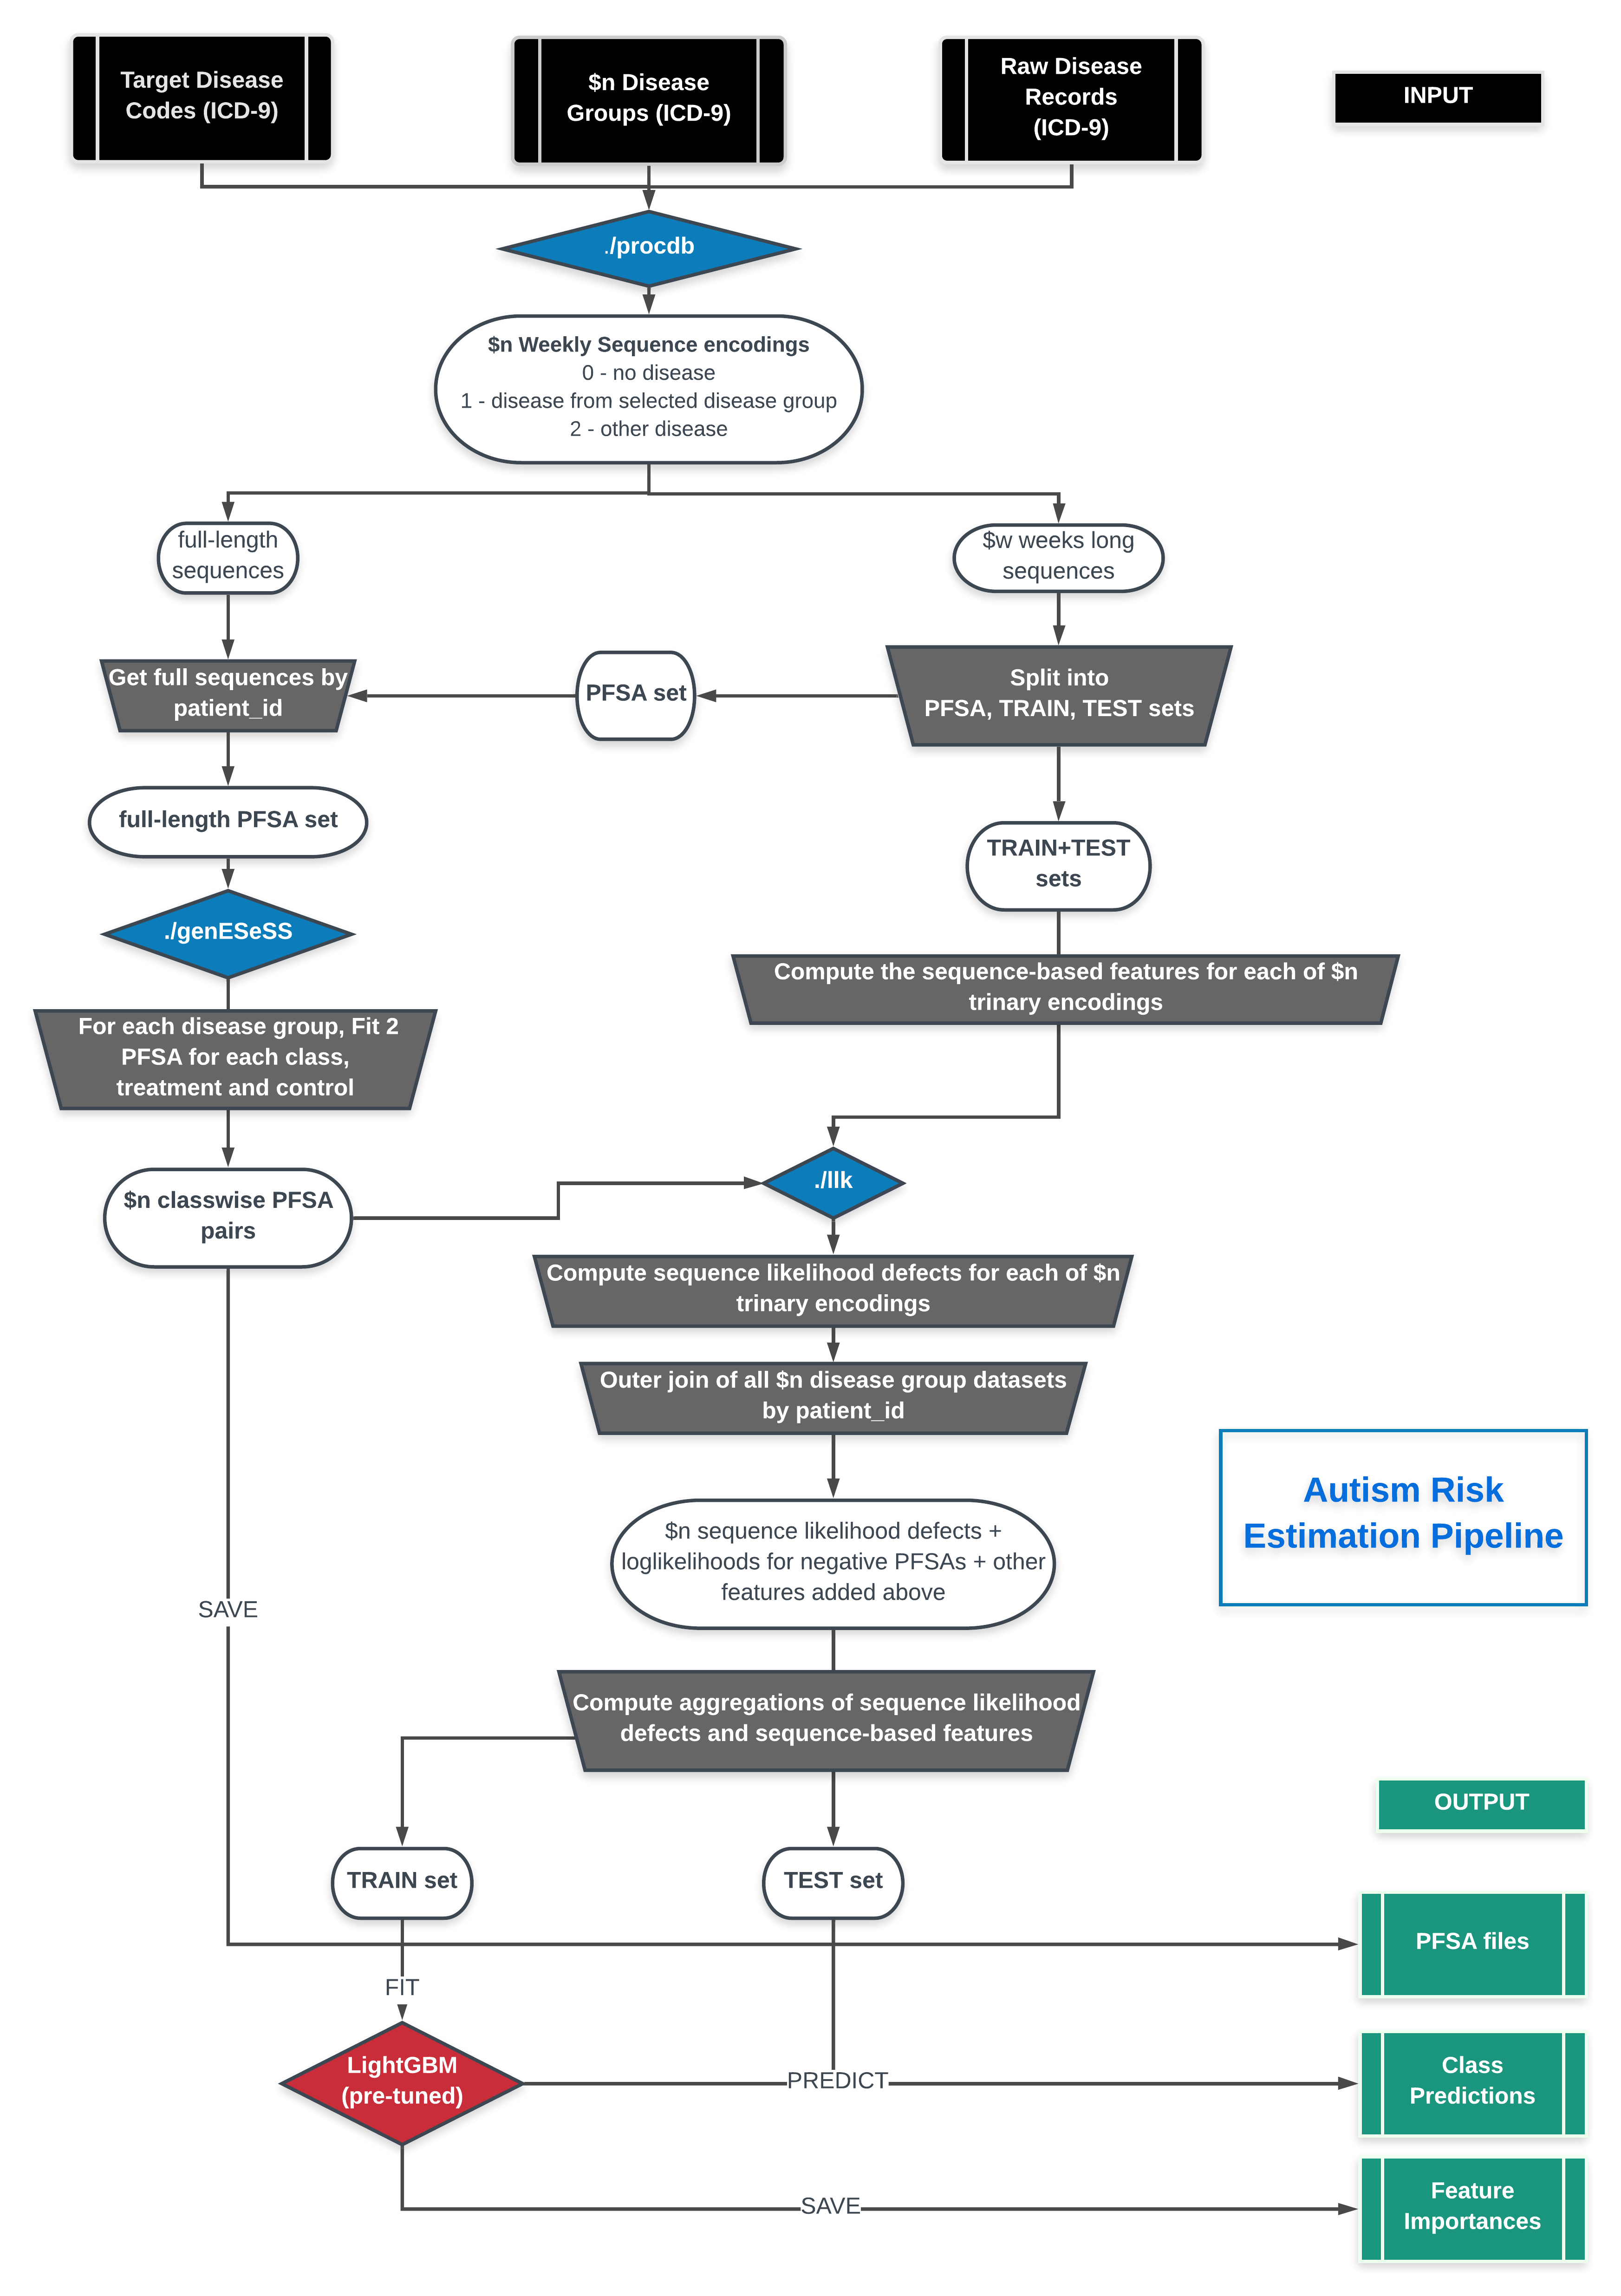
\includegraphics[width=\textwidth]{Figures/Pipeline}
%   \captionN{Pipeline schema: How the data set is split into test sets and two training sets: one for inferring HMM models, and one for training the boosting classifier.}\label{figschema}
%   \vspace{-20pt}
% \end{figure}


% Individual weekly medical history records, for a large cohort of US children between the years 2003 and 2010. The data is an excerpt from an insurance claims database tracking over 200 million people in US over a decade, with ICD-9 code representation of diseases. Each medical record is a list of ICD-9 codes with recorded week disease occurred.
% Records are classified by patient’s gender and county (FIPS code) of residence. The following pipeline works with two gender subsets of the input data separately.

To encode the ICD-9 codes, 17 Disease Groups of codes are used  to transform the raw health records into a format suitable for PFSA. As described in $Algorithm 1$, for each patient, the list of ICD-9 codes is encoded into a weekly array of three-symbol alphabet digits with respect to selected disease group, for each week: "0" - no disease "1" - disease from the selected group, "2" - other disease.

Once the trinary encodings are ready, the PFSA pairs are fit for each of the disease groups, on positive (treatment) and negative (control) sets using \texttt{genESeSS} algorithm~\cite{CL12g} (See Section~\ref{sec:PFSA}), as described in $Algorithm$ $2$. The PFSA pairs are then used to obtain the loglikelihood scores of belonging to a  PFSA modeling the positive and the control cohorts accordingly for each of the encodings of a patient record. As a result, we yield the difference between positive and control loglikelihoods for each disease group of each patient. The positive value of difference means that with respect to a given disease group, a certain patient is more likely to be a positive one. Conversely, the negative value of difference signifies that a patient is more likely to be from the control group. These features, as well as their aggregations and the aggregations of the ternary encoding arrays, are used as the features for the final  LightGBM gradient boosting classifier.

% \\
%%%%%%%%%%%%%%%%%%%%%%%%%%%%%%%%%%%%%%%%%%%%%%%%%%%%%%%%%%%%%%
\subsection{Algorithms}
The key data processing approach is outlined in Algorithm~\ref{algo1}. The remaining steps of the approach are sketched in Algorithm~\ref{algo2}. Fig.~\ref{figschema} shows the overall schema, including the breakdown of a database into a test set, and two training sets: one for training the HMM models, and one for training the boosting classifier.

\begin{figure}[!ht]
  \centering
  
  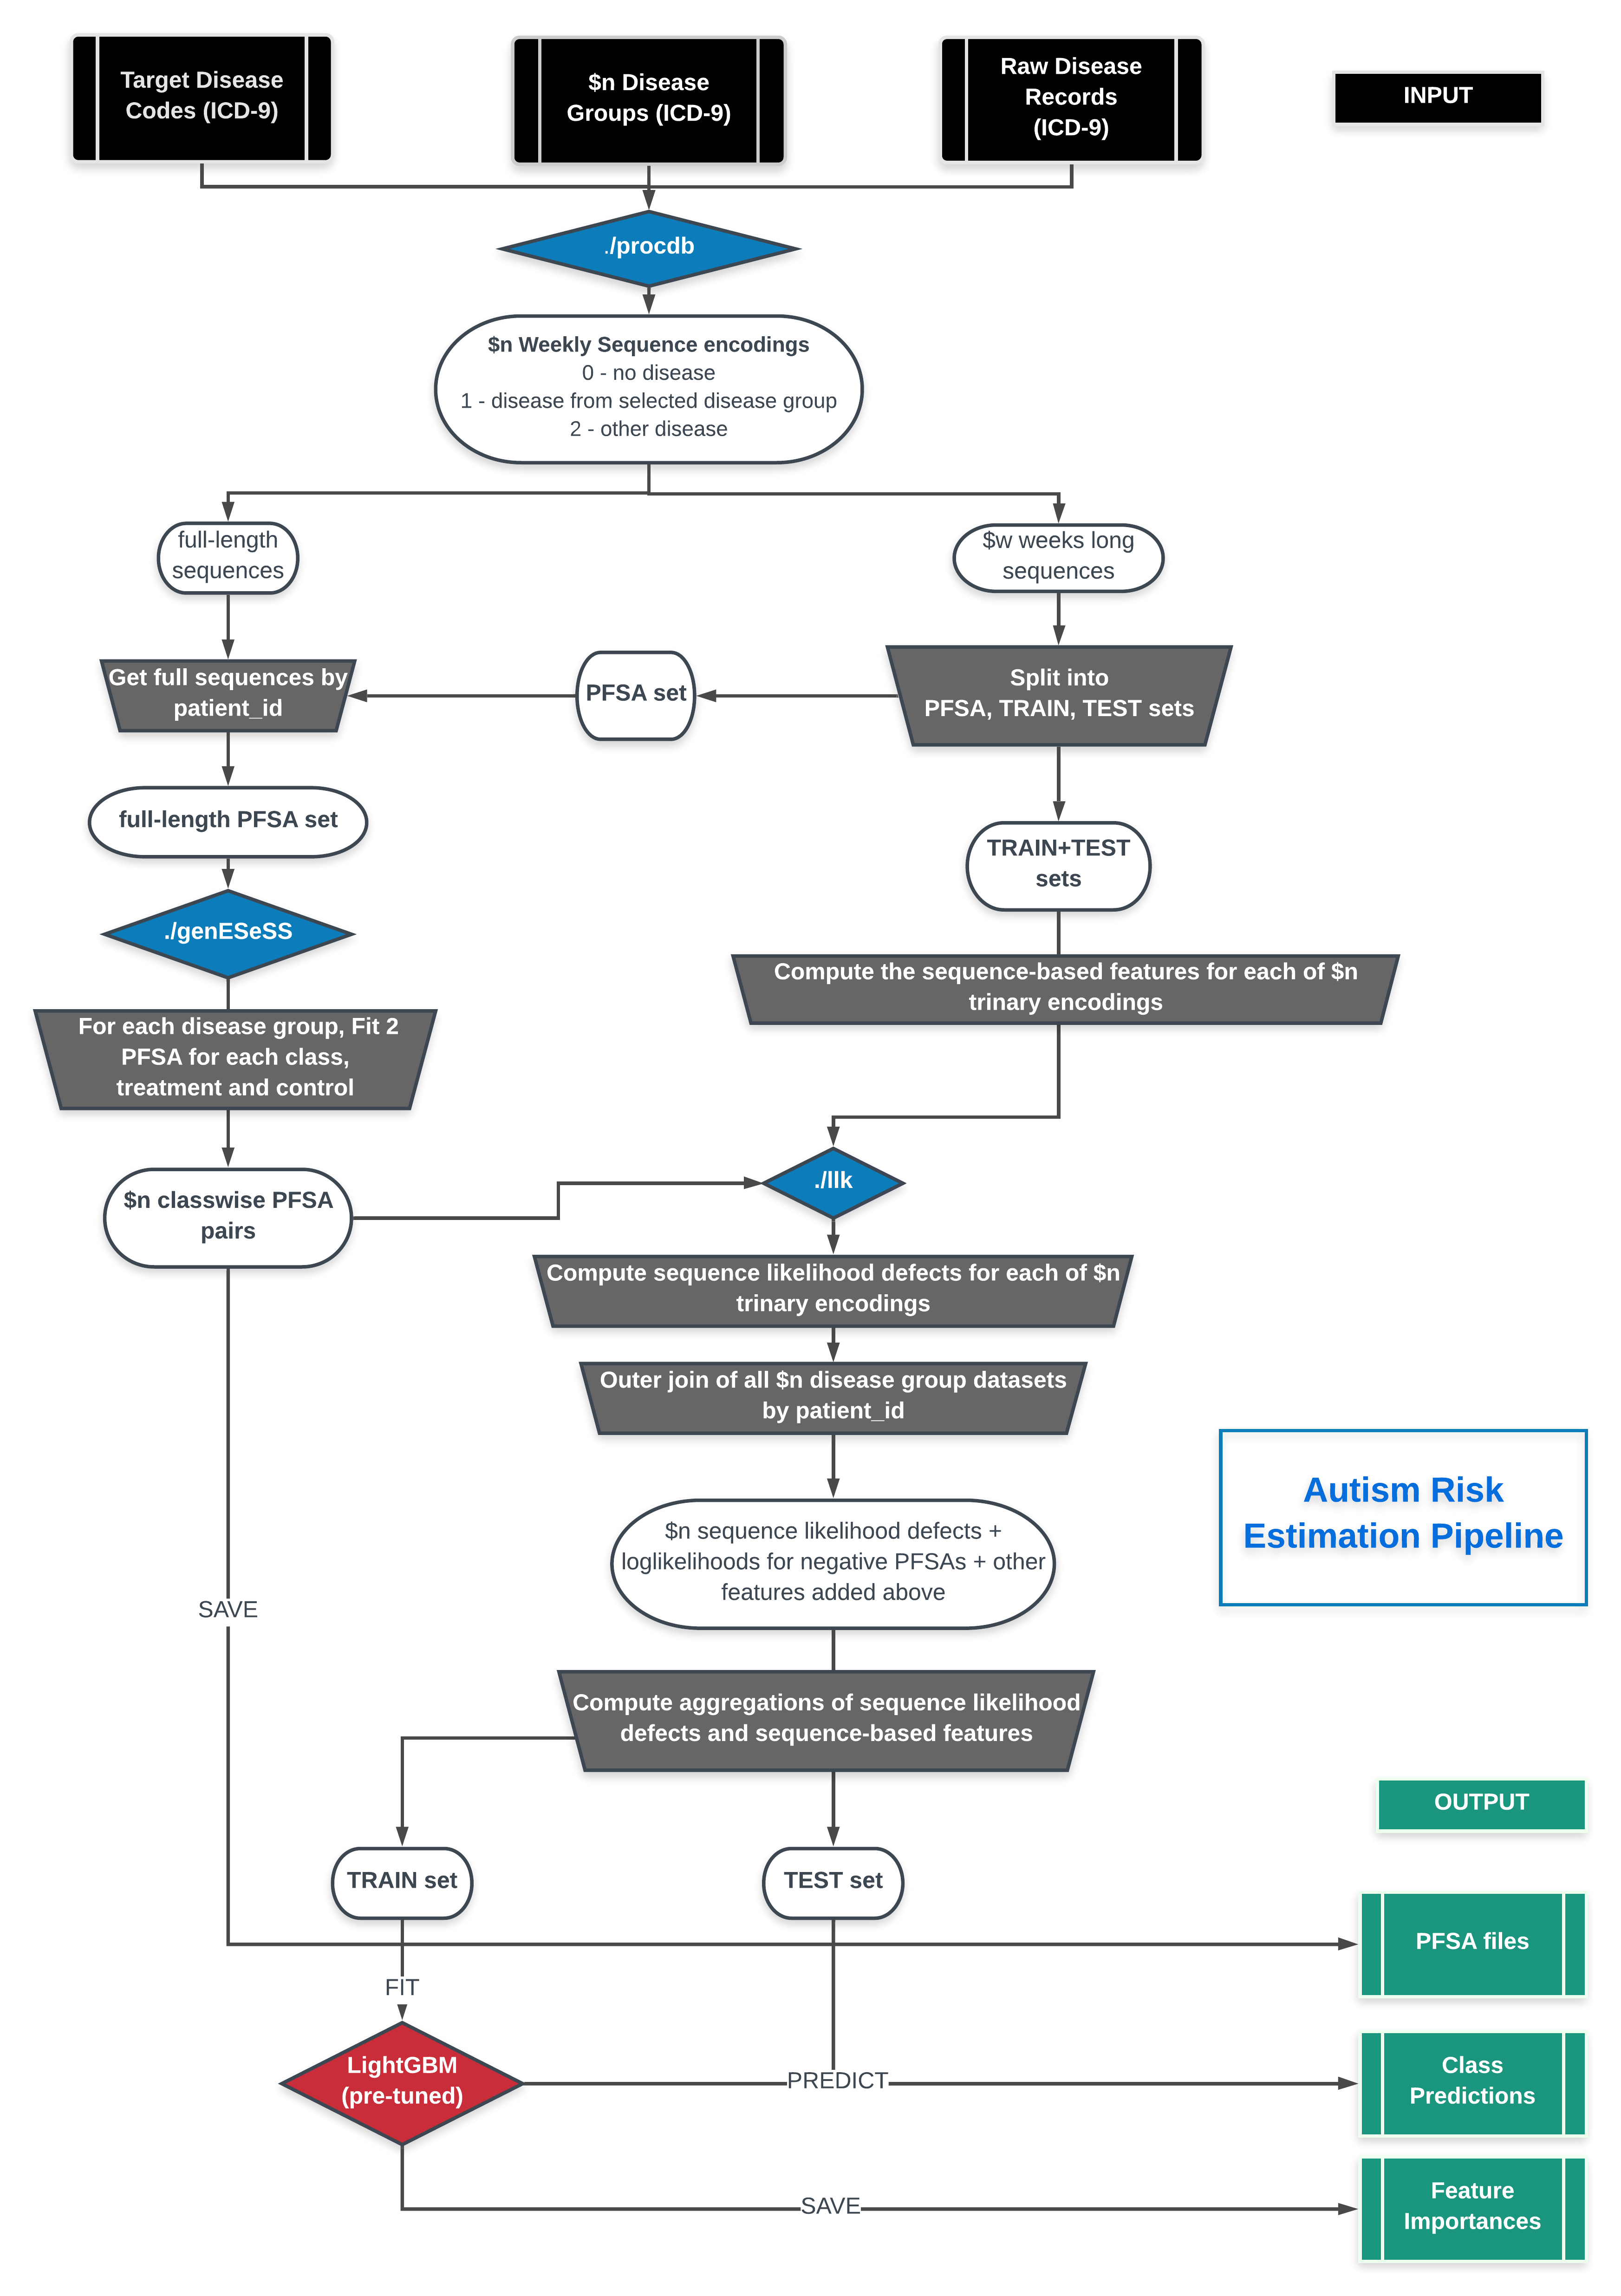
\includegraphics[width=.85\textwidth]{Figures/Pipeline}
  \captionN{Pipeline schema: How the data set is split into test sets and two training sets: one for inferring HMM models, and one for training the boosting classifier. The two key algorithms here are \texttt{genESeSS}~\cite{CL12g} and the llk which does the sequence likelihood computation described in Section~\ref{sec:SLD}}\label{figschema}
  \vspace{-20pt}
\end{figure}
%\clearpage
\section{Example Run with Released  Application}\label{sec:app}

%###################################
%###################################
%###################################
\begin{figure}[!ht]
\centering
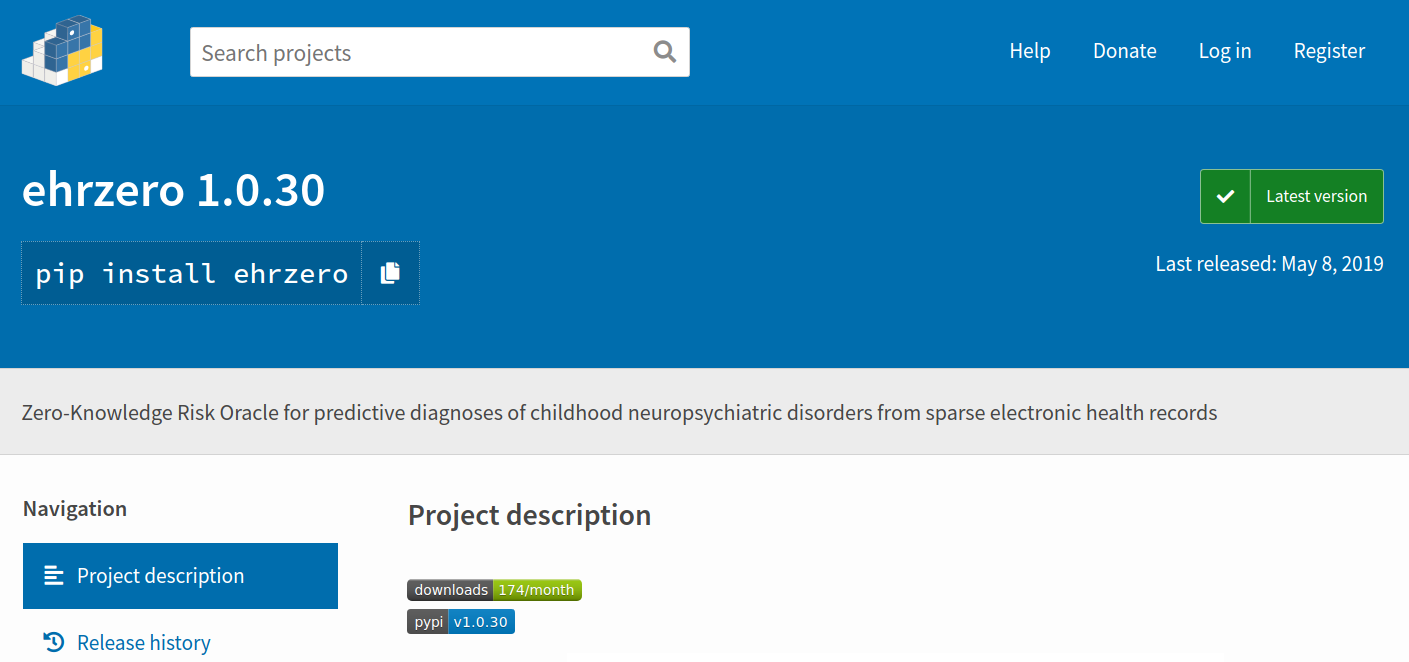
\includegraphics[width=.9\textwidth]{Figures/scrn}
\captionN{Screen capture of the page on pypi.org hosting the released application Link: \href{hhtp://pypi.org/ehrzero}{http://pypi.org/ehrzero}}
\end{figure}
%###################################

\begin{figure}[!ht]
\centering
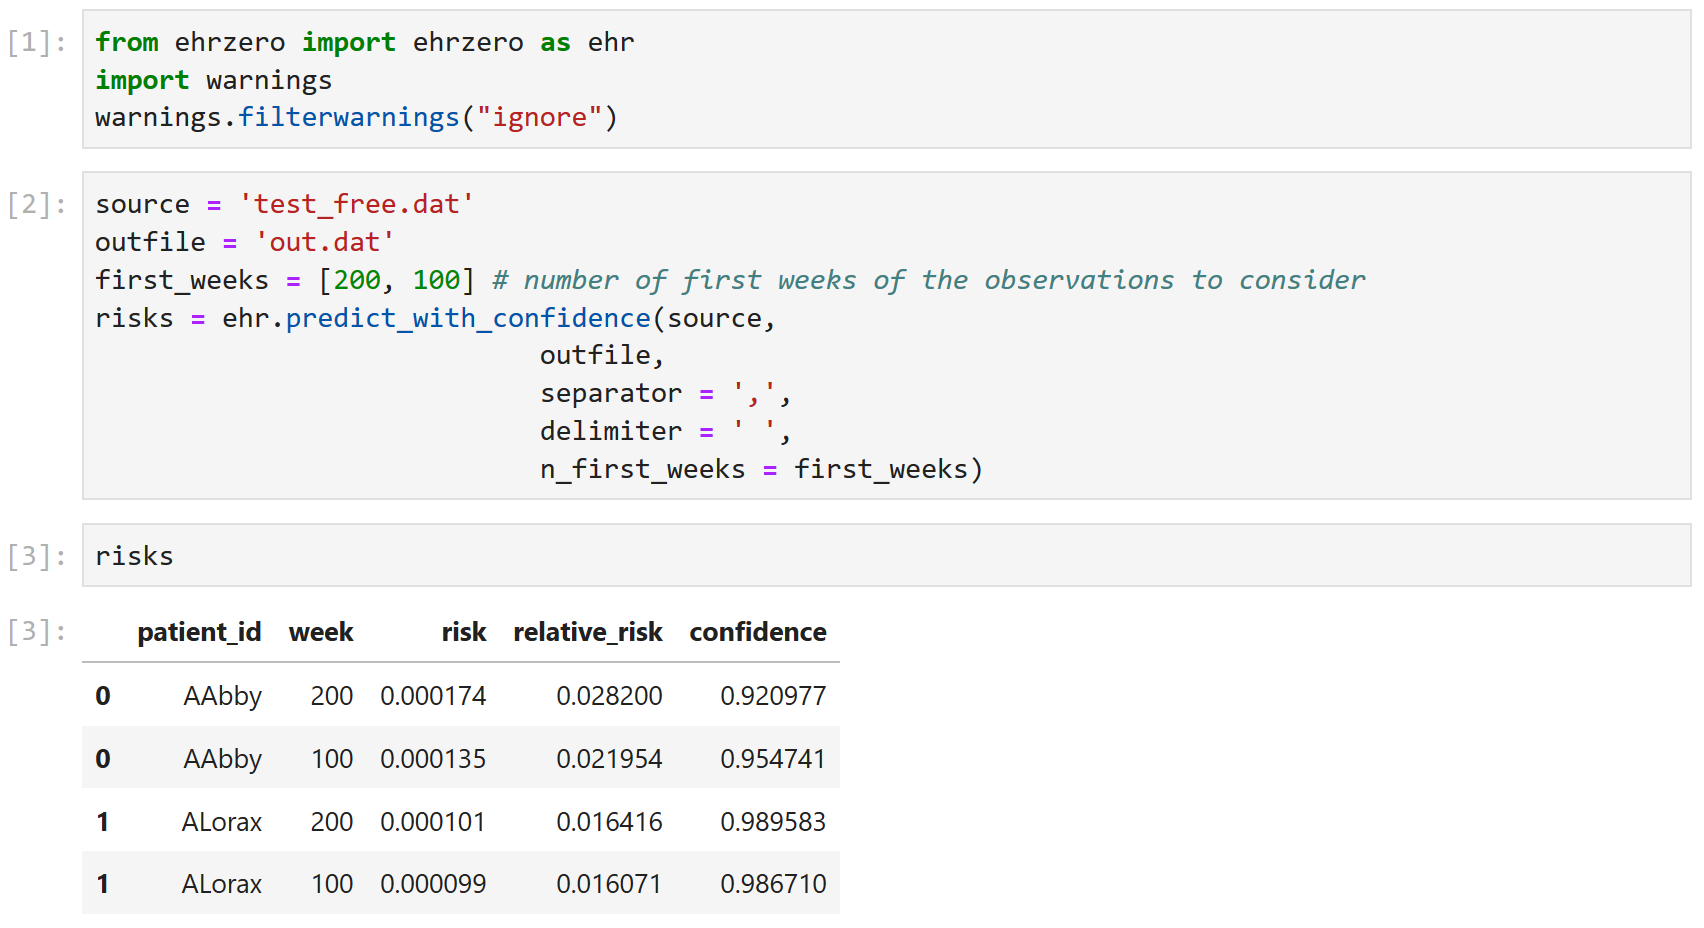
\includegraphics[width=.9\textwidth]{Figures/ehrzero_example}
\captionN{Python code prediction example}
\end{figure}

%###################################
\subsection{Prerequisites \& Installation}

The minimum prerequisites for running ehrzero are the following:
\begin{enumerate}
\item A x64 system running any flavor of Linux.
\item A working python 3.x installation
\item \texttt{scikit-learn}, version = \texttt{0.20.0}
\end{enumerate}

Installation:

\texttt{pip3 install ehrzero --user}

\subsection{EHR data format}

Diagnostic data stored in text file, one line per patient as follows: patient id, gender, and list of space-separated, comma-delineated diagnosis records, all separated by spaces. Each diagnosis record consists of the week since the start of the  observation, followed by a comma,  and the ICD-9 code of the diagnosis. 

Example of a patient line:

\texttt{Lorax,M 5,277.03 10,611.79 18,057.8 58,157.8 78,057.8 108,057.8 128,057.8 148,057.8}

\subsection{Sample Python code risk estimation}

Once the patient diagnostic data is in the required format, for function \texttt{predict\_with\_confidence} we specify the filepath of the data and the list of the cutoffs for the first weeks since the start of observations for the data we want to analyze. We also specify the separator and delimiter for the patients within file (space and comma are default values, but can be changed for user convenience).

The \texttt{predict\_with\_confidence} function returns the predicted risk of autism for every patient in the input file with all the specified numbers of first weeks to consider.

\subsection{Sample Python script risk estimation}

The script version is similar to the one mentioned before.

Once \texttt{ehrzero} package is installed, locate its directory and go to texttt{../ehrzero/example}. Select one of the \texttt{".dx"} or \texttt{".dat"} files in \texttt{/ehrzero/example/tests} as input and run the following command as an example:

\texttt{python zero.py -data tests/ZERO$\-$example.dat -outfile predictions.csv -n$\-$weeks 100 200 300 -Verbose 1}

\begin{figure}[!ht]
\centering
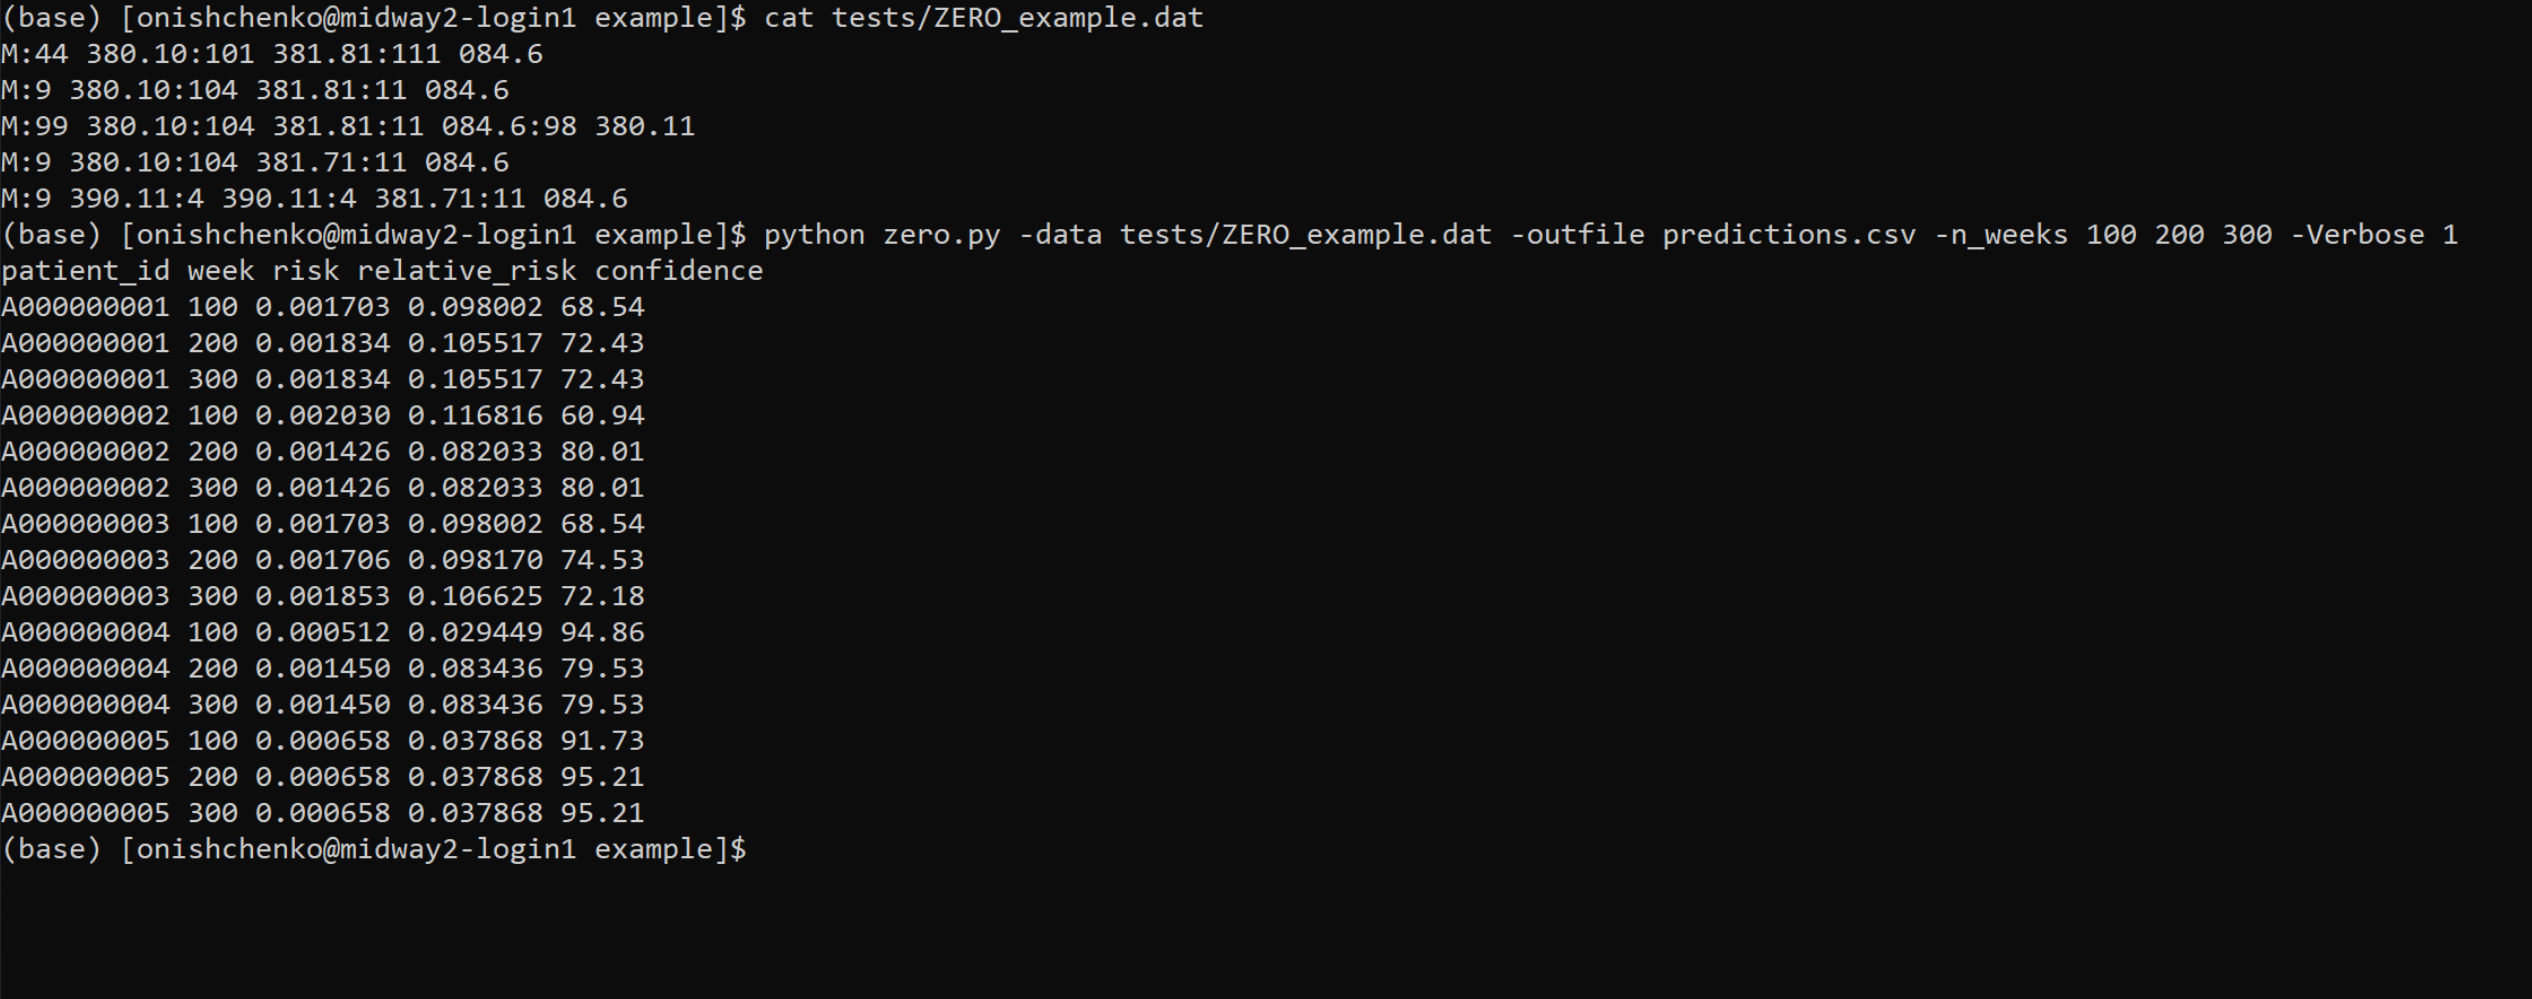
\includegraphics[width=.9\textwidth]{Figures/zero_py_example}
\captionN{Python script prediction example}
\end{figure}
% \clearpage

%\bibliographystyle{naturemag}
%\bibliography{mergedbib}




\end{document}

%  LocalWords:  comorbidities
